%\setcounter{chapter}{32}
\chapter{Generative Modeling Meets Representation Learning}\label{chapter:generative_modeling_and_representation_learning}

\section{Introduction}

This chapter is about models that unite the ideas of both generative modeling and representation learning. These models learn mappings both to and from data.%, and simultaneously satisfy the goals of both representation learning and generative modeling.

The intuition is that generative models map a simple base distribution (i.e., noise) to data, whereas representation learning maps data to simple underlying representations (\textbf{embeddings}). These two problems are, essentially, inverses of each other. Many algorithms explicitly treat them as inverse problems, where solving the problem in one direction can inform the solution in the other direction.

In \chap{\ref{chapter:neural_nets}}, we described neural nets as being a sequence of mappings from raw data to ever more abstracted representations, layer by layer. This perspective puts representation learning in the spotlight: deep learning is just representation learning! Let us now point out an alternative perspective: in backward order, deep nets are mappings from abstracted representations to ever more concrete representations of the data, layer by layer. This backward ordering is the direction in which deep generative networks work. This perspective puts the spotlight on generative modeling: deep learning is just generative modeling! Indeed both modeling directions are valid, and the full picture looks like this (\fig{\ref{fig:generative_modeling_and_representation_learning:rep_gen_schematic}}):
\begin{figure}[h!]
    \centerline{
    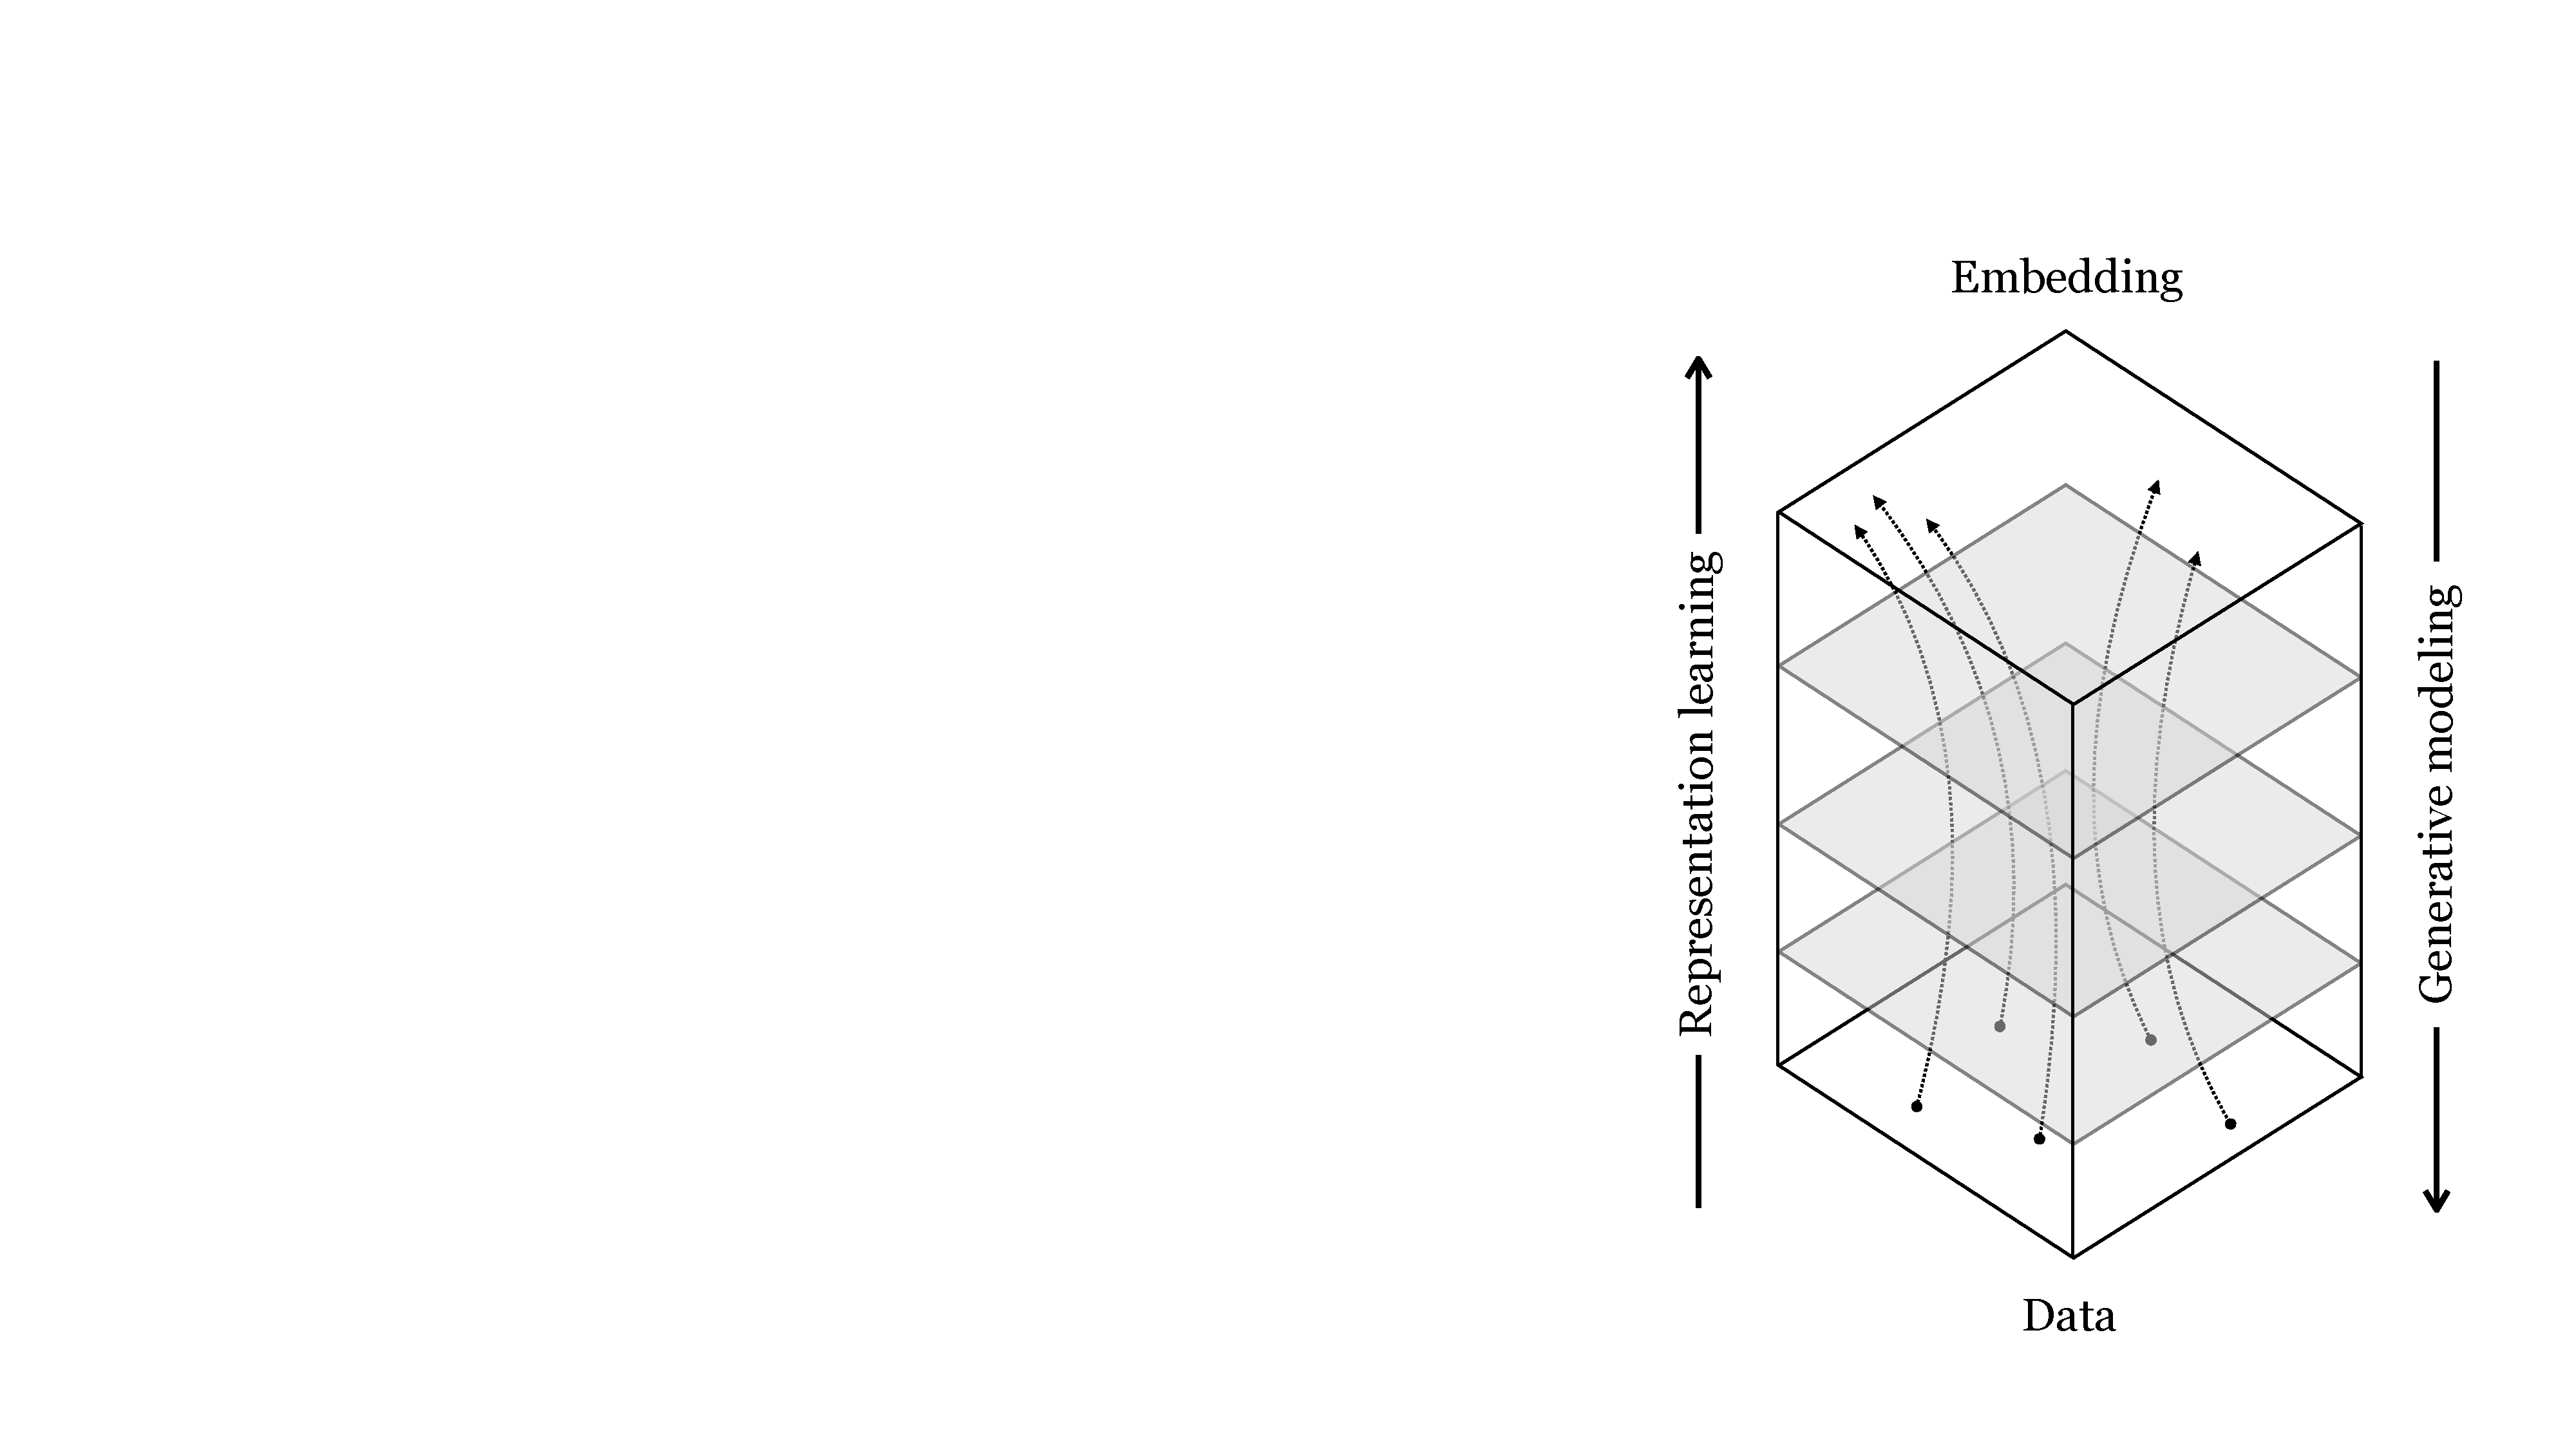
\includegraphics[width=0.35\linewidth]{./figures/generative_modeling_and_representation_learning/rep_gen_schematic.pdf}
    }
    \caption{The relationship between representation learning and generative modeling. Here we label one side as ``Data'' and the other as ``Embedding''; but what's the precise difference between these two things? Why is an RGB image data while a 100-dimensional vector of neural activations is an embedding? This is a question for you to think about; there is no correct answer.}
    \label{fig:generative_modeling_and_representation_learning:rep_gen_schematic}
\end{figure}
\marginnote{Moving backward through a net is also what backpropagation does, but it computes a different function: backpropagation computes the gradient $\nabla f$ whereas here we focus on the inverse $f^{-1}$.}[-3cm]


\section{Latent Variables as Representations}
\index{Latent variables}

In \chap{\ref{chapter:generative_models}}, we introduced generative models with latent variables $\mathbf{z}$. In that context, the role of the latent variable was to specify all unobserved factors that might affect the output of a model. For example, if the model predicts the color of a black and white photo, it is a mapping $g: \mathbf{x}, \mathbf{z} \rightarrow \mathbf{y}$, with $\mathbf{x}$ being the black and white input, $\mathbf{y}$ being the color output and $\mathbf{z}$ being any other information that needs to be known in order to make the mapping completely deterministic; for example, the color of a t-shirt which cannot be inferred solely from the black and white input. In the extreme case of unconditional generative models, all properties of the generated images are controlled by the latent variables.

What we did not mention in \chap{\ref{chapter:generative_models}}, but will focus on now, is that \textit{latent variables are representations of the data}. In the case of an unconditional generative model, the latent variables are a \textit{complete} representation of the data: all information in the data is represented in the latent variables.

Given this connection, this chapter will ask the following question: Are latent variables \textit{good} representations of the data? And can they be combined with other representation learning algorithms?

%The main idea is that latent variables are representations. 

%We have already seen representation learning as the problem of mapping data $\mathbf{x}$ to ``embedding" $\mathbf{z}$ and generative modeling as the problem of mapping ``noise" $\mathbf{z}$ to data $\mathbf{x}$. You may have wondered why we used the same variable name, $\mathbf{z}$, for these seemingly different things. The reason is because they are actually highly related! Both embeddings and noise are representations that have a deterministic functional relationship to the data, $\mathbf{z} = E(\mathbf{x})$ and $\mathbf{x} = G(\mathbf{z})$. An encoder $E$ performs the inverse functional role as a generator $G$.\marginnote{All generative models map a stochastic noise source to images, but not all interpret the noise source as latent random variables. For example, autoregressive models are fit without reference to any latent variables, and the noise source is only used during sampling.}[-2cm] The models we will describe in this chapter make the connection between noise and embeddings formally precise.

\section{Technical Setting}
We will consider random variables $\mathbf{z}$ and $\mathbf{x}$ related as follows, with $g$ being deterministic generator (i.e., decoder) and $f$ being a deterministic encoder:
\begin{align}
    &\mathbf{x} \sim p_{\texttt{data}} &\mathbf{z} \sim p_{\mathbf{z}} \\
    &\hat{\mathbf{z}} = f(\mathbf{x}) &\hat{\mathbf{x}} = g(\mathbf{z})
\end{align}
where $f$ and $g$ will be trained so that $g \approx f^{-1}$, which means that $\hat{\mathbf{x}} \approx \mathbf{x}$ and $\hat{\mathbf{z}} \approx \mathbf{z}$. In \fig{\ref{fig:representation_learning:rep_learning_schematic}}, we sketched how representation learning maps from a data domain to a simple embedding space. We can now put that diagram side by side with the equivalent diagram for generative modeling. Notice again how they are just the same thing in opposite directions (\fig{\ref{fig:generative_modeling_and_representation_learning:genrep_schematic}}):
\begin{figure}[h!]
    \centerline{
    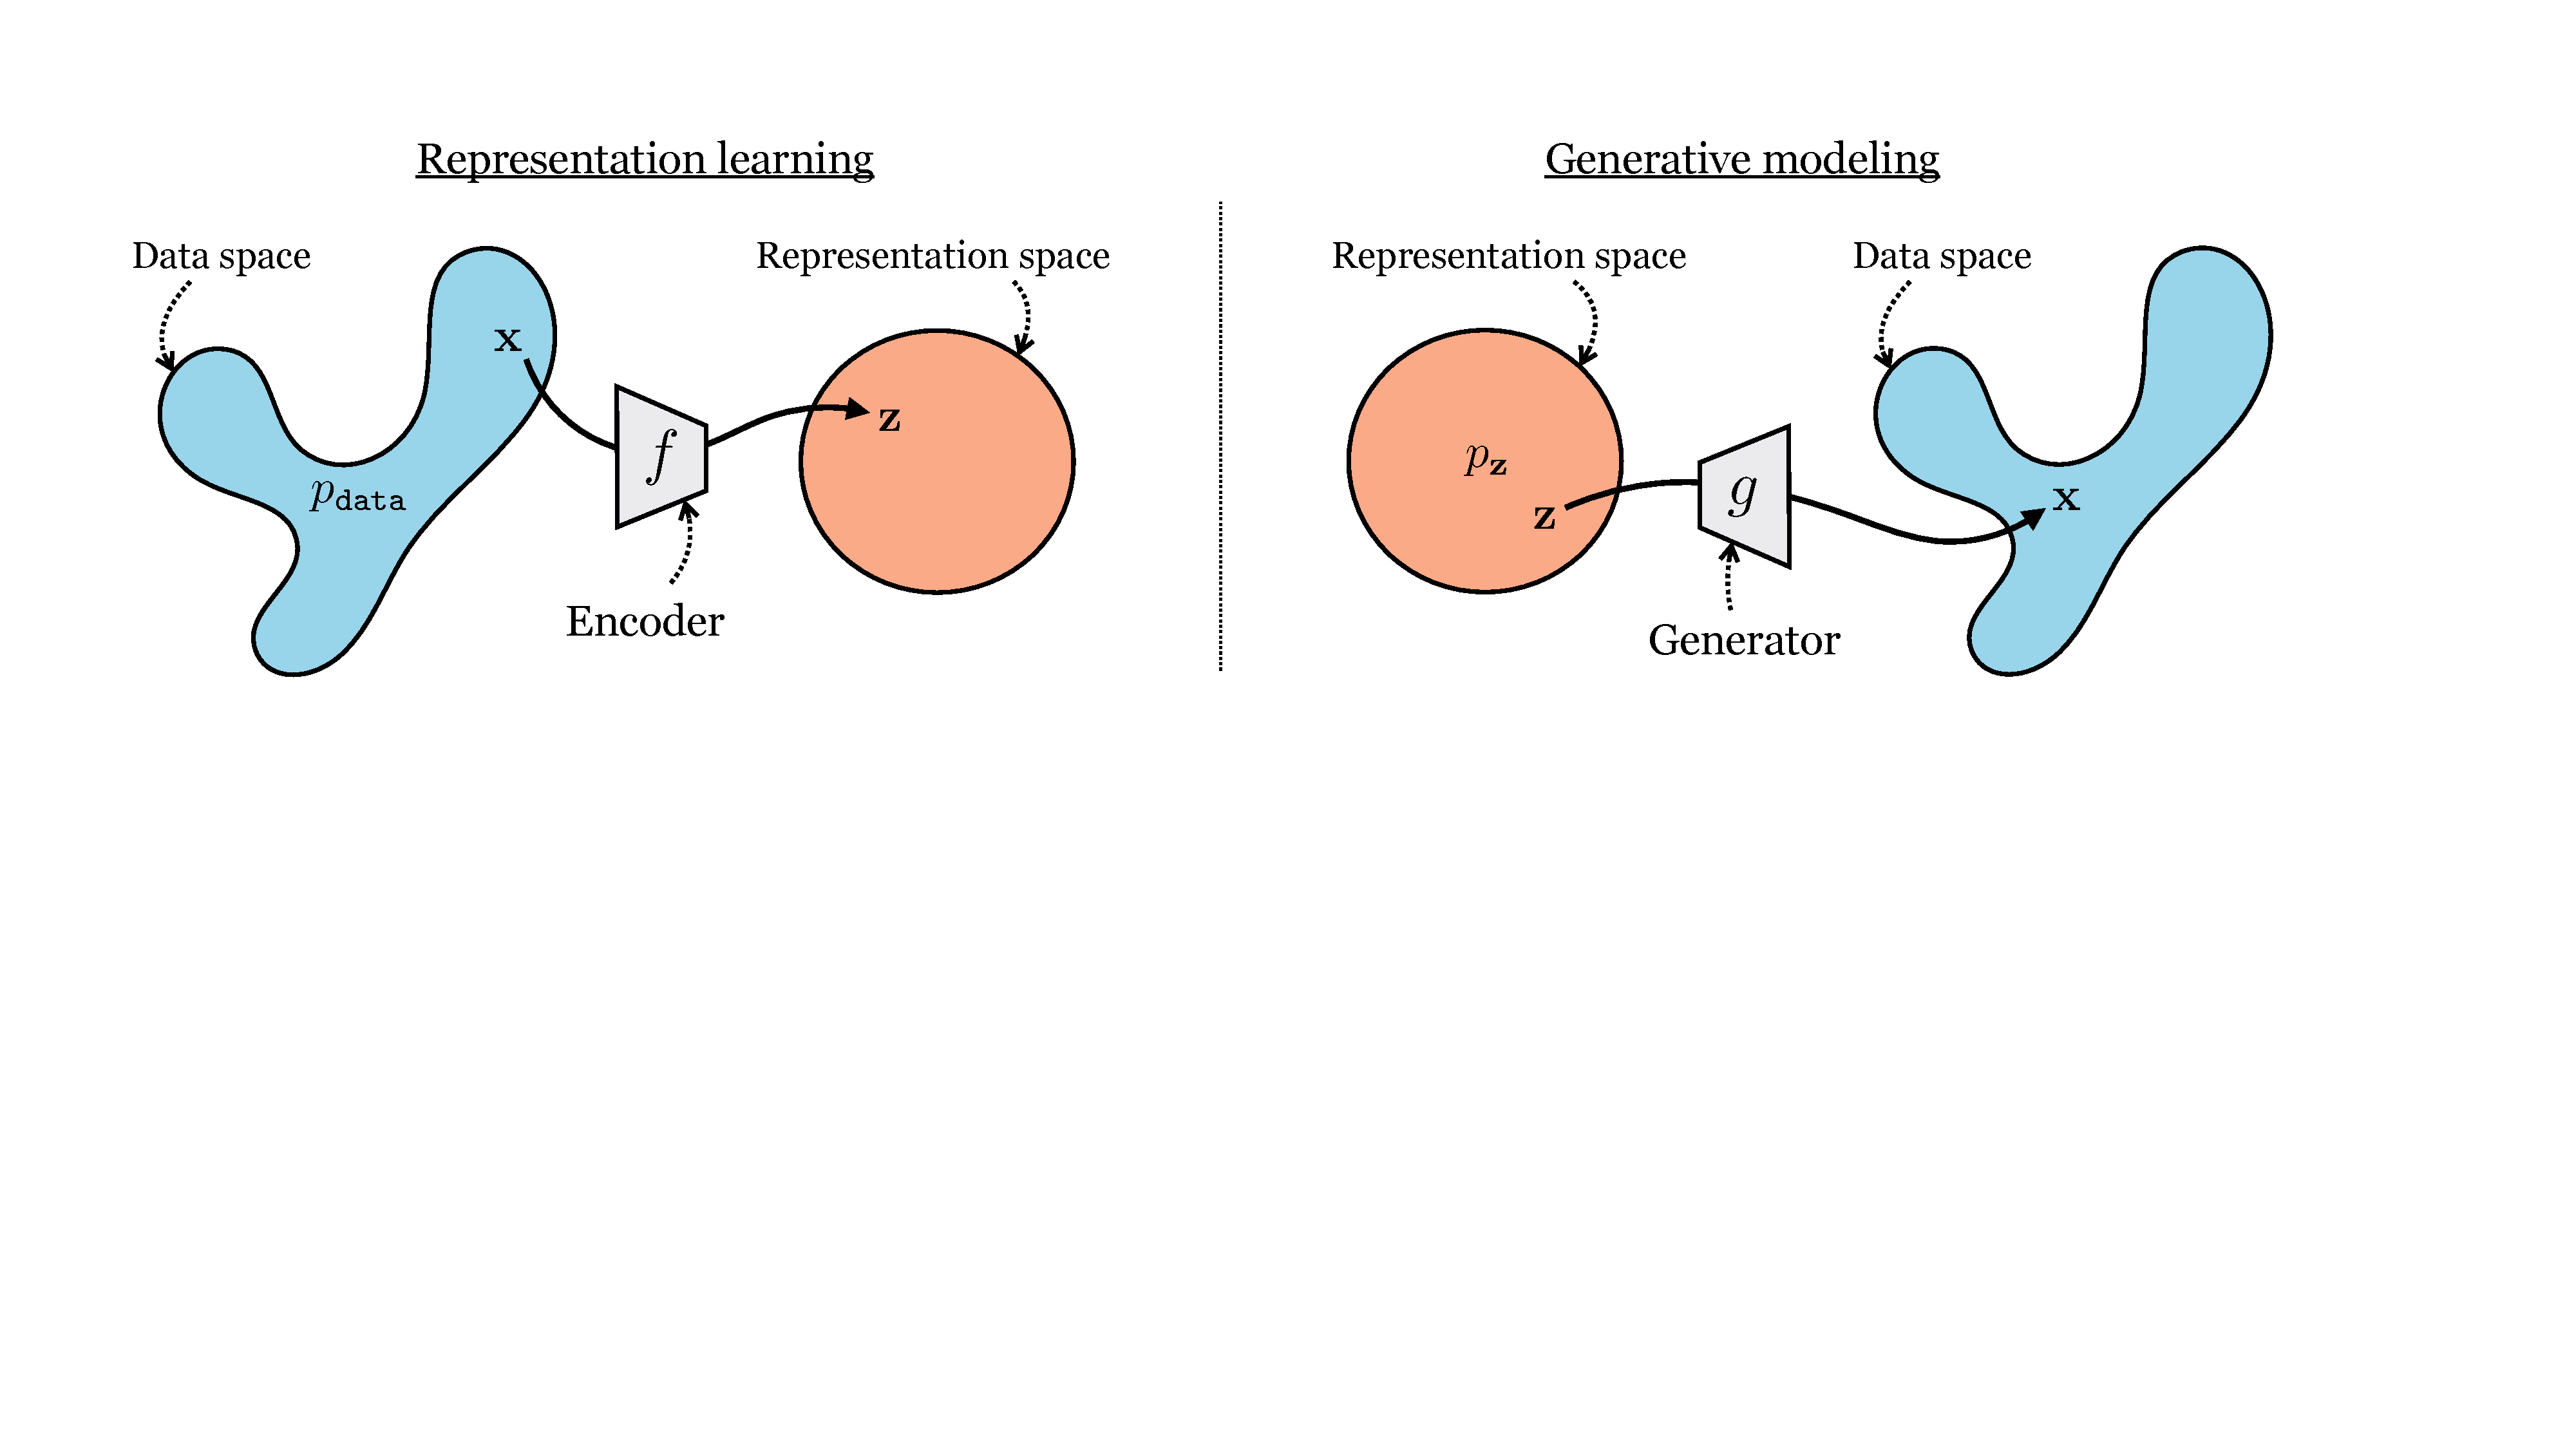
\includegraphics[width=1.0\linewidth]{./figures/generative_modeling_and_representation_learning/genrep_schematic.pdf}
    }
    \caption{Generative modeling performs the opposite mapping from representation learning.}
    \label{fig:generative_modeling_and_representation_learning:genrep_schematic}
\end{figure}

The critical thing in most generative models, which is not necessarily true for representation learning models, is that we assume we know the distribution $p_{\mathbf{z}}$, and typically it has a simple form such as a unit Gaussian. Knowing this distribution allows us to sample from it and then generate images via $g$.

One of the most important quantities we will measure is the data log likelihood function $L(\{\mathbf{x}\}_{i=1}^N, \theta)$, which measures the log likelihood of the data under the model $p_{\theta}$:
\begin{align}
    L(\{\mathbf{x}^{(i)}\}_{i=1}^N, \theta) = \sum_{i=1}^N \log p_{\theta}(\mathbf{x}^{(i)})
\end{align}
Many methods use a max likelihood objective, optimizing $L$ with respect to $\theta$. To compute the likelihood function, we need to compute $p_{\theta}(\mathbf{x})$. One way to express this function is as the \index{Marginal likelihood}\textbf{marginal likelihood} of $\mathbf{x}$, marginalizing over all unobserved latent variables $\mathbf{z}$:
\begin{align}
    p_{\theta}(\mathbf{x}) = \int_{\mathbf{z}} p_{\theta}(\mathbf{x} \given \mathbf{z})p_{\mathbf{z}}(\mathbf{z})d\mathbf{z}\label{eqn:generative_modeling_and_representation_learning:marginal_likelihood_p}
\end{align}
%Here $\mathbf{z}$ are the latent variables. Given an observation $\mathbf{x}$, we may integrate over the latent variables to calculate its probability. 
The advantage of expressing $p_{\theta}(\mathbf{x})$ in this way is that, assuming we know $p_{\mathbf{z}}$, the rest of the modeling problem is reduced to learning the conditional distribution $p_{\theta}(X \given \mathbf{z})$, which itself can be straightforwardly modeled using $g$. For example, we could model $p_{\theta}(X \given \mathbf{z}) = \mathcal{N}(\mu = g(\mathbf{z}), \sigma = \mathbf{1})$, that is, just place a unit Gaussian distribution over $X$ centered on $g(\mathbf{z})$.

%We can also write the marginal likelihood for the probability of a latent vector $\mathbf{z}$ expressed as an integral over $p_{\texttt{data}}$, given a model of the conditional distribution of $\mathbf{z}$ given $\mathbf{x}$:
%\begin{align}
%    q_{\psi}(\mathbf{x}) = \int_{\mathbf{x}} q_{\psi}(\mathbf{z} | \mathbf{x})p_{\texttt{data}}(\mathbf{x})d\mathbf{x}\label{eqn:generative_modeling_and_representation_learning:marginal_likelihood_q}
%\end{align}
%Following standard notation, we use $p$ to refer to probability distributions over data and $q$ to refer to probability distributions over latents.

The integral in \eqn{\ref{eqn:generative_modeling_and_representation_learning:marginal_likelihood_p}} %and \ref{eqn:generative_modeling_and_representation_learning:marginal_likelihood_q} are 
is expensive so most generative models either sidestep the need to explicitly calculate it, or approximate it. We will examine one such strategy next.

\section{Variational Autoencoders}\label{sec:generative_modeling_and_representation_learning:VAEs}
\index{Variational autoencoder}

In the next sections we will examine the \textbf{variational autoencoder} (\textbf{VAE})~\cite{kingma2013auto,kingma2019introduction}, which is a model that turns an autoencoder into a generative model that can synthesize data.

\subsection{The Decoder of an Autoencoder is a Data Generator}
In \chap{\ref{chapter:representation_learning}} we learned about autoencoders. These are models that learn an embedding that can be decoded to reconstruct the input data. You may already have noticed that the decoder of an autoencoder looks just like a generator. It is a mapping from a representation of the data, $\mathbf{z}$, back to the data itself, $\mathbf{x}$. Given a $\mathbf{z}$, we can synthesize an image by passing it through the decoder of the autoencoder (\fig{\ref{fig:generative_modeling_and_representation_learning:autoencoder_to_generative_model}}):
\begin{figure}[h!]
    \centerline{
    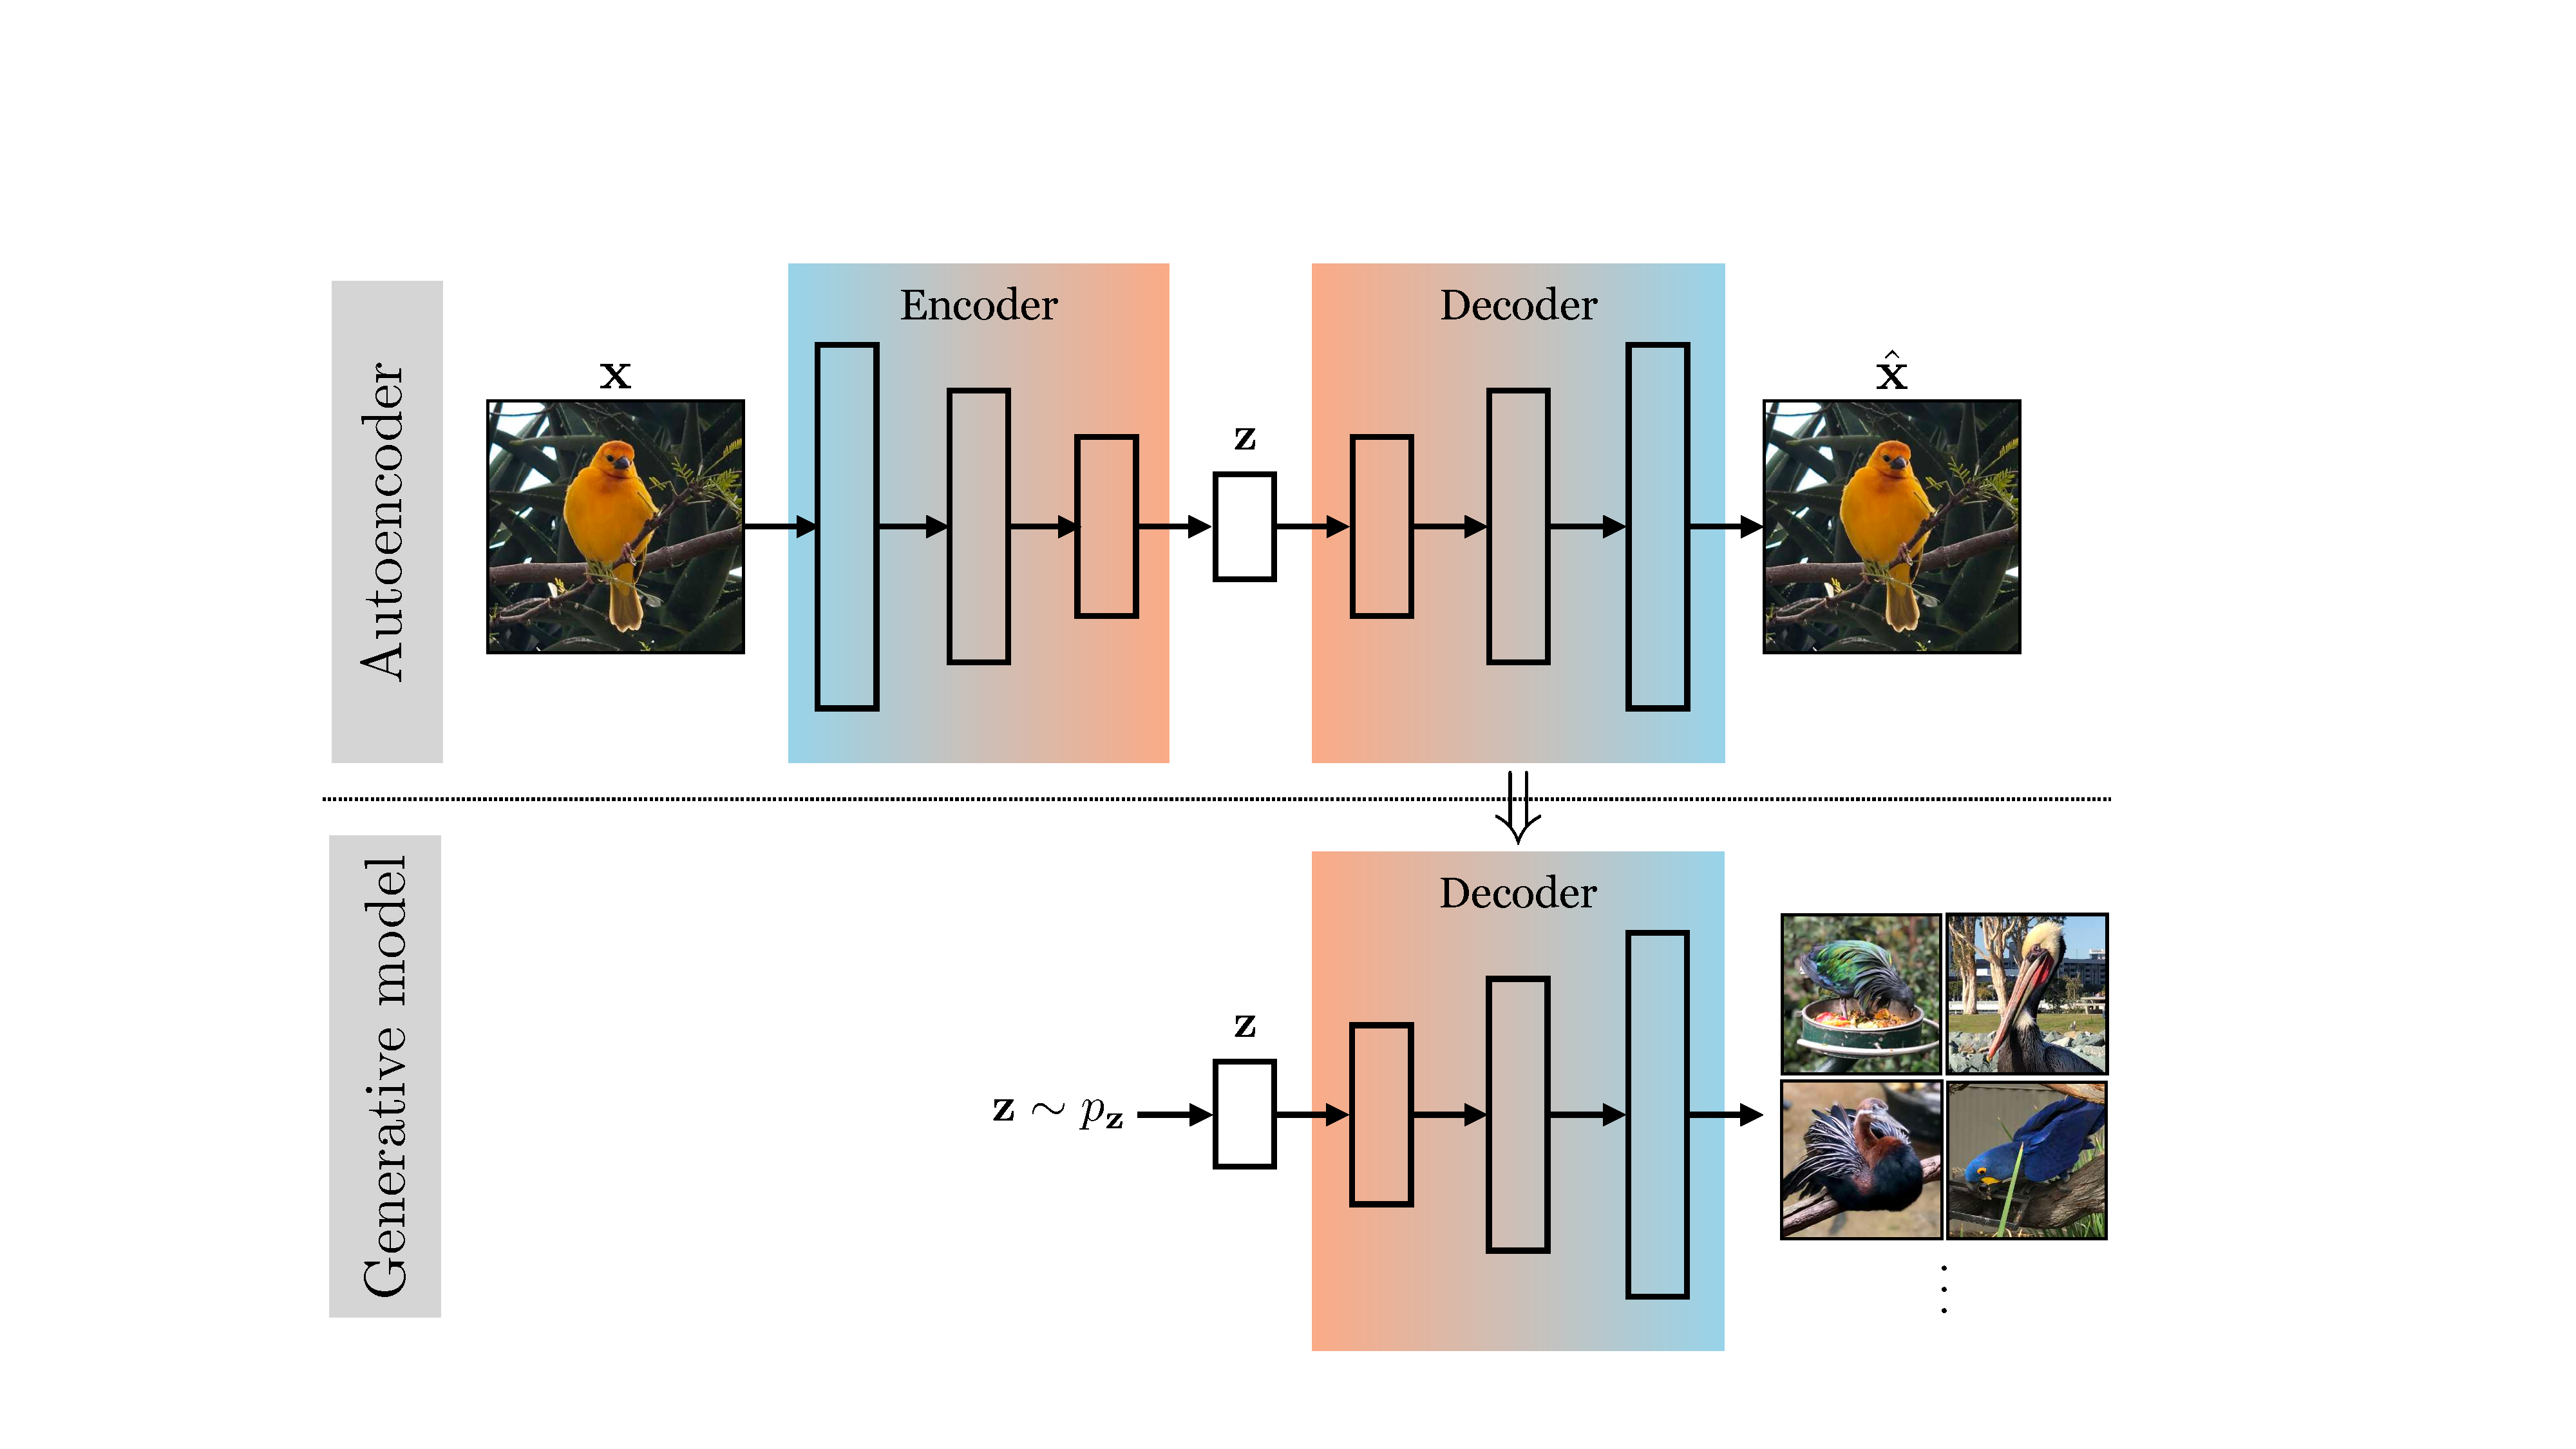
\includegraphics[width=0.8\linewidth]{./figures/generative_modeling_and_representation_learning/autoencoder_to_generative_model.pdf}
    }
    \caption{The relationship between an autoencoder and a generative model.}
    \label{fig:generative_modeling_and_representation_learning:autoencoder_to_generative_model}
\end{figure}

But how do we get this $\mathbf{z}$? One goal of generative modeling is to be able to make up random images from scratch. So we need a distribution from which we can sample different $\mathbf{z}$ from scratch, that is, we need $p_{\mathbf{z}}$. An autoencoder doesn't directly give us this. You might ask, what if, after training an autoencoder, you just sample a random $\mathbf{z}$, say from a unit Gaussian, and feed it through the decoder? The problem is that this sample might be very different from what the decoder was trained on, and it therefore might not map to a natural looking image. For example, maybe the encoder has learned to map all images to embeddings far from the origin; then a unit Gaussian $\mathbf{z}$ would be far out of distribution and the decoder's behavior could be arbitrary for this out-of-distribution input. %Sure we can get $\mathbf{z}$'s by encoding images as $F(\mathbf{x})$, but then we need a way to sample random images from scratch, and we are back where we started.

In general, the embedding space of an autoencoder might be just as complicated to model as the data space we started with, as indicated in \fig{\ref{fig:generative_modeling_and_representation_learning:autoencoder_complicated_latent_space}}:%\marginnote{Due to various implicit biases, autoencoder embeddings may turn out to be simpler than the data they are trained on.}
\begin{figure}[h!]
    \centerline{
    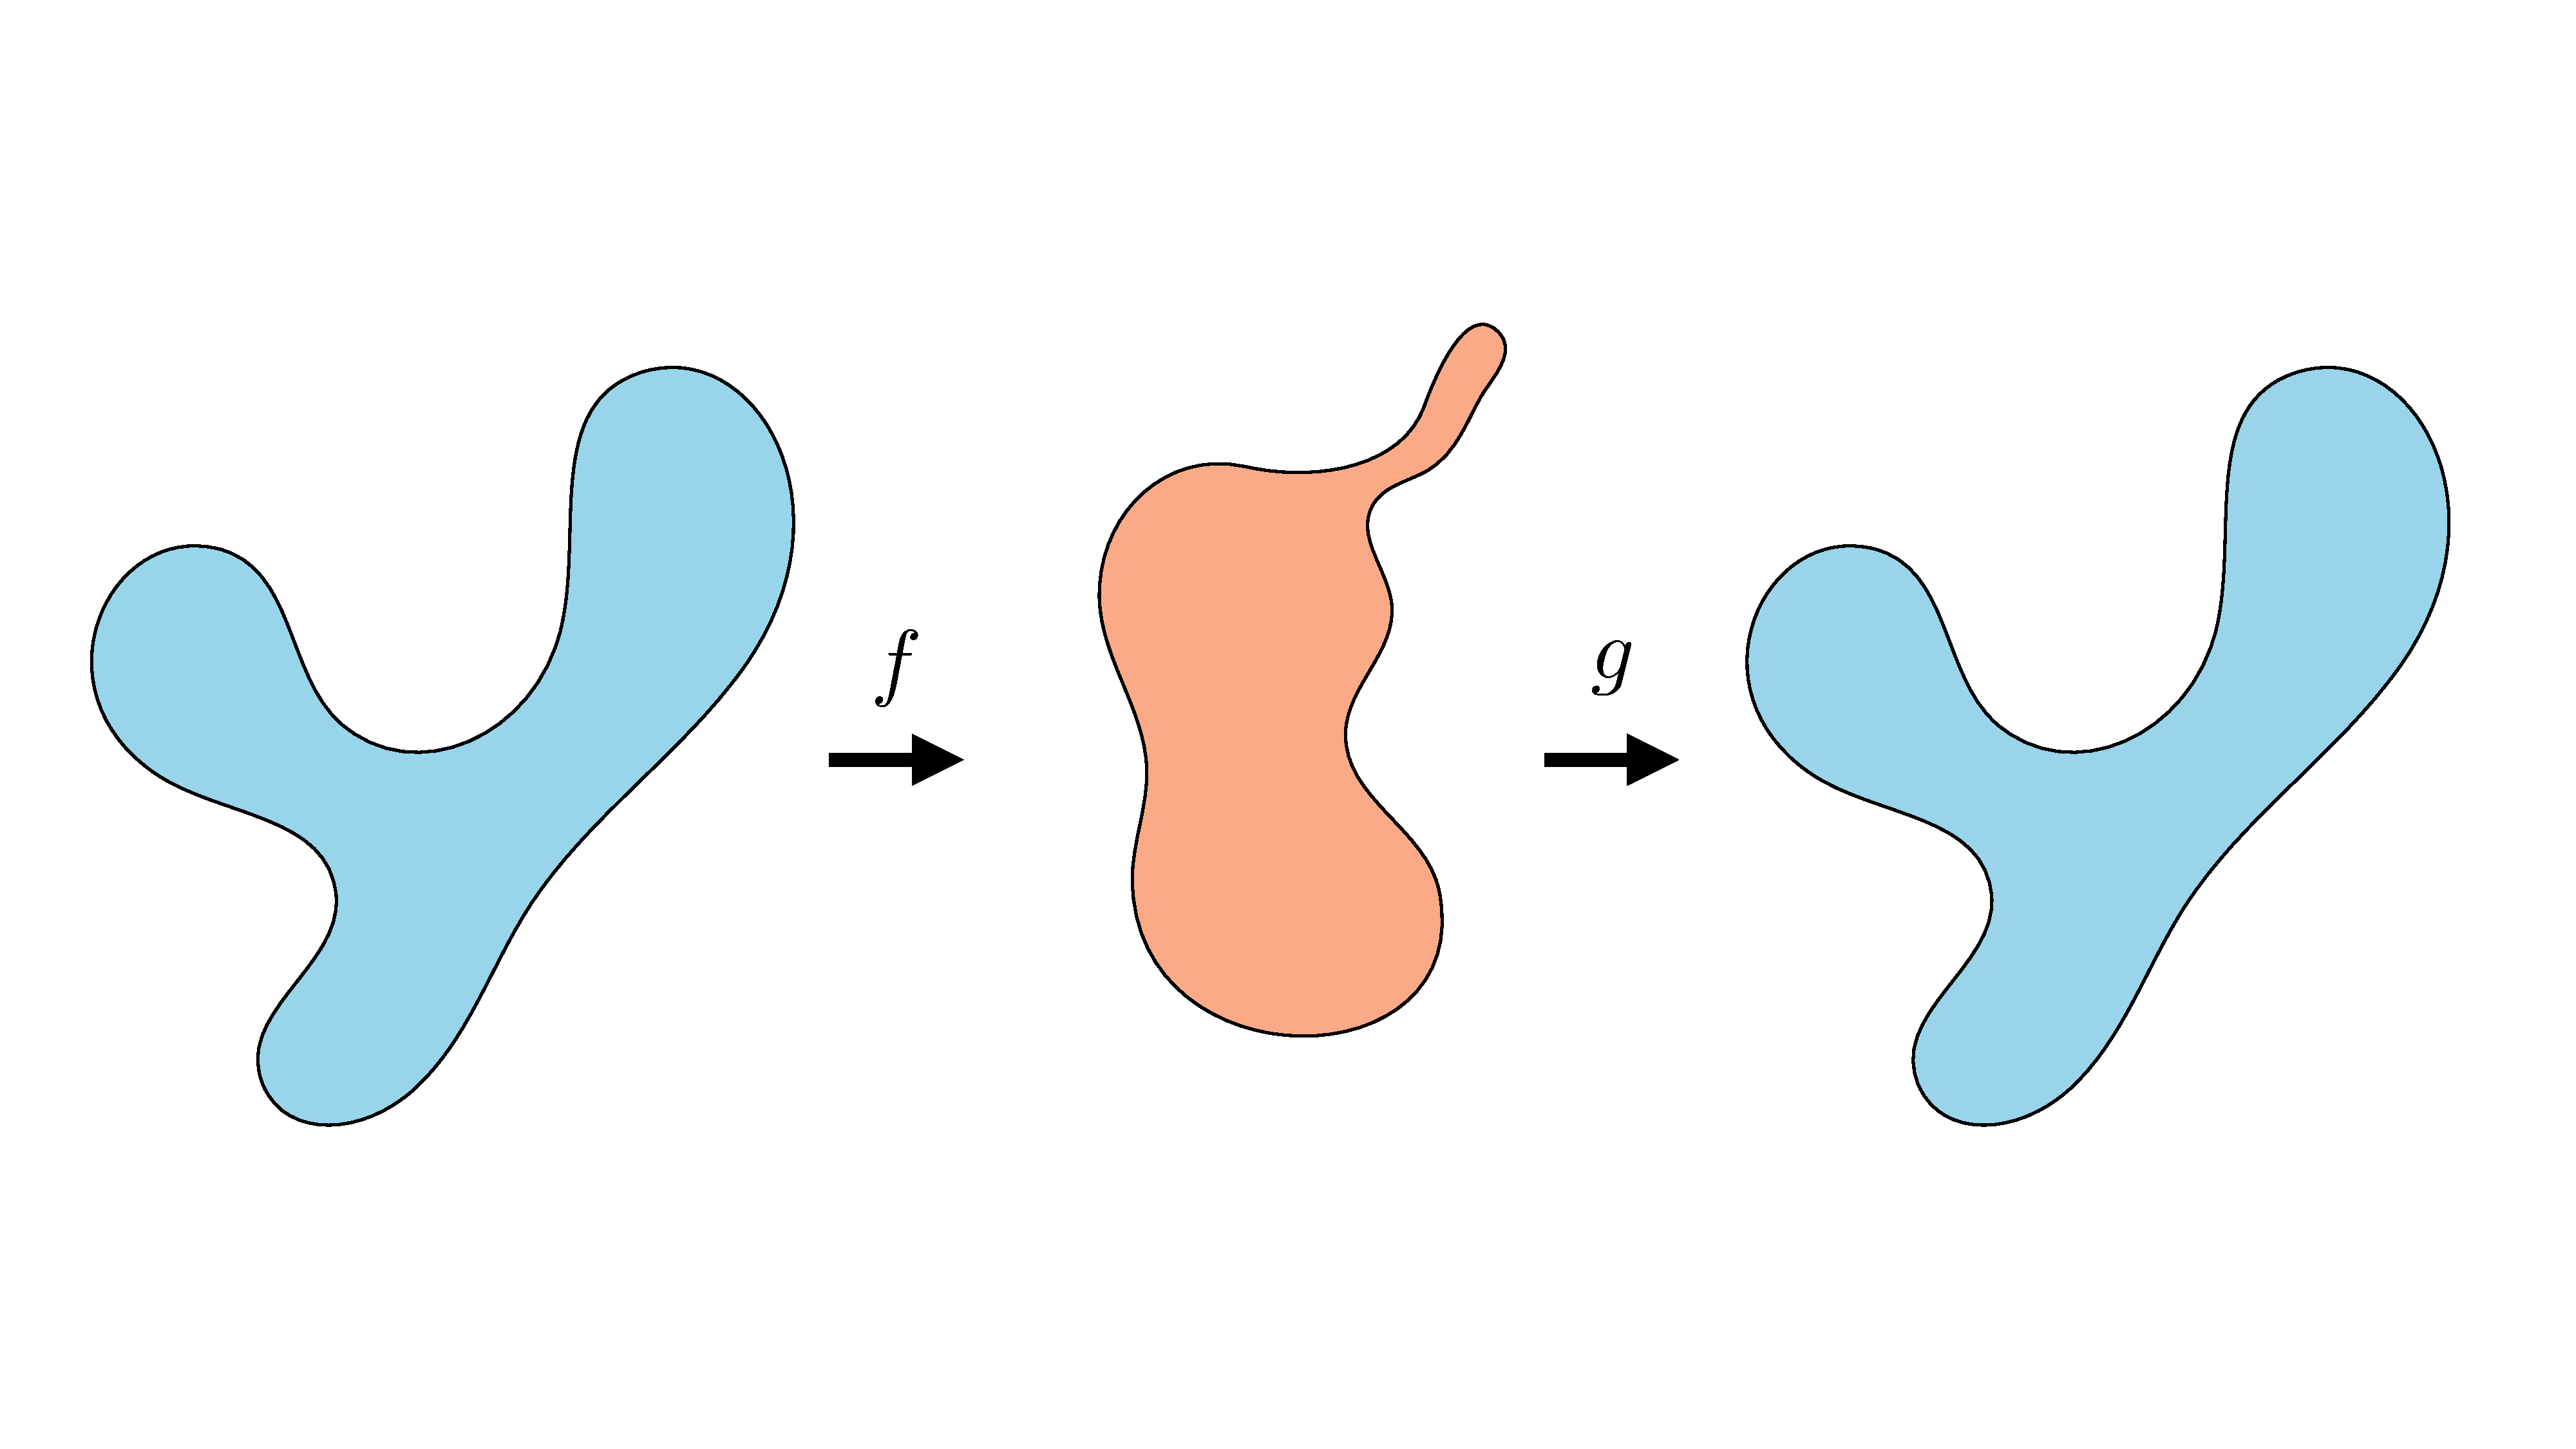
\includegraphics[width=0.6\linewidth]{./figures/generative_modeling_and_representation_learning/autoencoder_complicated_latent_space.pdf}
    }
    \caption{The latent space of an autoencoder can be just as complex as the data space.}
    \label{fig:generative_modeling_and_representation_learning:autoencoder_complicated_latent_space}
\end{figure}


VAEs are a way to turn an autoencoder into a proper generative model, which can be sampled from and which maximizes data likelihood under a formal probabilistic model. The trick is very simple: just take a vanilla autoencoder and (1) regularize the latent distribution to squish it into a Gaussian (or some other base distribution), (2) add noise to the output of the encoder. In code, it can be as simple as a two line change!

Okay, but seeing \textit{why} this is the right and proper thing to do requires quite a bit of math. We will derive it now, using a different approach than in most texts. We think this approach makes it easier to intuit what is going on. See \cite{kingma2019introduction} for the more standard derivation.

\subsection{The VAE Hypothesis Space}

VAEs are max likelihood generative models, which maximize the likelihood function $L$ in \eqn{\ref{eqn:generative_modeling_and_representation_learning:marginal_likelihood_p}}. What distinguishes them from other max likelihood models is their particular hypothesis space and optimization algorithm. We will first describe the hypothesis space.

Remember the Gaussian generative model from \chap{\ref{chapter:generative_models}} (i.e., fitting a Gaussian to data)? We stated that this model is too simple for most purposes, but can form the basis for more flexible density models, which work by combining a lot of simple distributions. We gave one example in \chap{\ref{chapter:generative_models}}: autoregressive models, which model a complicated distribution as a product over many simple conditional distributions. VAEs follow a slightly different strategy: they model complicated distributions as \textit{sums} of simple distributions.

In particular, VAEs are \index{Mixture model}\textbf{mixture models}, and the most common kind of VAE is a \index{Gaussian mixture model}\textbf{mixture of Gaussians}.\marginnote{Mixture models are probability models of the form $P(\mathbf{x}) = \sum_i w_ip_i(\mathbf{x})$.}[-1cm] The mixture of Gaussians model is in fact classical model that represents a density as a weighted sum of Gaussian distributions:
\begin{align}
    p_{\theta}(\mathbf{x}) = \sum_{i=1}^k w_i \mathcal{N}(\mathbf{x}; \mathbf{\mu}_i, \mathbf{\Sigma}_i) \quad\quad \triangleleft \quad\text{mixture of Gaussians}
\end{align}
where the parameters are $\theta = \{\mathbf{\mu}_i, \mathbf{\Sigma}_i\}_{i=1}^k$, that is, the mean and variance of all Gaussians in the mixture. Unlike classical Gaussian mixture models, VAEs use an \textit{infinite} mixture of Gaussians, that is, $k \rightarrow \infty$.

But wait, how can we parameterize an infinite mixture? We can't learn an infinite set of means and variances. The trick we will use is to make the mean and variance be \textit{functions} of an underlying continuous variable.\marginnote{You can think of a function as the \textit{infinite set} of values a variable takes on over some domain.} The function the VAE uses is $g_{\theta}$. For notational convenience, we decompose this function into $g_{\theta}^{\mu}$ and $g_{\theta}^{\Sigma}$ to separately model the means and variances of the Gaussians in the infinite mixture. Next we need a continuous domain to integrate our mixture over, and as a simple choice, we will use the unit Gaussian distribution. Then our infinite mixture can be described as:
%\textit{parameterize the parameters}: the infinite set of \textit{parameters} can be described by a finite set of \textit{hyperparameters}. A VAE does this with a neural net $g_{\theta}$ that 
%we will use is to introduce \textit{continuous} latent variables to model the infinite mixture. Then we can marginalize over these latents to obtain the marginal likelihood just like in Eqn. \ref{eqn:generative_modeling_and_representation_learning:marginal_likelihood_p}. 
%Following this strategy, the standard hypothesis for VAEs is:
% \begin{align}
%     &p_{\theta}(\mathbf{x}) = \int_{\mathbf{z}} p_{\theta}(\mathbf{x}|\mathbf{z})p_{\mathbf{z}}(\mathbf{z})d\mathbf{z}\\
%     &\quad\quad p_{\theta}(\mathbf{x}|\mathbf{z}) = \mathcal{N}(\mathbf{x}; g^{\mu}_{\theta}(\mathbf{x}), g^{\Sigma}_{\theta}(\mathbf{x}))\\
%     &\quad\quad p_{\mathbf{z}}(\mathbf{z}) = \mathcal{N}(\mathbf{z}; \mathbf{0}, \mathbf{1})
% \end{align}
\begin{align}
    p_{\theta}(\mathbf{x}) = \int_{\mathbf{z}} \underbrace{\mathcal{N}(\mathbf{x}; g^{\mu}_{\theta}(\mathbf{z}), g^{\Sigma}_{\theta}(\mathbf{z}))}_{p_{\theta}(\mathbf{x} \shortgiven \mathbf{z})}\underbrace{\mathcal{N}(\mathbf{z}; \mathbf{0}, \mathbf{I})}_{p_{\mathbf{z}}(\mathbf{z})}d\mathbf{z} \quad\quad \triangleleft \quad\text{VAE hypothesis space}
\end{align}
Notice that this equation—an infinite mixture of Gaussians parameterized by a function $g_{\theta}$—has exactly the same form as the marginal likelihood in \eqn{\ref{eqn:generative_modeling_and_representation_learning:marginal_likelihood_p}}. What we have done is model an infinite mixture as an integral that marginalizes over a continuous latent variable.

You can think about this as transforming a base distribution $p_{\mathbf{z}}$ to a modeled distribution $p_{\theta}$ by applying a deterministic mapping $g_{\theta}$ and then putting a blip of Gaussian probability around each point in the range of this mapping. If you sample a few of the Gaussians in this infinite mixture, they might look like this (\fig{\ref{fig:generative_modeling_and_representation_learning:gmm_vs_vae}}):
\begin{figure}[h!]
    \centerline{
    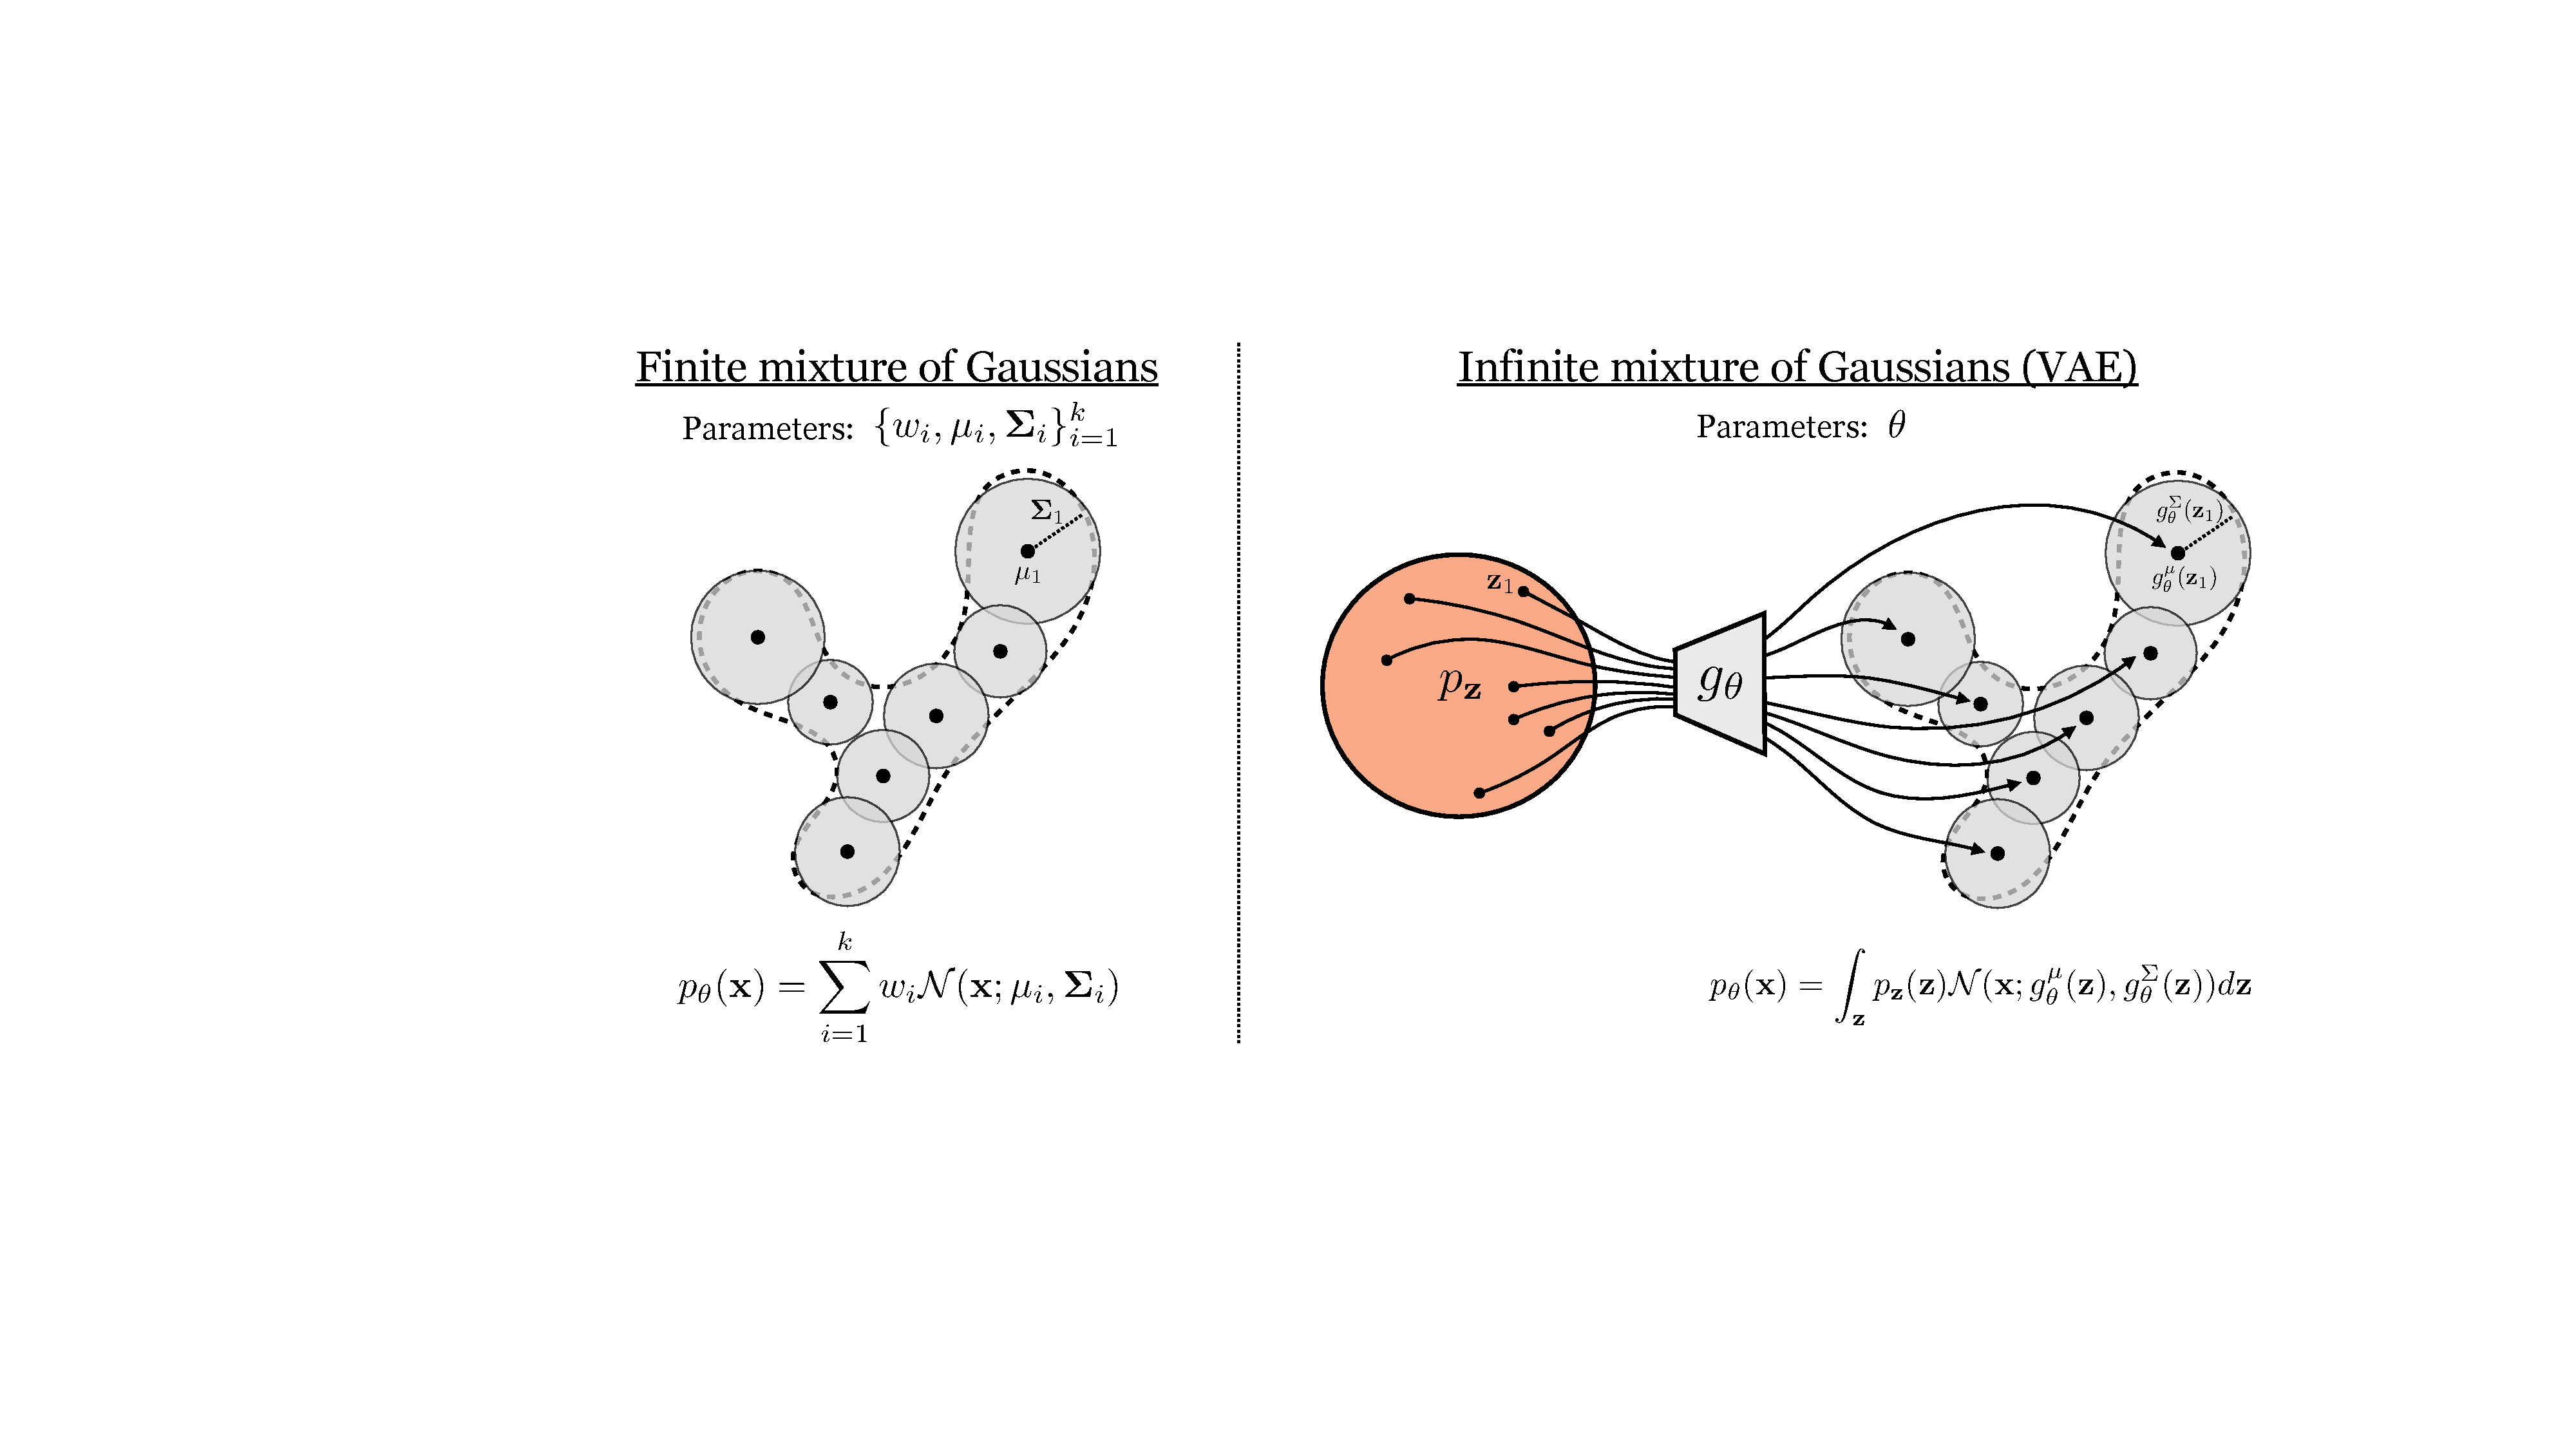
\includegraphics[width=0.9\linewidth]{./figures/generative_modeling_and_representation_learning/gmm_vs_vae.pdf}
    }
    \caption{From a finite mixture of Gaussians to an infinite mixture.}
    \label{fig:generative_modeling_and_representation_learning:gmm_vs_vae}
\end{figure}

While we have chosen Gaussians for $p_{\theta}(\mathbf{x} \given \mathbf{z})$ and $p_{\mathbf{z}}(\mathbf{z})$ in this example, VAEs can also be constructed using other base distributions, even complicated ones. For example, we could make an infinite mixture of the autoregressive distributions we saw in \chap{\ref{chapter:generative_models}}. In this sense, mixture models are metamodels, and their components can themselves be any of the density models we have learned about in this book, including other mixture models.


\subsection{Optimizing VAEs}
\marginnote{Wait, a whole section on optimization? Didn't this book say that general-purpose optimizers (like backpropagation) are often sufficient in the deep learning era? Yes. \textit{But only if you can actually compute the objective and its gradient}. The issue here is that the VAE's objective is \textit{intractable}. Its exact computation requires integrating over an infinite set of deep net forward passes. The difficulty of optimizing VAEs lies in the difficulty of approximating this intractable objective. Once we derive our approximation, optimization again will be easy: just apply backpropagation on this approximate loss.}[-1.2cm]
With the objective and hypothesis given previously, we can now fully define the VAE learning problem:
\begin{align}
    \theta^* &= \argmax_{\theta} L(\{\mathbf{x}^{(i)}\}_{i=1}^N, \theta)\\
    &= \argmax_{\theta} \sum_{i=1}^N \log \underbrace{\int_{\mathbf{z}} \overbrace{\mathcal{N}(\mathbf{x}^{(i)}; g^{\mu}_{\theta}(\mathbf{z}), g^{\Sigma}_{\theta}(\mathbf{z}))}^{p_{\theta}(\mathbf{x}^{(i)} \shortgiven \mathbf{z})} \overbrace{\mathcal{N}(\mathbf{z}; \mathbf{0}, \mathbf{I})}^{p_{\mathbf{z}}(\mathbf{z})}d\mathbf{z}}_{p_{\theta}(\mathbf{x}^{(i)})}\label{eqn:generative_modeling_and_representation_learning:vae_learning_problem1}
\end{align}

\subsubsection{Trick 1: Approximating the objective via sampling} 
The integral for $p_{\theta}(\mathbf{x}^{(i)})$ does not necessarily have a closed form since $g_{\theta}$ may be an arbitrarily complex function. Therefore, we need to approximate this integral numerically. The first trick we will use is a \textit{Monte Carlo estimate} of this integral:
\begin{align}
    p_{\theta}(\mathbf{x}) &= \int_{\mathbf{z}} p_{\theta}(\mathbf{x} \given \mathbf{z})p_{\mathbf{z}}(\mathbf{z})d\mathbf{z} \label{eqn:generative_models_and_representation_learning:vae_likelihood}\\
    &= \mathbb{E}_{\mathbf{z}\sim p_{\mathbf{z}}(\mathbf{z})}[p_{\theta}(\mathbf{x} \given \mathbf{z})]\\
    &\approx \frac{1}{M} \sum_{j=1}^M p_{\theta}(\mathbf{x} \given \mathbf{z}^{(j)}), \quad \mathbf{z}^{(j)} \sim p_{\mathbf{z}} \label{eqn:generative_models_and_representation_learning:vae_likelihood_monte_carlo_estimate}
\end{align}
We could stop here, as the learning problem is now written in a closed differentiable form:
\begin{align}
    \theta^* &= \argmax_{\theta} \frac{1}{M} \sum_{i=1}^N \log \sum_{j=1}^M \overbrace{\mathcal{N}(\mathbf{x}^{(i)}; g^{\mu}_{\theta}(\mathbf{z}^{(j)}), g^{\Sigma}_{\theta}(\mathbf{z}^{(j)}))}^{p_{\theta}(\mathbf{x}^{(i)} \shortgiven \mathbf{z}^{(j)})}\label{eqn:generative_modeling_and_representation_learning:vae_learning_problem1}
\end{align}
As long as $g_{\theta}$ is a differentiable neural net, we can proceed with optimization via backpropagation. In practice, on each iteration of backpropagation, we would collect a batch of random samples $\{\mathbf{x}^{(i)}\}_{i=1}^{B_1} \sim p_{\texttt{data}}$ from the training set and a batch of random latents $\{\mathbf{z}^{(j)}\}_{j=1}^{B_2} \sim p_{\mathbf{z}}$ from the unit Gaussian distribution (with $B_1$ and $B_2$ being batch sizes). Then we would pass each of the $\mathbf{z}$ samples through our net $g_{\theta}$, which yields a Gaussian under which we can evaluate each $\mathbf{x}$ sample. After evaluating and summing up the log probabilities, we would run a backward pass to update the parameters $\theta$.

In \fig{\ref{fig:generative_modeling_and_representation_learning:IGMM_training_iters}} we show what this process looks like at three checkpoints during training. Here we use an isotropic Gaussian model, that is, we parameterize the covariance as $\Sigma = \sigma\mathbf{I}$, where $\sigma = g^{\sigma}_{\theta}(\mathbf{z})$ is a scalar.
\begin{figure}[h!]
    \centerline{
    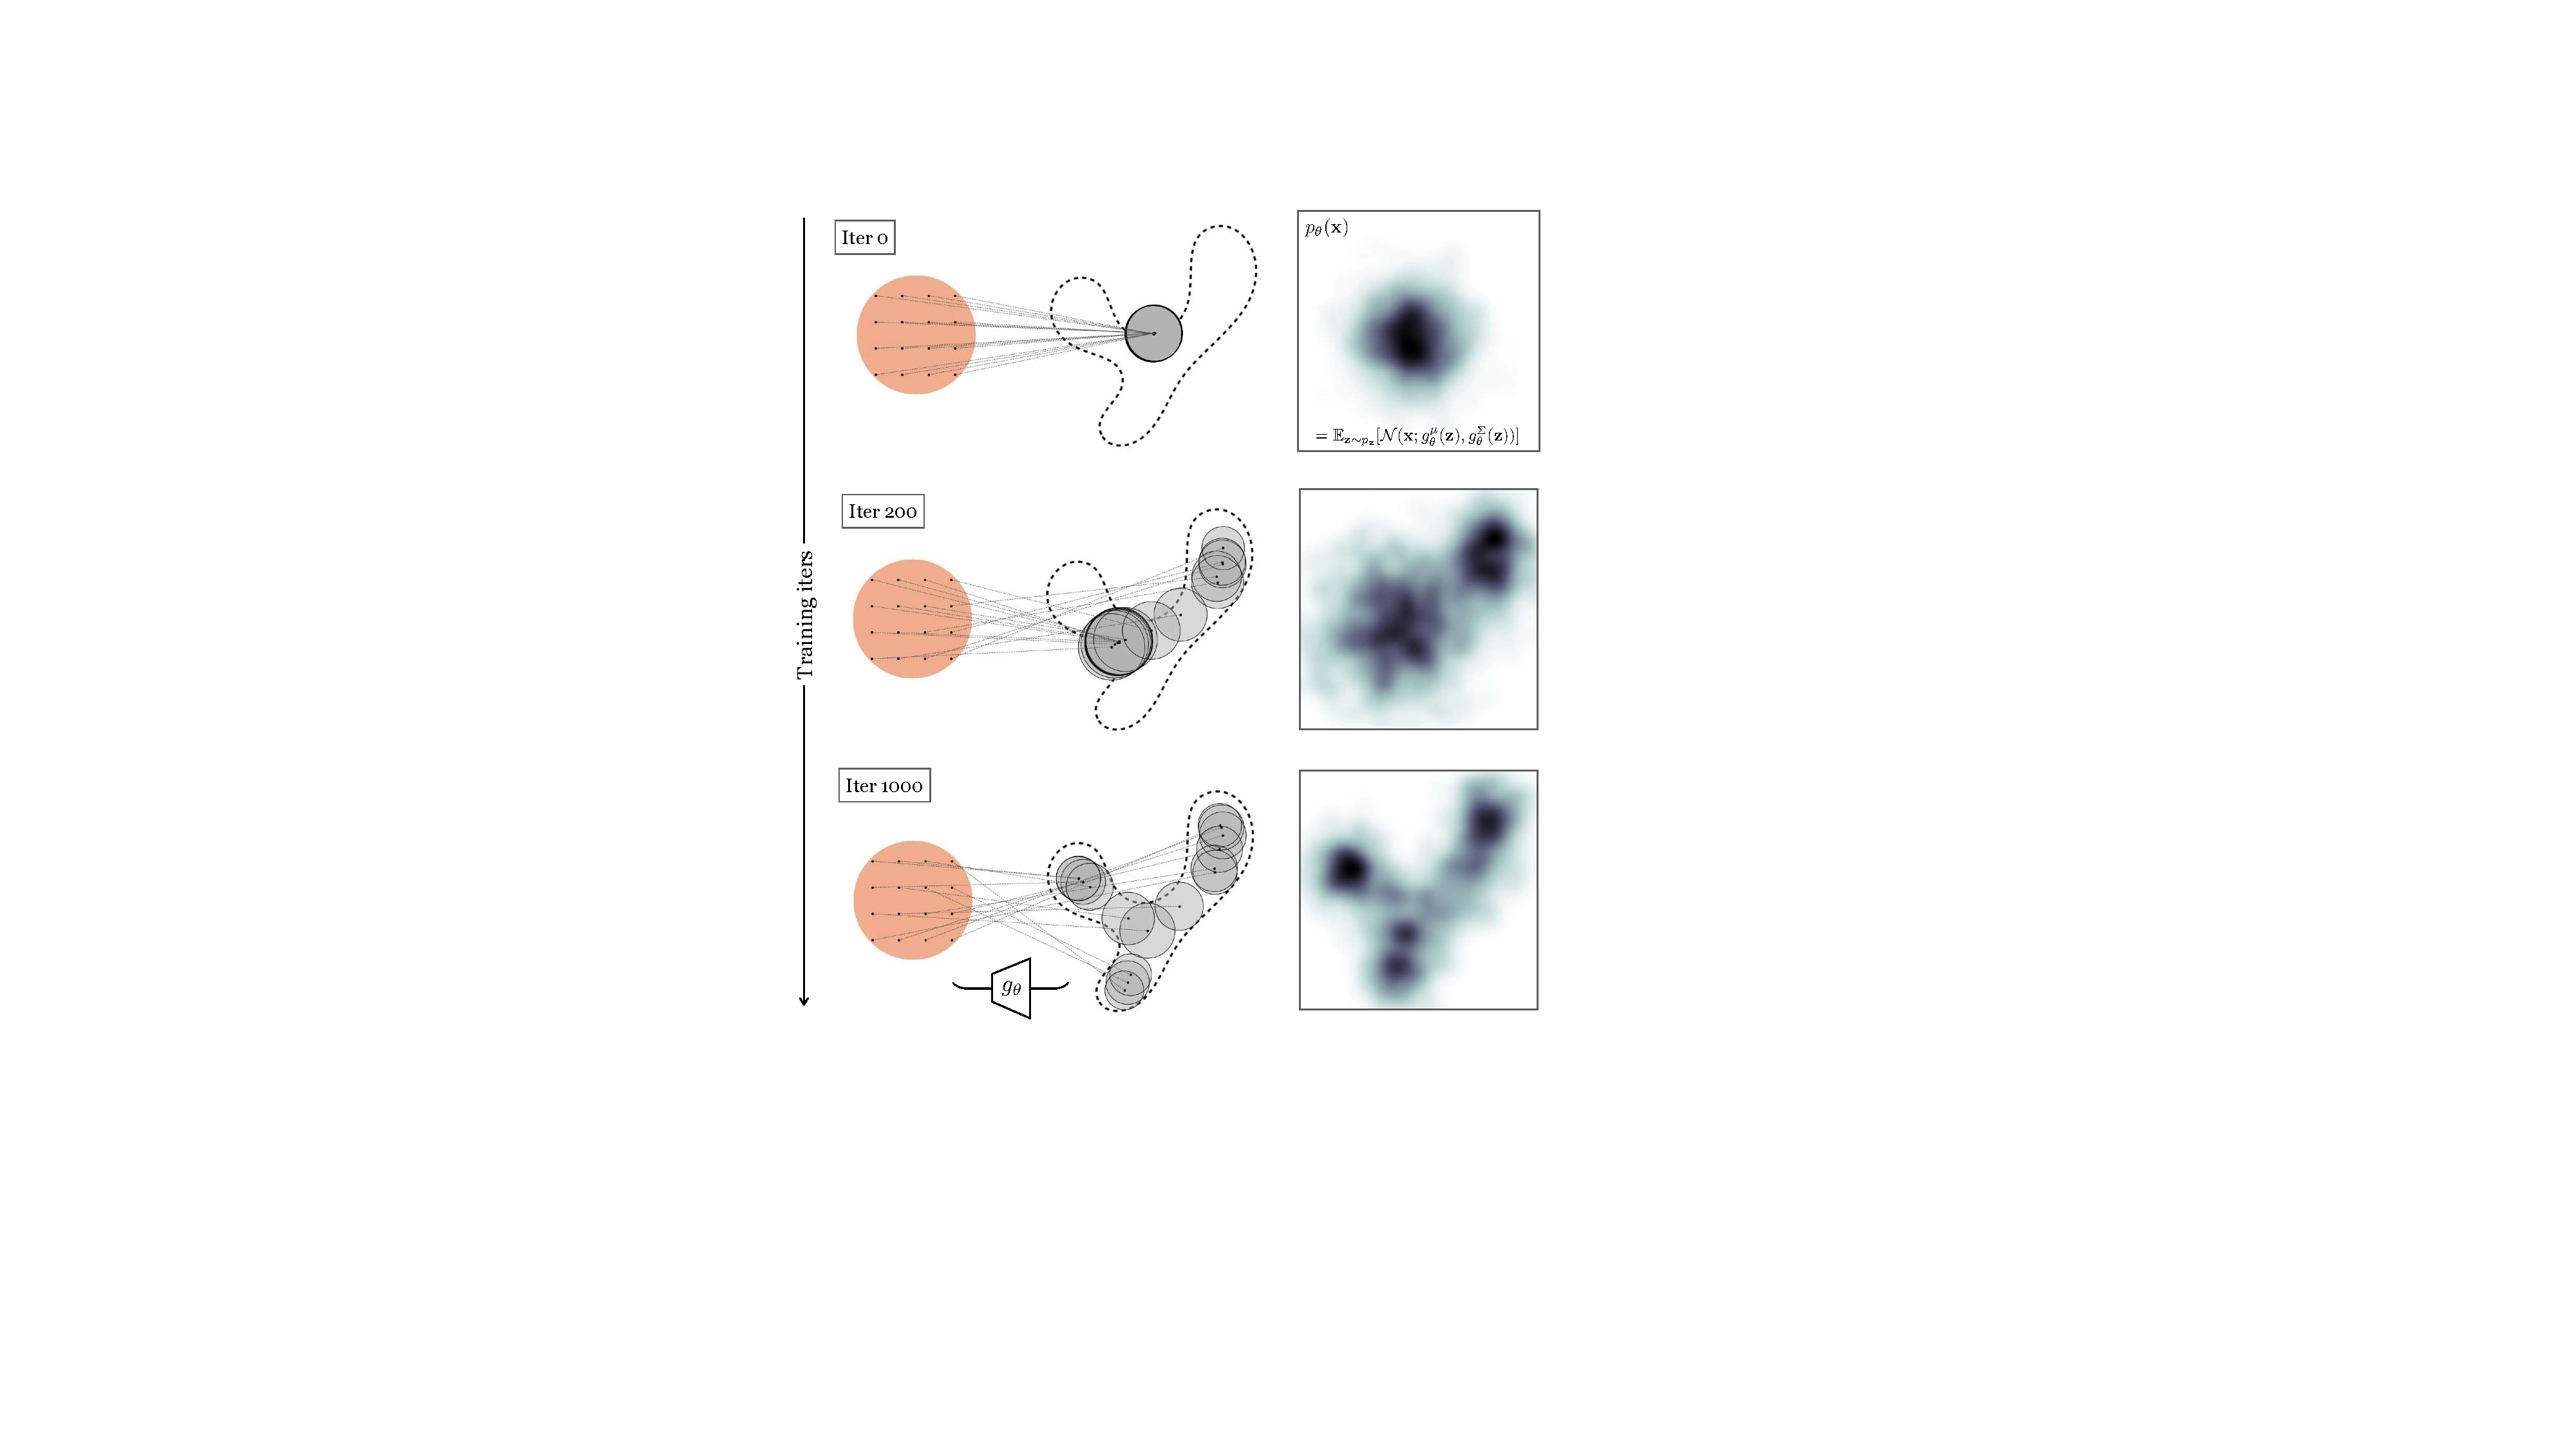
\includegraphics[width=0.7\linewidth]{./figures/generative_modeling_and_representation_learning/IGMM_training_iters.pdf}
    }
    \caption{Fitting an infinite mixture of Gaussians whose means and variances are parameterized by a generator function $g_{\theta}$.}
    \label{fig:generative_modeling_and_representation_learning:IGMM_training_iters}
\end{figure}

%[Show snap shots of mapping over training iterations, along with KDE density underneath? and on right show likelihood (ELBO?)]


% We remark that Eqn. \ref{eqn:generative_modeling_and_representation_learning:vae_learning_problem1} has an especially simple form if we set $M=1$ and fix $\mathbf{\Sigma} = \mathbf{I}$. In this case we are only learning the means of the Gaussians (this is just a less expressive hypothesis space, in which we model the distribution as an infinite mixture of istropic, unit-variance Gaussians):
% \begin{align}
%     \theta^* = \argmin_{\theta} \sum_{i=1}^N \norm{\mathbf{x}^{(i)} - g_{\theta}^{\mu}(\mathbf{z}^{(1)})}_2^2
% \end{align}
% In this form we have what looks like a regression problem: minimize the $L_2$ reconstruction error between a data point and a ``prediction" of that point. Keep this connection in mind, we will be returning to it shortly.

\subsubsection{Trick 2: Efficient approximation via importance sampling}
The previous trick works decently for modeling low-dimensional distributions. Unfortunately, this approach does not scale well to high-dimensions. The reason is that in order for our Monte Carlo estimate of the integral to be accurate, we may need many samples from $p_{\mathbf{z}}$, and the higher the dimensionality of $\mathbf{z}$, the more samples we will typically need.
%from a large portion of the density of $p_{\mathbf{z}}$; for high-dimensional $\mathbf{z}$ this means we may need a very large number of samples $M$. 

Can we come up with a more efficient way of approximating the integral in \eqn{\ref{eqn:generative_models_and_representation_learning:vae_likelihood}}? Let's start by writing out the sum from \eqn{\ref{eqn:generative_models_and_representation_learning:vae_likelihood_monte_carlo_estimate}} more explicitly:
\begin{align}
    p_{\theta}(\mathbf{x}) &\approx \frac{1}{M} (p_{\theta}(\mathbf{x} \given \mathbf{z}^{(1)}) + p_{\theta}(\mathbf{x} \given \mathbf{z}^{(2)}) + p_{\theta}(\mathbf{x} \given \mathbf{z}^{(3)}) + \ldots)
\end{align}
In general, some of the terms $p_{\theta}(\mathbf{x} \given \mathbf{z}^{(j)})$ will be larger than others. In fact, in our example in \fig{\ref{fig:generative_modeling_and_representation_learning:IGMM_training_iters}}, \textit{most} of these terms are near zero. This is because, to maximize likelihood, the model spread out the Gaussians so that each places high density on a different part of the data distribution. A datapoint $\mathbf{x}$ will only have substantial probability under the Gaussians whose means are near $\mathbf{x}$. 

Consider the example in \fig{\ref{fig:generative_modeling_and_representation_learning:vae_importance_sampling1}}, where we are trying to esimate the probability of the point $\mathbf{x}$ (blue circle). 
\begin{figure}[h!]
    \centerline{
    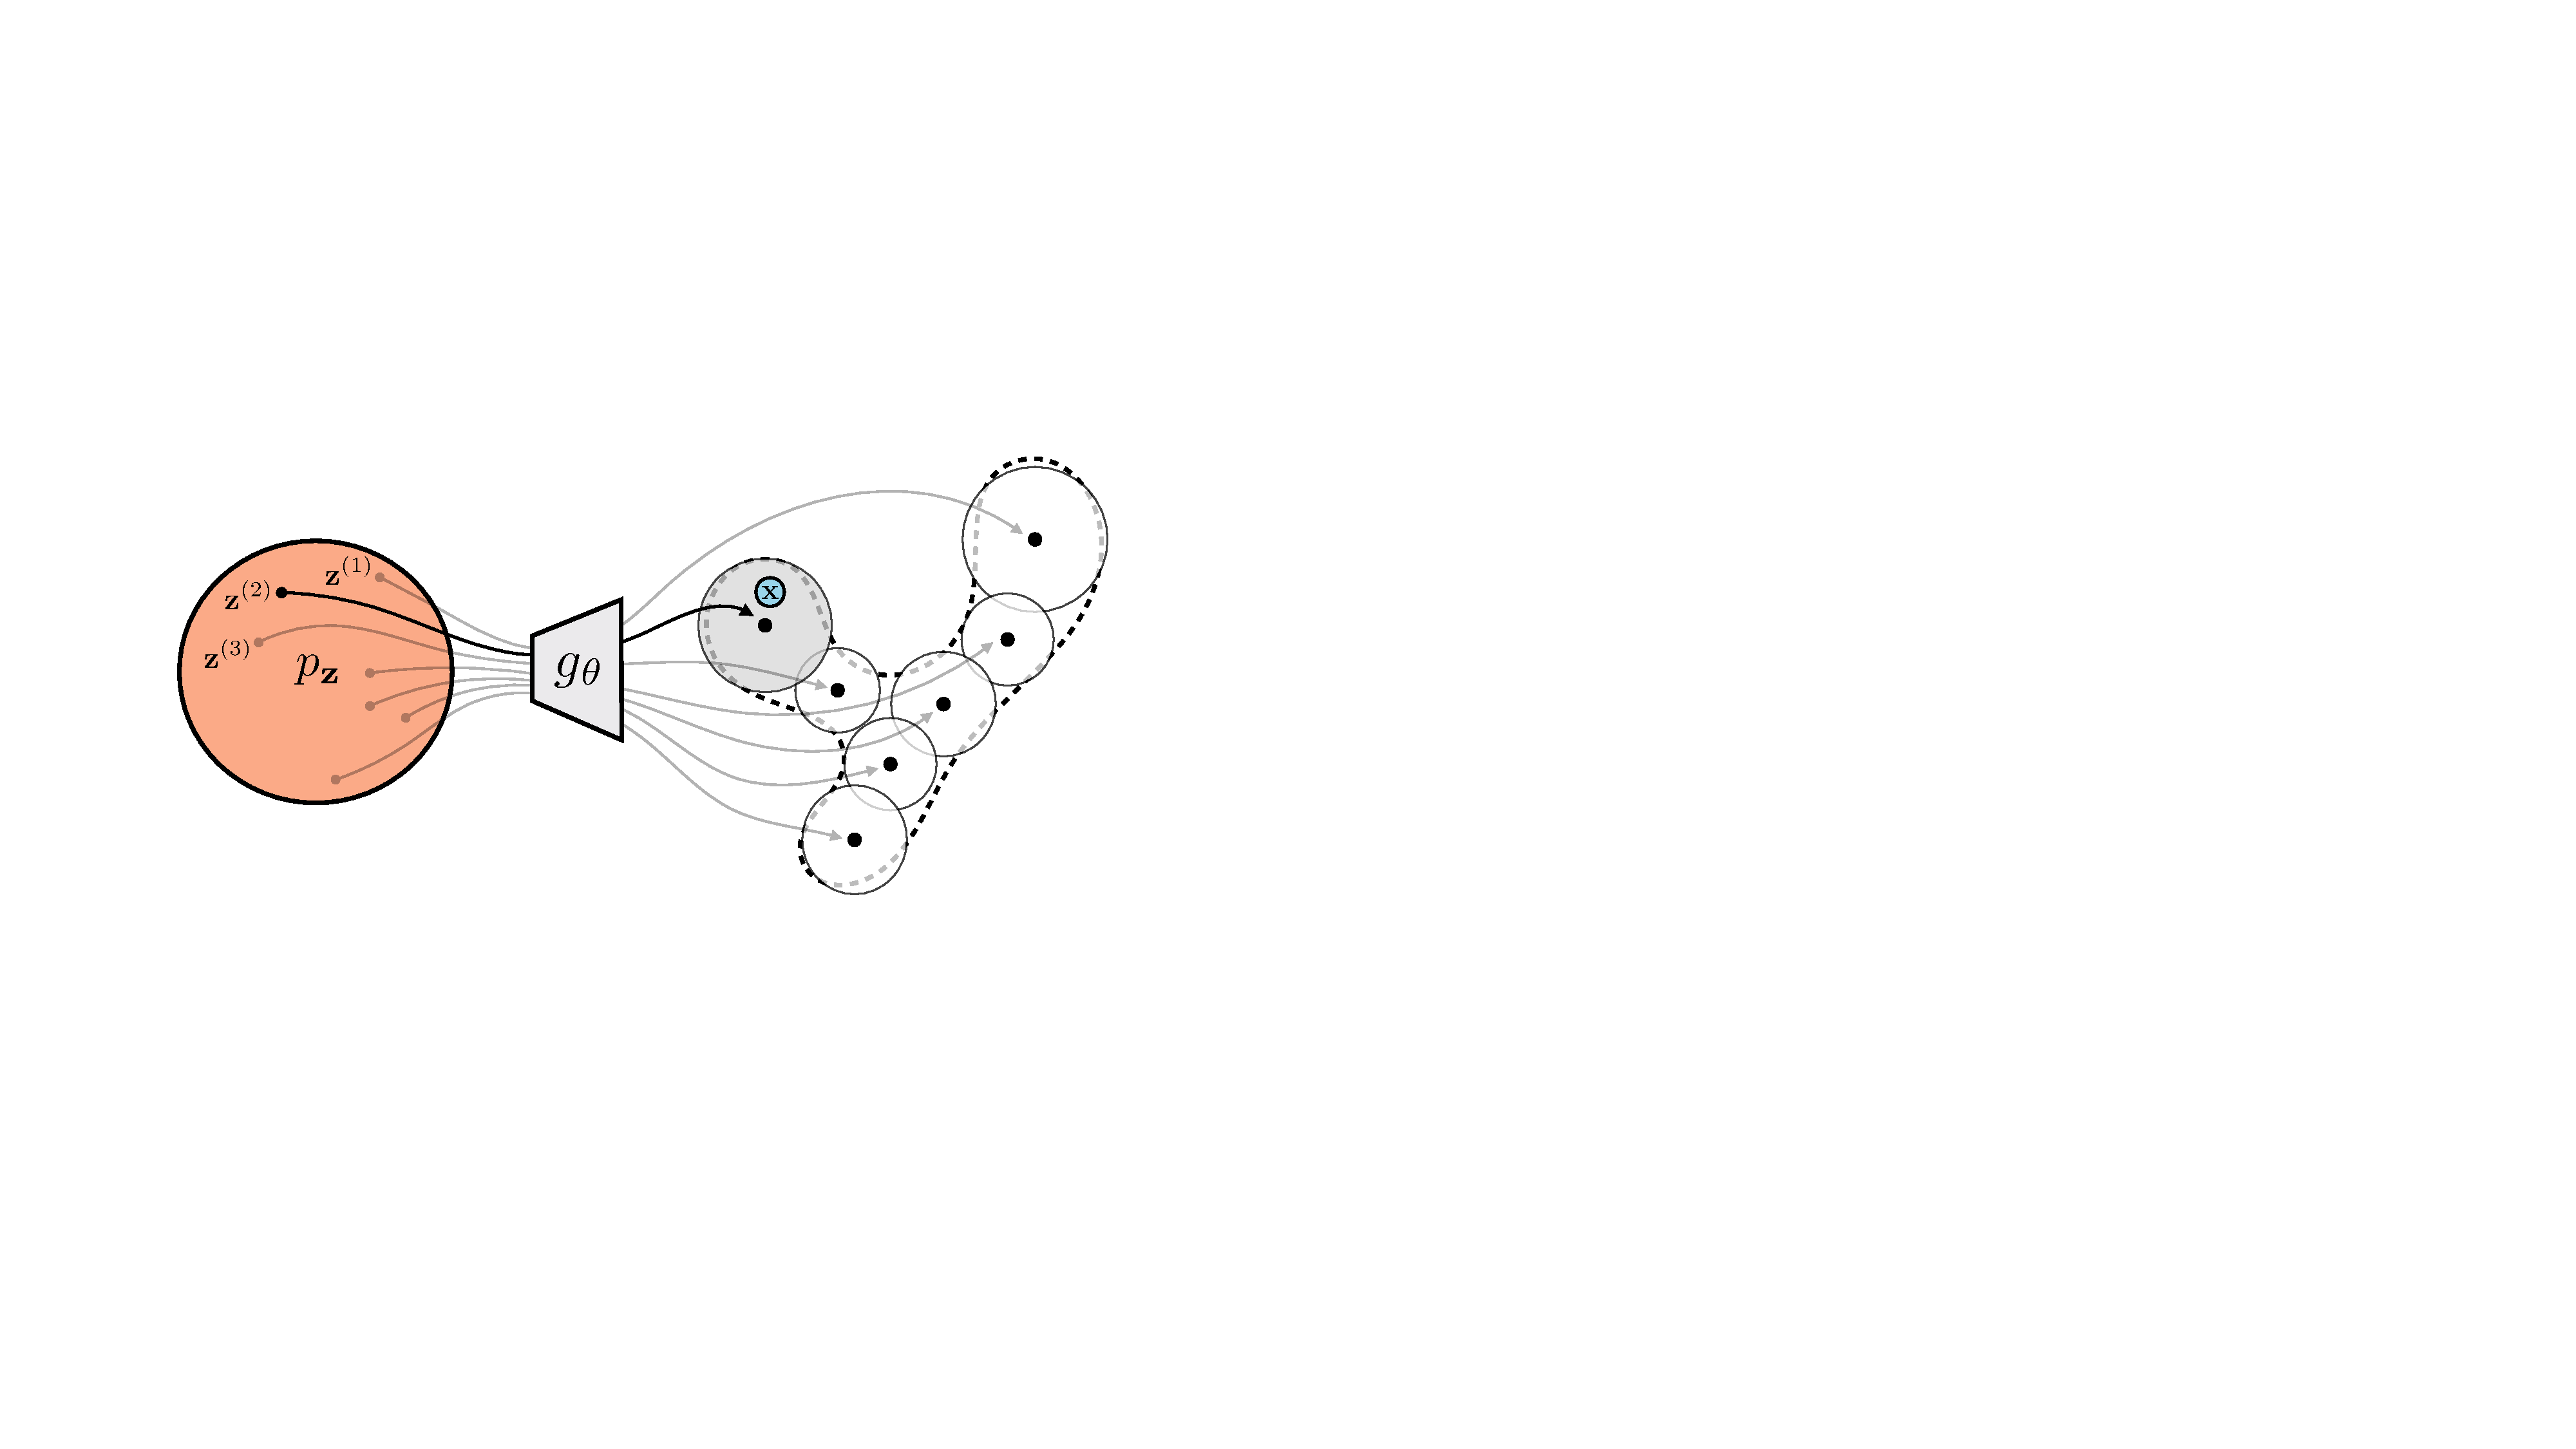
\includegraphics[width=0.5\linewidth]{./figures/generative_modeling_and_representation_learning/vae_importance_sampling1.pdf}
    }
    \caption{To estimate $p_{\theta}(\mathbf{x})$ we only need to consider the Gaussian components (gray circles) that place significant probability on $\mathbf{x}$.}
    \label{fig:generative_modeling_and_representation_learning:vae_importance_sampling1}
\end{figure}
The mixture components are shaded according to the probability they assign to $\mathbf{x}$. Almost all are so far from $\mathbf{x}$ that we have:
\begin{align}
    p_{\theta}(\mathbf{x}) &\approx \frac{1}{M} (0 + p_{\theta}(\mathbf{x} \given \mathbf{z}^{(2)}) + 0 + \ldots)
\end{align}
If we had \textit{only} sampled $\mathbf{z}^{(2)}$, we would have had almost as good an estimate!
%where $\mathbf{z}^{(*)}$ is the sampled $\mathbf{z}$ for which $g_{\theta}^{\mu}(\mathbf{z})$ is closest to $\mathbf{x}$, in $L_2$ distance.

This brings us to the second trick of VAEs: when approximating the likelihood integral for $p_{\theta}(\mathbf{x})$, try to only sample $\mathbf{z}$ values that place high probability on $\mathbf{x}$, that is, those $\mathbf{z}$ values for which $p_{\theta}(\mathbf{x} \given \mathbf{z})$ is large. Then, a few samples will suffice to well approximate the entire expectation. This trick is called \index{Importance sampling}\textbf{importance sampling}. It is a general trick for approximating expectations. Rather than sampling $\mathbf{z}^{(i)} \sim p_{\mathbf{z}}$, we sample from some other density $\mathbf{z}^{(i)} \sim q_{\mathbf{z}}$, and multiply by a correction factor $\frac{p_{\mathbf{z}}(\mathbf{z})}{q_{\mathbf{z}}(\mathbf{z})}$ to account for the fact that we are sampling from a biased distribution:
\begin{align}
p_{\theta}(\mathbf{x}) &= \mathbb{E}_{\mathbf{z}\sim p_{\mathbf{z}}}\Big[p_{\theta}(\mathbf{x} \given \mathbf{z})\Big]
= \int_{\mathbf{z}} p_{\mathbf{z}}(\mathbf{z}) p_{\theta}(\mathbf{x} \given \mathbf{z}) d\mathbf{z}
= \int_{\mathbf{z}} q_{\mathbf{z}}(\mathbf{z})\frac{p_{\mathbf{z}}(\mathbf{z})}{q_{\mathbf{z}}(\mathbf{z})} p_{\theta}(\mathbf{x} \given \mathbf{z}) d\mathbf{z}\\
&= \mathbb{E}_{\mathbf{z}\sim q_{\mathbf{z}}}\Big[\frac{p_{\mathbf{z}}(\mathbf{z})}{q_{\mathbf{z}}(\mathbf{z})} p_{\theta}(\mathbf{x} \given \mathbf{z})\Big]\label{eqn:generative_modeling_and_representation_learning:vae_learning_problem2}
%&\approx \frac{1}{N} \sum_{i=1}^N \frac{p_{\mathbf{z}}(\mathbf{z}^{(i)})}{q_{\psi}(\mathbf{z}^{(i)})} p_{\theta}(\mathbf{x} | \mathbf{z}^{(i)}), \quad \mathbf{z}^{(i)} \sim q_{\psi} \label{eqn:generative_models_and_representation_learning:vae_importance_sampling}
\end{align}
Using the intuition we developed previously, the distribution $q$ we would really like to sample from is the one whose samples maximize $p_{\theta}(\mathbf{x} \given \mathbf{z})$. It turns out that the optimal distribution is $q^* = p_{\theta}(Z \given \mathbf{x})$.\footnote{See chapter 9, setion 1 of \cite{mcbook} for a proof that $q^*(\mathbf{z}) \propto \lvert p_{\theta}(\mathbf{x} \given \mathbf{z}) \rvert p_{\mathbf{z}}(\mathbf{z})$, from which it then follows that $q^*(\mathbf{z}) \propto p_{\theta}(\mathbf{x} \given \mathbf{z})p_{\mathbf{z}}(\mathbf{z}) = p_{\theta}(\mathbf{x}, \mathbf{z}) \propto p_{\theta}(\mathbf{z} \given \mathbf{x})$, yielding our result.} This distribution minimizes the expected error between a Monte Carlo estimate of the expectation and its true value (i.e., minimizes the variance of our Monte Carlo estimator). The intuition is that $p_{\theta}(Z \given \mathbf{x})$ is precisely a prediction of which $\mathbf{z}$ values are most likely to have generated the observed $\mathbf{x}$. The optimal importance sampling way to estimate the likelihood of a datapoint will therefore look like this:
\begin{align}
    &p_{\theta}(\mathbf{x}) \approx \frac{1}{M} \sum_{j=1}^M\frac{p_{\mathbf{z}}(\mathbf{z}^{(j)})}{p_{\theta}(\mathbf{z}^{(j)} \given \mathbf{x})} p_{\theta}(\mathbf{x} \given \mathbf{z}^{(j)}) \quad\quad \triangleleft \quad\text{Optimal importance sampling}\label{eqn:generative_models_and_representation_learning:vae_importance_sampling}\\
    &\quad\quad \mathbf{z}^{(j)} \sim p_{\theta}(Z \given \mathbf{x}) \nonumber
\end{align}
Visually, rather than sampling from all over $p_{\mathbf{z}}$ and wasting samples on regions that place nearly zero likelihood on the data, we focus our sampling on just the region that places high likelihood on the data, and we can get then away with far
fewer samples to well approximate the data likelihood, as indicated \fig{\ref{fig:generative_modeling_and_representation_learning:vae_importance_sampling2}}.
\begin{figure}[h!]
    \centerline{
    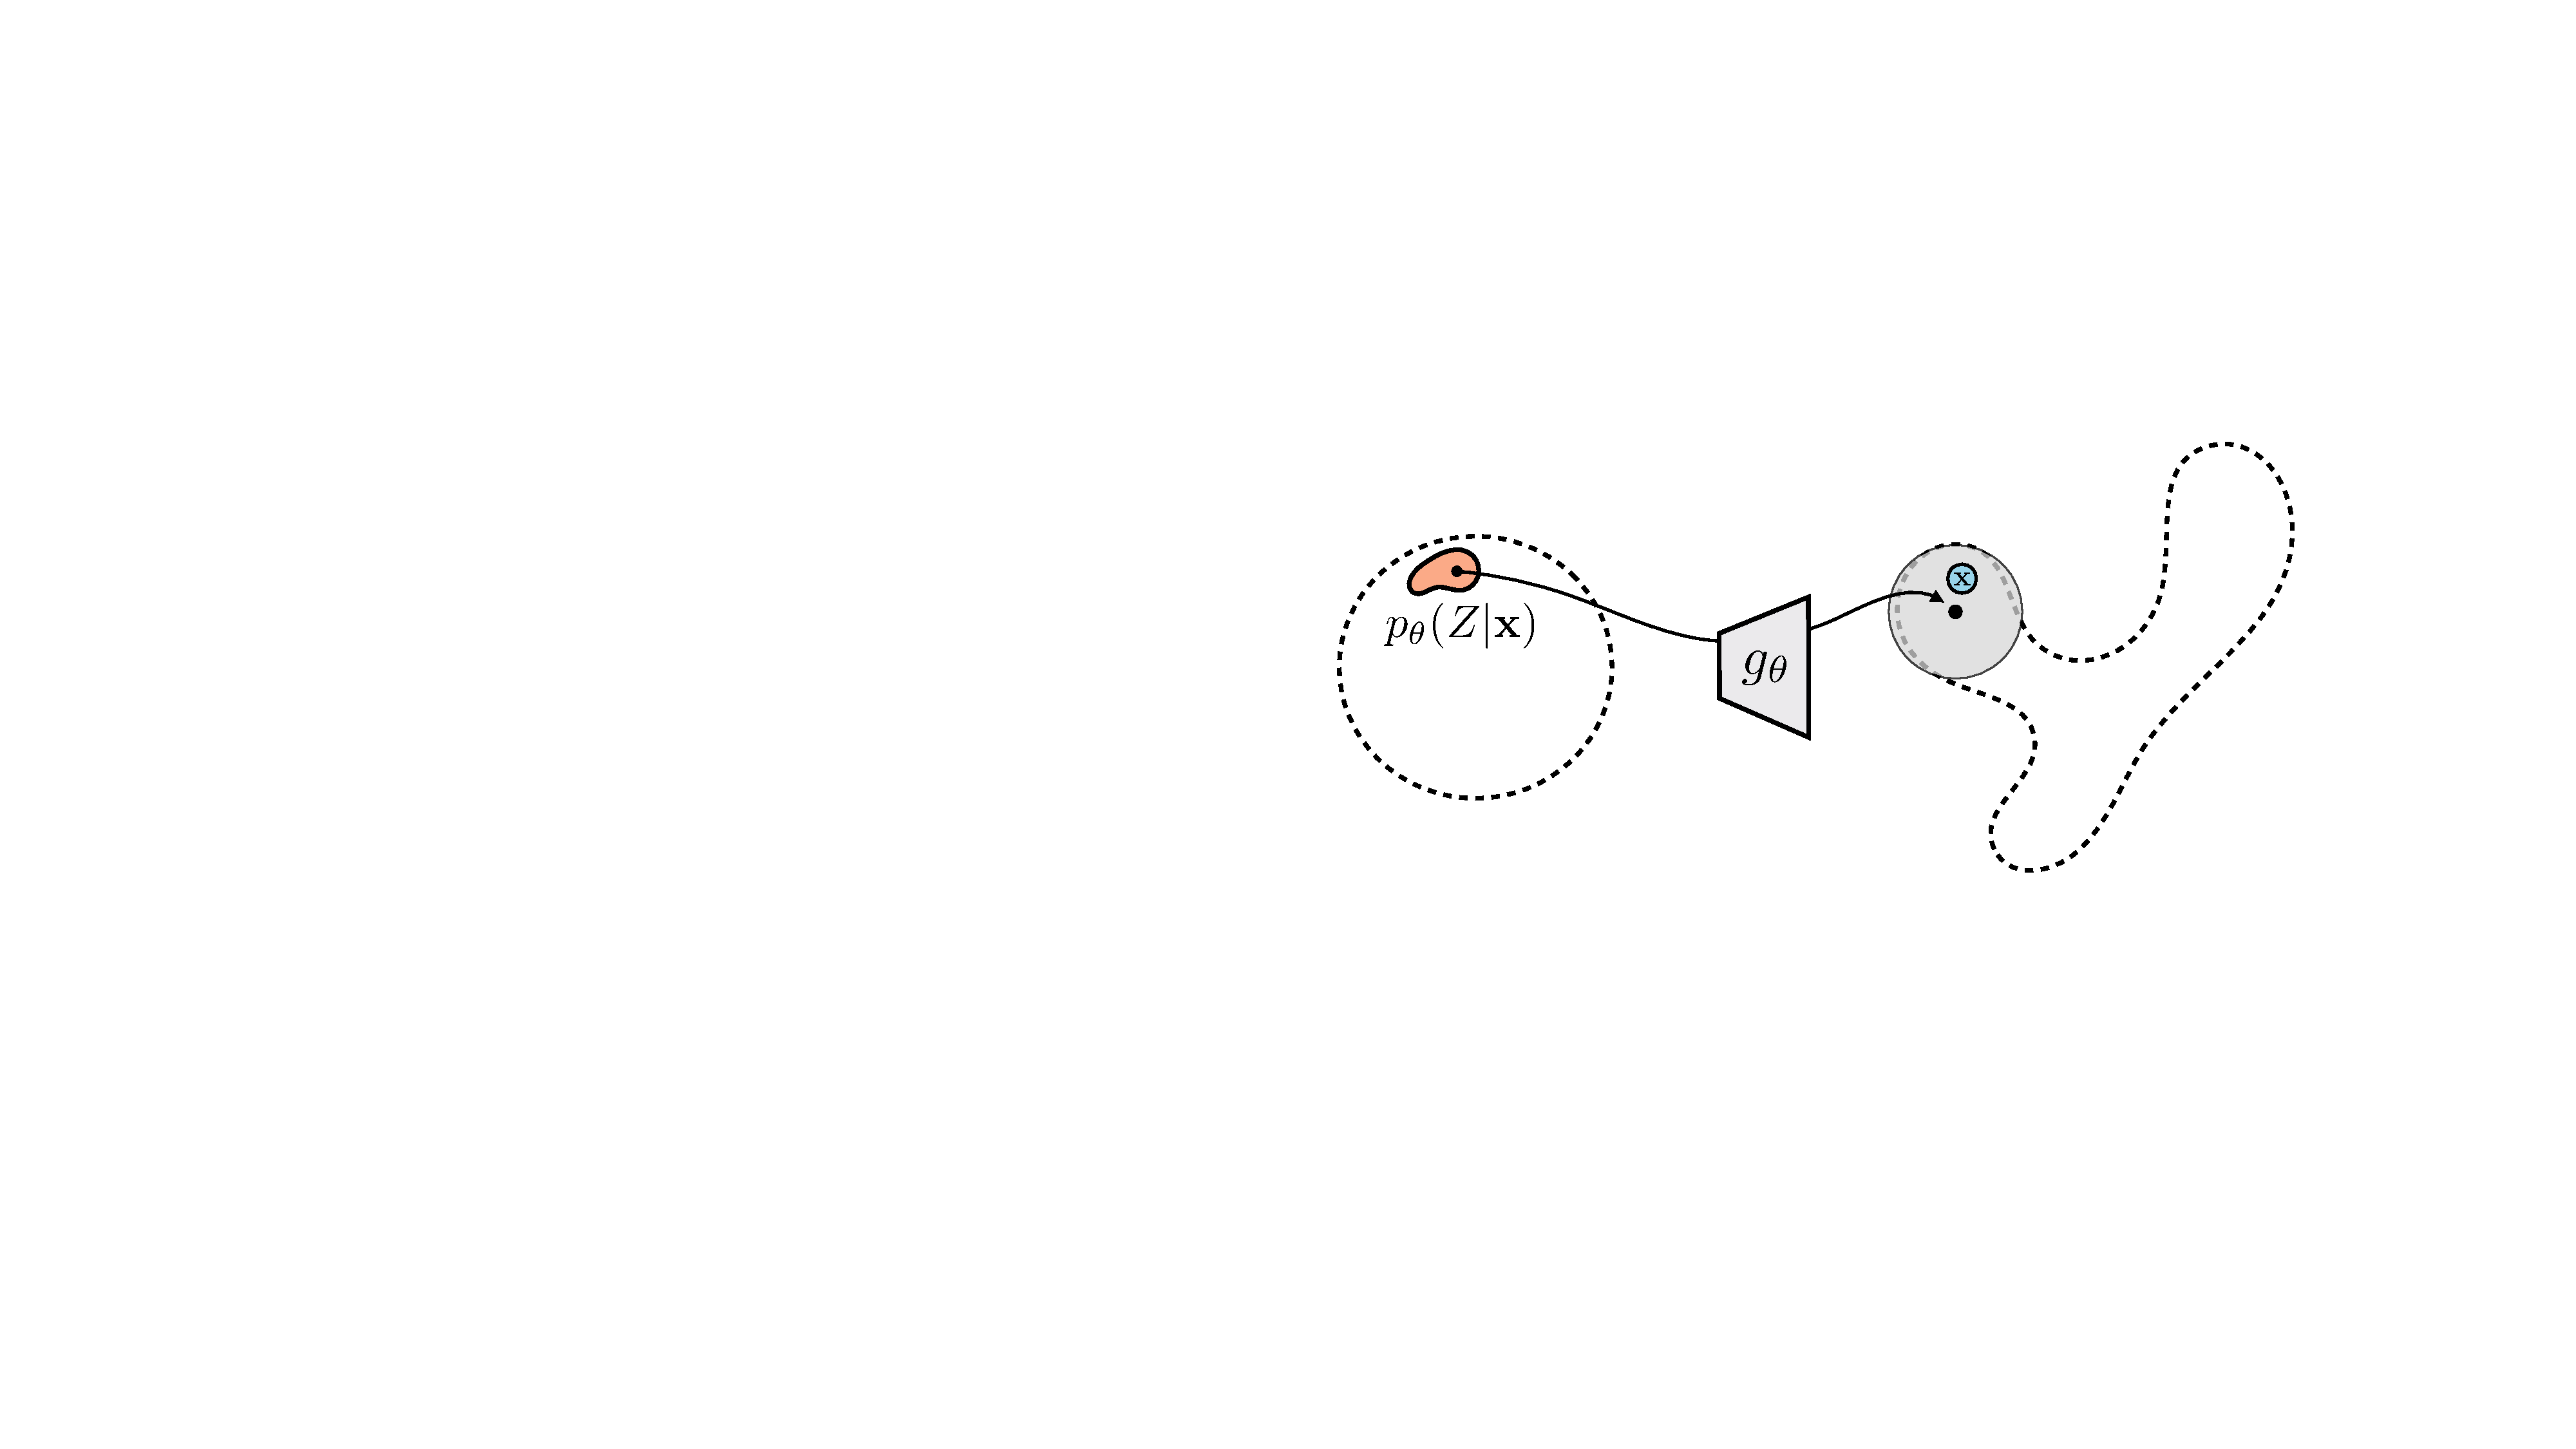
\includegraphics[width=0.5\linewidth]{./figures/generative_modeling_and_representation_learning/vae_importance_sampling2.pdf}
    }
    \caption{Optimal importance sampling estimates $p_{\theta}(\mathbf{x})$ by drawing samples from $p_{\theta}(Z \given \mathbf{x})$.}
    \label{fig:generative_modeling_and_representation_learning:vae_importance_sampling2}
\end{figure}

%Now the only question is what's the best $q$ to sample from. We want it to be a distribution over $\mathbf{z}$ such that samples from it tend to have high $p_{\theta}(\mathbf{x} | \mathbf{z})$. Intuitively, $p_{\theta}(\mathbf{z} | \mathbf{x})$ is exactly such a distribution, as it tells us ``given this $\mathbf{x}$, what do we believe is the $\mathbf{z}$ that generated it?" It turns out that setting XX = XX is indeed optimal: this is the q that minimizes YY (see a proof in XX).

%As can be seen if you write out the integral, the two expectations above are \textit{exactly equal}, and this is true for \textit{any} distribution $q_{\psi}$. Intuitively, as we alluded to above, we want the samples from $q_{\psi}$ to be the dominate terms in the sum in Eqn. \ref{eqn:generative_models_and_representation_learning:vae_likelihood_monte_carlo_estimate}, so that only a few samples will suffice to well approximate the integral. It turns out that the best $q_{\psi}$ may be different for different values of $\mathbf{x}$; since any pdf $q_{\psi}$ is valid we can use a different one for approximating the expectation in Eqn. \ref{eqn:generative_models_and_representation_learning:vae_likelihood2} for each different value of $\mathbf{x}$. Since each $q_{\psi}$ is a density, we can naturally represent a different $q_{\psi}$ for each $\mathbf{x}$ as a conditional density $q_{\psi}(\mathbf{z} | \mathbf{x})$.

%Now we could pick any conditional distribution $q_{\psi}(\mathbf{z} | \mathbf{x})$ but which is the best? More precisely, what is the best distribution $q_{\psi}$ to sample from in order that the approximation in Eqn. \ref{eqn:generative_models_and_representation_learning:vae_importance_sampling} is expected to vary from the true value as little as possible? Based on the intuitions above, we want it to be the distribution over $\mathbf{z}$ such that samples from it have high $p_{\theta}(\mathbf{x} | \mathbf{z})$. 

%The theory of importance sampling tells us that the answer is $q_{\psi}^*(\mathbf{z} | \mathbf{x}) = p_{\theta}(\mathbf{z}|\mathbf{x})$ (see XX for a proof that, under mild conditions, this is indeed the optimal $q_{\psi}$). Notice that this also justifies why we used conditioned $q_{\psi}$ on $\mathbf{x}$, since the optimal $q_{\psi}$ is different for different $\mathbf{x}$'s.%\marginnote{In a slight abuse of notation, $p_{\theta}(\mathbf{z}|\mathbf{x})$ here refers to the conditional distribution over all $\mathbf{x}$'s rather than the value of this distribution at one particular $\mathbf{x}$.}





% This idea is called {\bf importance sampling}. Rather than sampling $\mathbf{z}^{(i)} \sim p_{\mathbf{z}}$ to approximate the integral, we sample from the distribution $\mathbf{z}^{(i)} \sim q_{\psi}$, and multiply by a correction factor $\frac{p_{\mathbf{z}}(\mathbf{z})}{q_{\psi}(\mathbf{z})}$ to account for the fact that we are sampling from a biased distribution:
% \begin{align}
% p_{\theta}(\mathbf{x}) &= \mathbb{E}_{\mathbf{z}\sim p_{\mathbf{z}}}\Big[p_{\theta}(\mathbf{x} | \mathbf{z})\Big] \label{eqn:generative_models_and_representation_learning:vae_likelihood2}\\
% &= \mathbb{E}_{\mathbf{z}\sim q_{\psi}}\Big[\frac{p_{\mathbf{z}}(\mathbf{z})}{q_{\psi}(\mathbf{z})} p_{\theta}(\mathbf{x} | \mathbf{z})\Big]\\
% &\approx \frac{1}{N} \sum_{i=1}^N \frac{p_{\mathbf{z}}(\mathbf{z}^{(i)})}{q_{\psi}(\mathbf{z}^{(i)})} p_{\theta}(\mathbf{x} | \mathbf{z}^{(i)}), \quad \mathbf{z}^{(i)} \sim q_{\psi} \label{eqn:generative_models_and_representation_learning:vae_importance_sampling}
% \end{align}
% As can be seen if you write out the integral, the two expectations above are \textit{exactly equal}, and this is true for \textit{any} distribution $q_{\psi}$. Intuitively, as we alluded to above, we want the samples from $q_{\psi}$ to be the dominate terms in the integral in Eqn. \ref{eqn:generative_models_and_representation_learning:vae_likelihood}, so that only a few samples will suffice to well approximate the integral. It turns out that the best $q_{\psi}$ may be different for different values of $\mathbf{x}$; since any pdf $q_{\psi}$ is valid we can use a different one for approximating the expectation in Eqn. \ref{eqn:generative_models_and_representation_learning:vae_likelihood2} for each different value of $\mathbf{x}$. Since each $q_{\psi}$ is a density, we can naturally represent a different $q_{\psi}$ for each $\mathbf{x}$ as a conditional density $q_{\psi}(\mathbf{z} | \mathbf{x})$.


\subsubsection{Trick 3: Variational inference to approximate the sampling distribution}

Now we know what distribution we \textit{should} be sampling $\mathbf{z}$ from: $p_{\theta}(Z \given \mathbf{x})$. The only remaining problem is that this distribution may be complicated and hard to sample from. \marginnote{Remember, we have defined simple forms for only $p_{\theta}(X \given \mathbf{z})$ and $p_{\mathbf{z}}$ (both are Gaussians), but this does not mean $p_{\theta}(Z \given \mathbf{x})$ has a simple form.}[-1.0cm]
Sampling from arbitrary distributions is a standard topic in statistics, and many algorithms have been proposed, including the Markov chain Monte Carlo methods we encountered in previous chapters. VAEs use a strategy called \index{Variational inference}\textbf{variational inference}.\marginnote{The name \textit{variational} comes from the ``calculus of variations,'' which studies functionals (functions of functions). Integrals of probability densities are functionals. Variational inference is commonly (but not always) used to approximate densities expressed as the integral of some other densities, hence functionals, hence the name variational.}[7cm]

The idea of variational inference is to approximate an intractable density $p$ by finding the nearest density in a tractable family $q_{\psi}$, parameterized by $\psi$. In VAEs, we approximate our ideal importance density $p_{\theta}(Z \given \mathbf{x})$ with a $q_{\psi}$ in a family we can efficiently sample from; the most common choice is to again use a Gaussian, conditioned on $\mathbf{x}$: $q_{\psi} = \mathcal{N}(f_{\psi}^{\mu}(\mathbf{x}), f_{\psi}^{\Sigma}(\mathbf{x}))$. The $f_{\psi}$ is a function that maps from $\mathbf{x}$ to parameters of a distribution over $\mathbf{z}$; in other words, $f_{\psi}$ is a probabilistic encoder! This function is shown next in \fig{\ref{fig:generative_modeling_and_representation_learning:VAE_encoder}}:
\begin{figure}[h!]
    \centerline{
    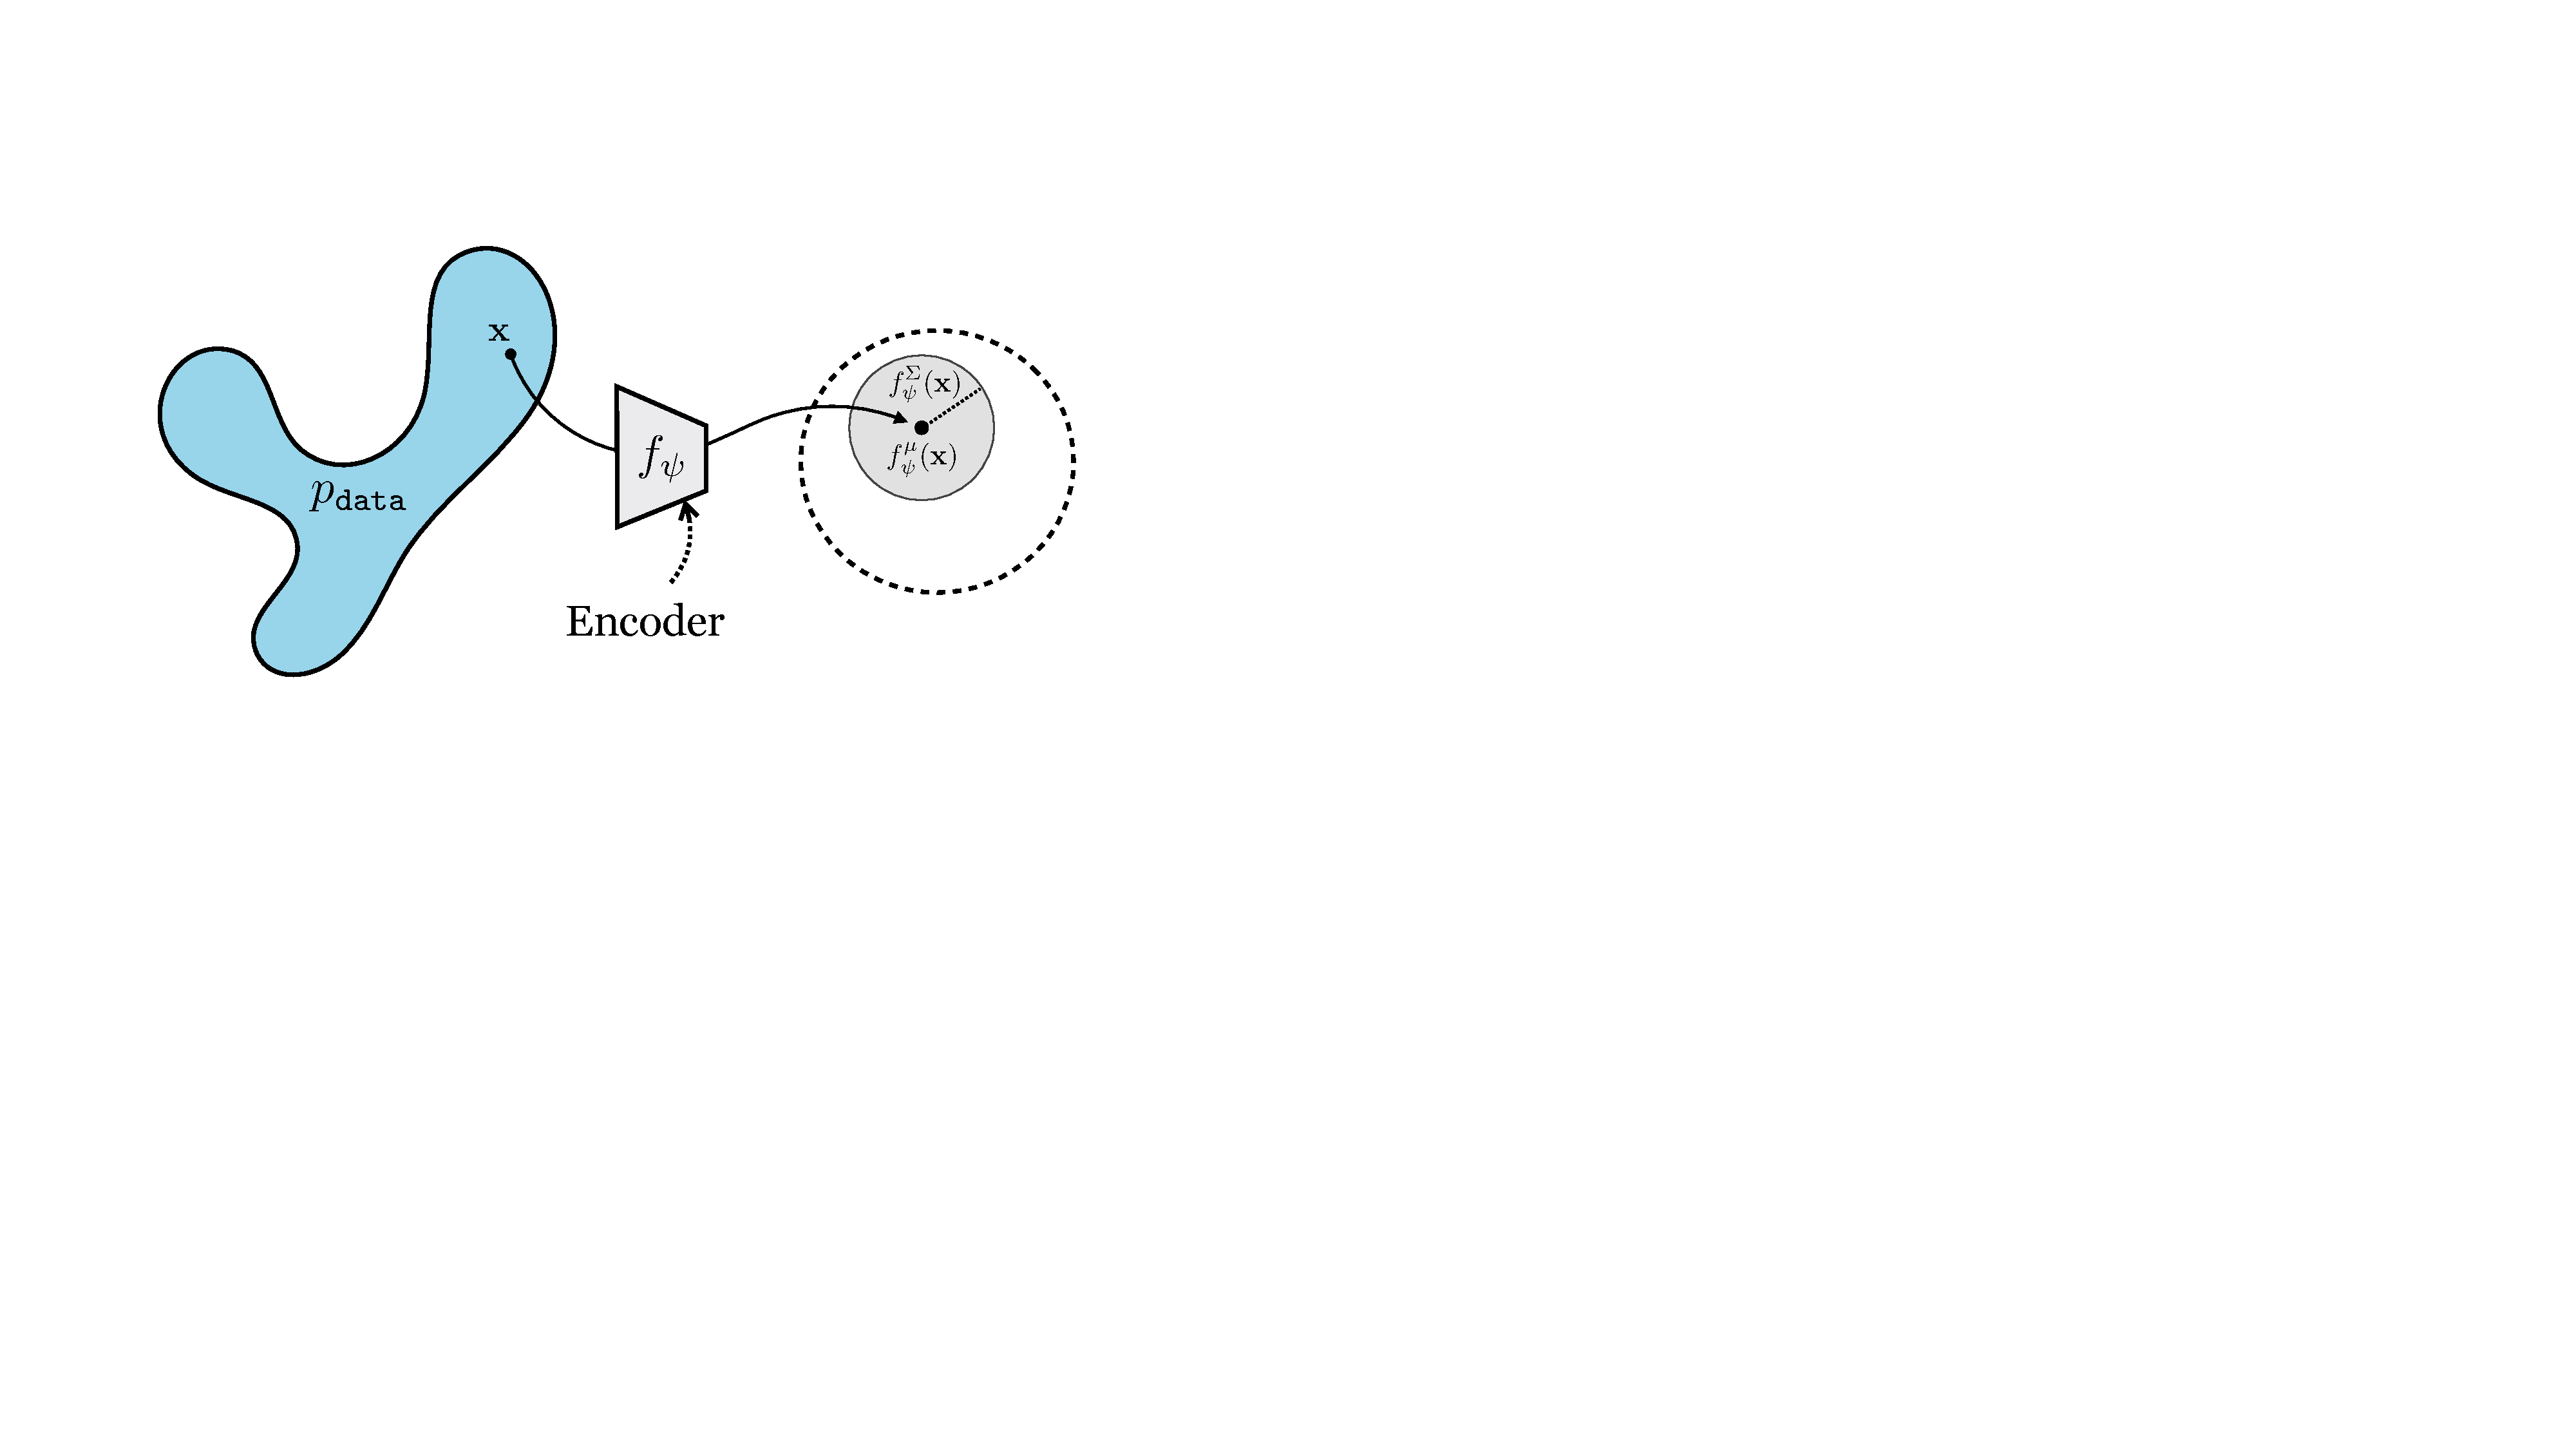
\includegraphics[width=0.55\linewidth]{./figures/generative_modeling_and_representation_learning/VAE_encoder.pdf}
    }
    \caption{A VAE's encoder, $f_{\psi}$, models $p(Z \given \mathbf{x})$ as a Gaussian parameterized by $f_{\psi}(\mathbf{x})$.}
    \label{fig:generative_modeling_and_representation_learning:VAE_encoder}
\end{figure}

It will turn out that $f$ indeed plays the role of the encoder in the VAE, while $g$ plays the role of the decoder.

We want $q_{\psi}$ to be the best approximation of $p_{\theta}(Z \given \mathbf{x})$, so our goal will be to choose the $q_{\psi}$ that minimizes the Kullback-Leibler (KL) divergence between these two distributions. We could have chosen other divergences or notions of approximation, but we will see that using the KL divergence yields some nice properties. We will call the objective for $q_{\psi}$ as $J_{q}$, which we will define as the negative KL-divergence, so our goal is to maximize this quantity. Using the definition of KL-divergence, we can expand this objective as follows: %\marginnote{Recall that $H = \mathbb{E}_p[\log p]$ is the entropy of a distribution $p$.}[1.8cm]
\begin{align}
    J_q(\mathbf{x},\psi) &= -\KLdiv{q_{\psi}(Z \given \mathbf{x})}{p_{\theta}(Z \given \mathbf{x})}\\
    &= -\mathbb{E}_{\mathbf{z} \sim q_{\psi}(Z \given \mathbf{x})}[ \log q_{\psi}(\mathbf{z} \given \mathbf{x}) - \log p_{\theta}(\mathbf{z} \given \mathbf{x})]\\
    &= -\mathbb{E}_{\mathbf{z} \sim q_{\psi}(Z \given \mathbf{x})}[ \log q_{\psi}(\mathbf{z} \given \mathbf{x}) - \log p_{\theta}(\mathbf{x} \given \mathbf{z}) - \log p_{\mathbf{z}}(\mathbf{z}) + \log p_{\theta}(\mathbf{x})]\\
    &= \mathbb{E}_{\mathbf{z} \sim q_{\psi}(Z \given \mathbf{x})}[ -\log q_{\psi}(\mathbf{z} \given \mathbf{x}) + \log p_{\theta}(\mathbf{x} \given \mathbf{z}) + \log p_{\mathbf{z}}(\mathbf{z})] - \log p_{\theta}(\mathbf{x})
    %&= H(q_{\psi}) - \mathbb{E}_{\mathbf{z} \sim q_{\psi}(Z|\mathbf{x})}[ \log p_{\theta}(\mathbf{z} | \mathbf{x})]\\
    %&= H(q_{\psi}) - \mathbb{E}_{\mathbf{z} \sim q_{\psi}(Z|\mathbf{x})}[ \log p_{\theta}(\mathbf{z}, \mathbf{x}) - \log p_{\theta}(\mathbf{x})] \\
    %&= H(q_{\psi}) - \mathbb{E}_{\mathbf{z} \sim q_{\psi}(Z|\mathbf{x})}[ \log p_{\theta}(\mathbf{x} | \mathbf{z}) + \log p_{\mathbf{z}}(\mathbf{z})] + \mathbb{E}_{\mathbf{z} \sim q_{\psi}(Z|\mathbf{x})}[\log p_{\theta}(\mathbf{x})] \\
    %&= H(q_{\psi}) - \mathbb{E}_{\mathbf{z} \sim q_{\psi}(Z|\mathbf{x})}[ \log p_{\theta}(\mathbf{x} | \mathbf{z}) + \log p_{\mathbf{z}}(\mathbf{z})] + \log p_{\theta}(\mathbf{x})
    %&= \argmin_{q_\psi} H(q_{\psi}) - \mathbb{E}_{\mathbf{z} \sim q_{\psi}(Z|\mathbf{x})}[ \log p_{\theta}(\mathbf{x} | \mathbf{z}) + \log p_{\mathbf{z}}(\mathbf{z})]
\end{align}
The last line follows from the fact that $\log p_{\theta}(\mathbf{x})$ is a constant with respect to the distribution we are taking expectation over.

The learning problem for $q_{\psi}$ is to maximize $J_q$, over all images in our dataset, $\{\mathbf{x}^{(i)}\}_{i=1}^N$, with respect to parameters $\psi$. Notice that the term $\log p_{\theta}(\mathbf{x})$ is constant with respect to these parameters, so we can drop that term, yielding:
\begin{align}
    \psi^* &= \argmax_{\psi} \frac{1}{N}\sum_{i=1}^N J_q(\mathbf{x}^{(i)}, \psi)\\
    &= \argmax_{\psi} \frac{1}{N}\sum_{i=1}^N \underbrace{\mathbb{E}_{\mathbf{z} \sim q_{\psi}(Z \given \mathbf{x}^{(i)})}[ -\log q_{\psi}(\mathbf{z} \given \mathbf{x}^{(i)}) + \log p_{\theta}(\mathbf{x}^{(i)} \given \mathbf{z}) + \log p_{\mathbf{z}}(\mathbf{z})]}_{J} \label{eqn:generative_modeling_and_representation_learning:J_q}
\end{align}
Here we have defined a new cost function, $J$ (the term inside the sum in \eqn{\ref{eqn:generative_modeling_and_representation_learning:J_q}}), whose maximizer with respect to $\psi$ is the same as the maximizer for $J_q$.
%\begin{align}
%     q_{\psi}^* &= \argmin_{q_{\psi}} (H(q_{\psi}) - \mathbb{E}_{\mathbf{z} \sim q_{\psi}(Z|\mathbf{x})}[ \log p_{\theta}(\mathbf{x} | \mathbf{z}) + \log p_{\mathbf{z}}(\mathbf{z})])\\
%     &= \argmin_{q_{\psi}} (H(q_{\psi}) - \mathbb{E}_{\mathbf{z} \sim q_{\psi}(Z|\mathbf{x})}[ \log p_{\theta}(\mathbf{x} | \mathbf{z}) ] - H(q_{\psi}(Z|\mathbf{x}), p_{\mathbf{z}}))\\
%     &= \argmin_{q_{\psi}} (- \overbrace{\mathbb{E}_{\mathbf{z} \sim q_{\psi}(Z|\mathbf{x})}[ \log p_{\theta}(\mathbf{x} | \mathbf{z}) ]}^{\text{place lots of probability on $\mathbf{x}$}} - \underbrace{\KLdiv{q_{\psi}(Z | \mathbf{x})}{p_{\mathbf{z}}}}_{\text{don't deviate too much from $p_{\mathbf{z}}$}})
% \end{align}
%The text in the equation above indicates how the objective decomposes into two intuitive goals for $q_{\psi}$.

Now, let us now recall our learning problem for $p_{\theta}$, which is to maximize data log likelihood. Using importance sampling to estimate data likelihood (equation [\ref{eqn:generative_modeling_and_representation_learning:vae_learning_problem2}]), and using $q_{\psi}$ as our sampling distribution, we have that the objective for $p_{\theta}$ is to maximize the following objective $J_p$ with respect to $\theta$:
\begin{align}
    J_p(\mathbf{x},\theta) &= \log \mathbb{E}_{\mathbf{z}\sim q_{\psi}(Z \given \mathbf{x})}\Big[\frac{p_{\mathbf{z}}(\mathbf{z})}{q_{\psi}(\mathbf{z} \given \mathbf{x})} p_{\theta}(\mathbf{x} \given \mathbf{z})\Big] \label{eqn:generative_modeling_and_representation_learning:J_p}\\
    \theta^* &= \argmax_{\theta} \frac{1}{N}\sum_{i=1}^N J_p(\mathbf{x}^{(i)}, \theta)
\end{align}
We now have a differentiable objective for both $\psi$ and $\theta$; the objective for $\psi$ is expressed as an expectation and can be optimized by taking a Monte Carlo sample from that expectation. We \textit{could} also try using Monte Carlo to approximate the objective for $\theta$, but this would yield a biased estimator of $\theta$, since \eqn{\ref{eqn:generative_modeling_and_representation_learning:J_p}} has the log outside the expectation. \marginnote{The expression $\log \frac{1}{N} \sum_i x_i$ is not an unbiased estimator of $\log \mathbb{E}[x]$, hence a Monte Carlo estimate is not the best choice for \eqn{\ref{eqn:generative_modeling_and_representation_learning:J_p}}.}[-0.4cm]
%We could proceed by updating $\psi$ by taking a gradient step on $J_q$, then update $\theta$ by taking a gradient step on $J_p$, an so on in an alternating fashion. %Or we could optimize $q_{\psi}$ to convergence on each step, finding the optimal $q_{\psi}^*$ that leads to optimal importance sampling for approximating $J_p$ for the current $p_{\theta}$. All of these would be valid strategies that might work better or worse depending on the exact problem and data. 
%However, VAE's, in their original definition, specify a slightly different strategy. 
That might be okay (as the number of samples $N$ goes to infinity, the bias goes to zero), but we can do better. To get around this issue, VAEs adopt the following strategy: rather than maximizing $J_p$ with respect to $p_{\theta}$, they maximize a lower-bound to $J_p$, which is expressed purely as an expectation and yields unbiased Monte Carlo estimates. The particular lower-bound used is in fact $J$: the same objective we used for optimizing $\psi$ in \eqn{\ref{eqn:generative_modeling_and_representation_learning:J_q}}! 

The fact that $J$ is a lower-bound on $J_p$ follows from Jensen's inequality:
\begin{align}
    J_p &= \log p_{\theta}(\mathbf{x})\\
    &= \log \mathbb{E}_{\mathbf{z}\sim q_{\psi}(Z \given \mathbf{x})}\Big[\frac{p_{\mathbf{z}}(\mathbf{z})}{q_{\psi}(\mathbf{z} \given \mathbf{x})} p_{\theta}(\mathbf{x} \given \mathbf{z})\Big]\\
    &\geq \mathbb{E}_{\mathbf{z}\sim q_{\psi}(Z \given \mathbf{x})}\Big[\log \big(\frac{p_{\mathbf{z}}(\mathbf{z})}{q_{\psi}(\mathbf{z} \given \mathbf{x})} p_{\theta}(\mathbf{x} \given \mathbf{z})\big)\Big] \quad\quad \triangleleft \quad\text{Jensen's inequality}\label{eqn:generative_modeling_meets_representation_learning:lowerbound}\\
    &= \mathbb{E}_{\mathbf{z}\sim q_{\psi}(Z \given \mathbf{x})}\Big[-\log q_{\psi}(\mathbf{z} \given \mathbf{x}) + \log p_{\theta}(\mathbf{x} \given \mathbf{z}) + \log p_{\mathbf{z}}(\mathbf{z}) \Big]\\
    &= J \quad\quad\triangleleft\quad\text{VAE objective}\\
    &\Rightarrow \quad J \leq J_p
\end{align}%\marginnote{We can actually be more precise about the gap between $J_p$ and $J$: $J - J_p = \KLdiv{q_{\psi}(Z \given \mathbf{x})}{p_{\mathbf{z}}}$, which is strictly nonnegative (as an exercise do the algebra to show this). $-J$ is often referred to as the \index{Evidence lower bound}\textbf{Evidence Lower Bound} or \textbf{ELBO}.}[-2.2cm]
%Minimizing an upper-bound will act to drive down the maximum possible value of $J_p$, but it turns out we can be 

This way our learning problem for both $\theta$ and $\psi$ share the same objective (which also saves computation) and can be stated simply as:
\begin{align}
    \theta^*, \psi^* = \argmax_{\theta, \phi} \frac{1}{N}\sum_{i=1}^N J(\mathbf{x}^{(i)}, \theta, \phi)
\end{align}

The VAE objective, $J$, is often called the \index{Evidence lower bound}\textbf{Evidence Lower Bound} or \textbf{ELBO}, because it is a lower-bound on the data log-likelihood (i.e. $J_p$, which equals $\log p_{\theta}(\mathbf{x})$).\marginnote{$\log p_{\theta}(\mathbf{x})$ is sometimes referred to as the \textbf{evidence} for $\mathbf{x}$.}[-0.4cm]

Using the definition of KL-divergence, we can also rewrite $J$ as follows:
\begin{align}
    J &= \mathbb{E}_{\mathbf{z}\sim q_{\psi}(Z \given \mathbf{x})}\Big[\log p_{\theta}(\mathbf{x} \given \mathbf{z}) \Big] - \KLdiv{q_{\psi}(Z \given \mathbf{x})}{p_{\mathbf{z}}} \quad\quad\triangleleft\quad\text{VAE objective}\label{eqn:generative_modeling_meets_representation_learning:vae_objective_form2}
\end{align}

In this form, the VAE objective is presented as the sum of two terms. The first term measures the data log likelihood when the latent variables are sampled from $q_{\psi}$ and the second term measures the gap between $q_{\psi}$ and the distribution of latent variables, $p_{\mathbf{z}}$, which we actually should have been sampling from to obtain the correct estimate of $p_{\theta}(\mathbf{x})$.

%We can actually be more precise about the gap between $J_p$ and $J$: $J - J_p = \KLdiv{q_{\psi}(Z \given \mathbf{x})}{p_{\mathbf{z}}}$, which is strictly nonnegative (as an exercise do the algebra to show this)

\subsection{Connection to Autoencoders}
You may have noticed that in the previous sections we made use of both an encoder $f_{\psi}$ (which parameterizes $q_{\psi}(Z \given \mathbf{x})$) and a decoder $g_{\theta}$ (which parameterizes $p_{\theta}(X \given \mathbf{z})$); it looks like we are using the two pieces of an autoencoder but what's the exact connection? 

We will derive the connection for a simple VAE on one-dimensional (1D) data with 1D latent space, that is, $x \in \mathbb{R}$, $z \in \mathbb{R}$. First let us define shorthand notation for the means and variances of the Gaussians parameterized by the encoder and decoder:
\begin{align}
    \mu_z &= f^{\mu}_{\psi}(x), & \sigma^2_z &= f^{\Sigma}_{\psi}(x)\\
    \mu_x &= g^{\mu}_{\theta}(z), & \sigma^2_x &= g^{\Sigma}_{\theta}(z)
\end{align}
Then the distributions involved in the VAE are as follows:
\begin{align}
    p_z &= \mathcal{N}(0,1)\\
    q_{\psi}(Z \given x) &= \mathcal{N}(\mu_z, \sigma^2_z)\\
    p_{\theta}(X \given z) &= \mathcal{N}(\mu_x, \sigma^2_x)
\end{align}

As shown in \eqn{\ref{eqn:generative_modeling_meets_representation_learning:vae_objective_form2}}, the VAE learning problem seeks to maximize the following objective:
\begin{align}
    \frac{1}{N}\sum_{i=1}^N \Big( \underbrace{\mathbb{E}_{z\sim q_{\psi}(Z \given x^{(i)})}\Big[ \log p_{\theta}(x^{(i)} \given z) \Big]}_{\text{likelihood term}} - \underbrace{\KLdiv{q_{\psi}(Z \given x^{(i)})}{p_{z}}}_{\text{KL term}} \Big)
\end{align}

On each step of optimization, we compute this objective over a batch of datapoints, and then apply backpropagation to update the parameters to increase the objective. 

For each datapoint $x$, the KL term can be computed in closed form since it is between two normal distributions (see the appendix of \cite{kingma2013auto} for a derivation):
\begin{align}
    \KLdiv{q_{\psi}(Z \given x)}{p_{z}} &= \KLdiv{\mathcal{N}(\mu_z,\sigma^2_z)}{\mathcal{N}(0,1)}\\
    &= \frac{1}{2}(\mu_z^2 + \sigma_z^2 - \log(\sigma_z^2) - 1)
\end{align}

The other term, the likelihood term, will be approximated by sampling. For each datapoint $x$, we will take just a single sample from this expectation, as this is often sufficient in practice. To do so, first we encode $x$ to parameterize $q_{\psi}(Z \given x)$. Then we sample a $z$ from $q_{\psi}(Z \given x)$. Finally we decode this $z$ to parameterize $p_{\theta}(X \given z)$, and we measure the probability this distribution places on our observed input $x$, as shown below:
\begin{align}
    \mu_z, \sigma^2_z &= f_{\psi}(x) & \quad\quad \triangleleft \quad\text{Encode $x$}\\
    z &\sim \mathcal{N}(\mu_z, \sigma^2_z) & \quad\quad \triangleleft \quad\text{Sample $z$} \label{eqn:generative_modeling_meets_representation_learning:sampling_z_step}\\
    \mu_x, \sigma^2_x &= g_{\theta}(z) & \quad\quad \triangleleft \quad\text{Decode $z$}\\
    \log p_{\theta}(x | z) &= \log \mathcal{N}(x; \mu_x, \sigma^2_x) &\\
                          &= \log\frac{1}{\sigma_x\sqrt{2\pi}} - \frac{\overbrace{(x - \mu_x)^2}^{\text{reconstruction error}}}{2\sigma_x^2} & \quad\quad \triangleleft \quad\text{Measure likelihood}
\end{align}
In other words, we encode, then decode, then measure the \textbf{reconstruction error} between our original input and the output of the decoder; this looks just like an autoencoder, as shown in \fig{\ref{fig:generative_modeling_and_representation_learning:VAE_as_autoencoder}}!
\begin{figure}[h!]
    \centerline{
    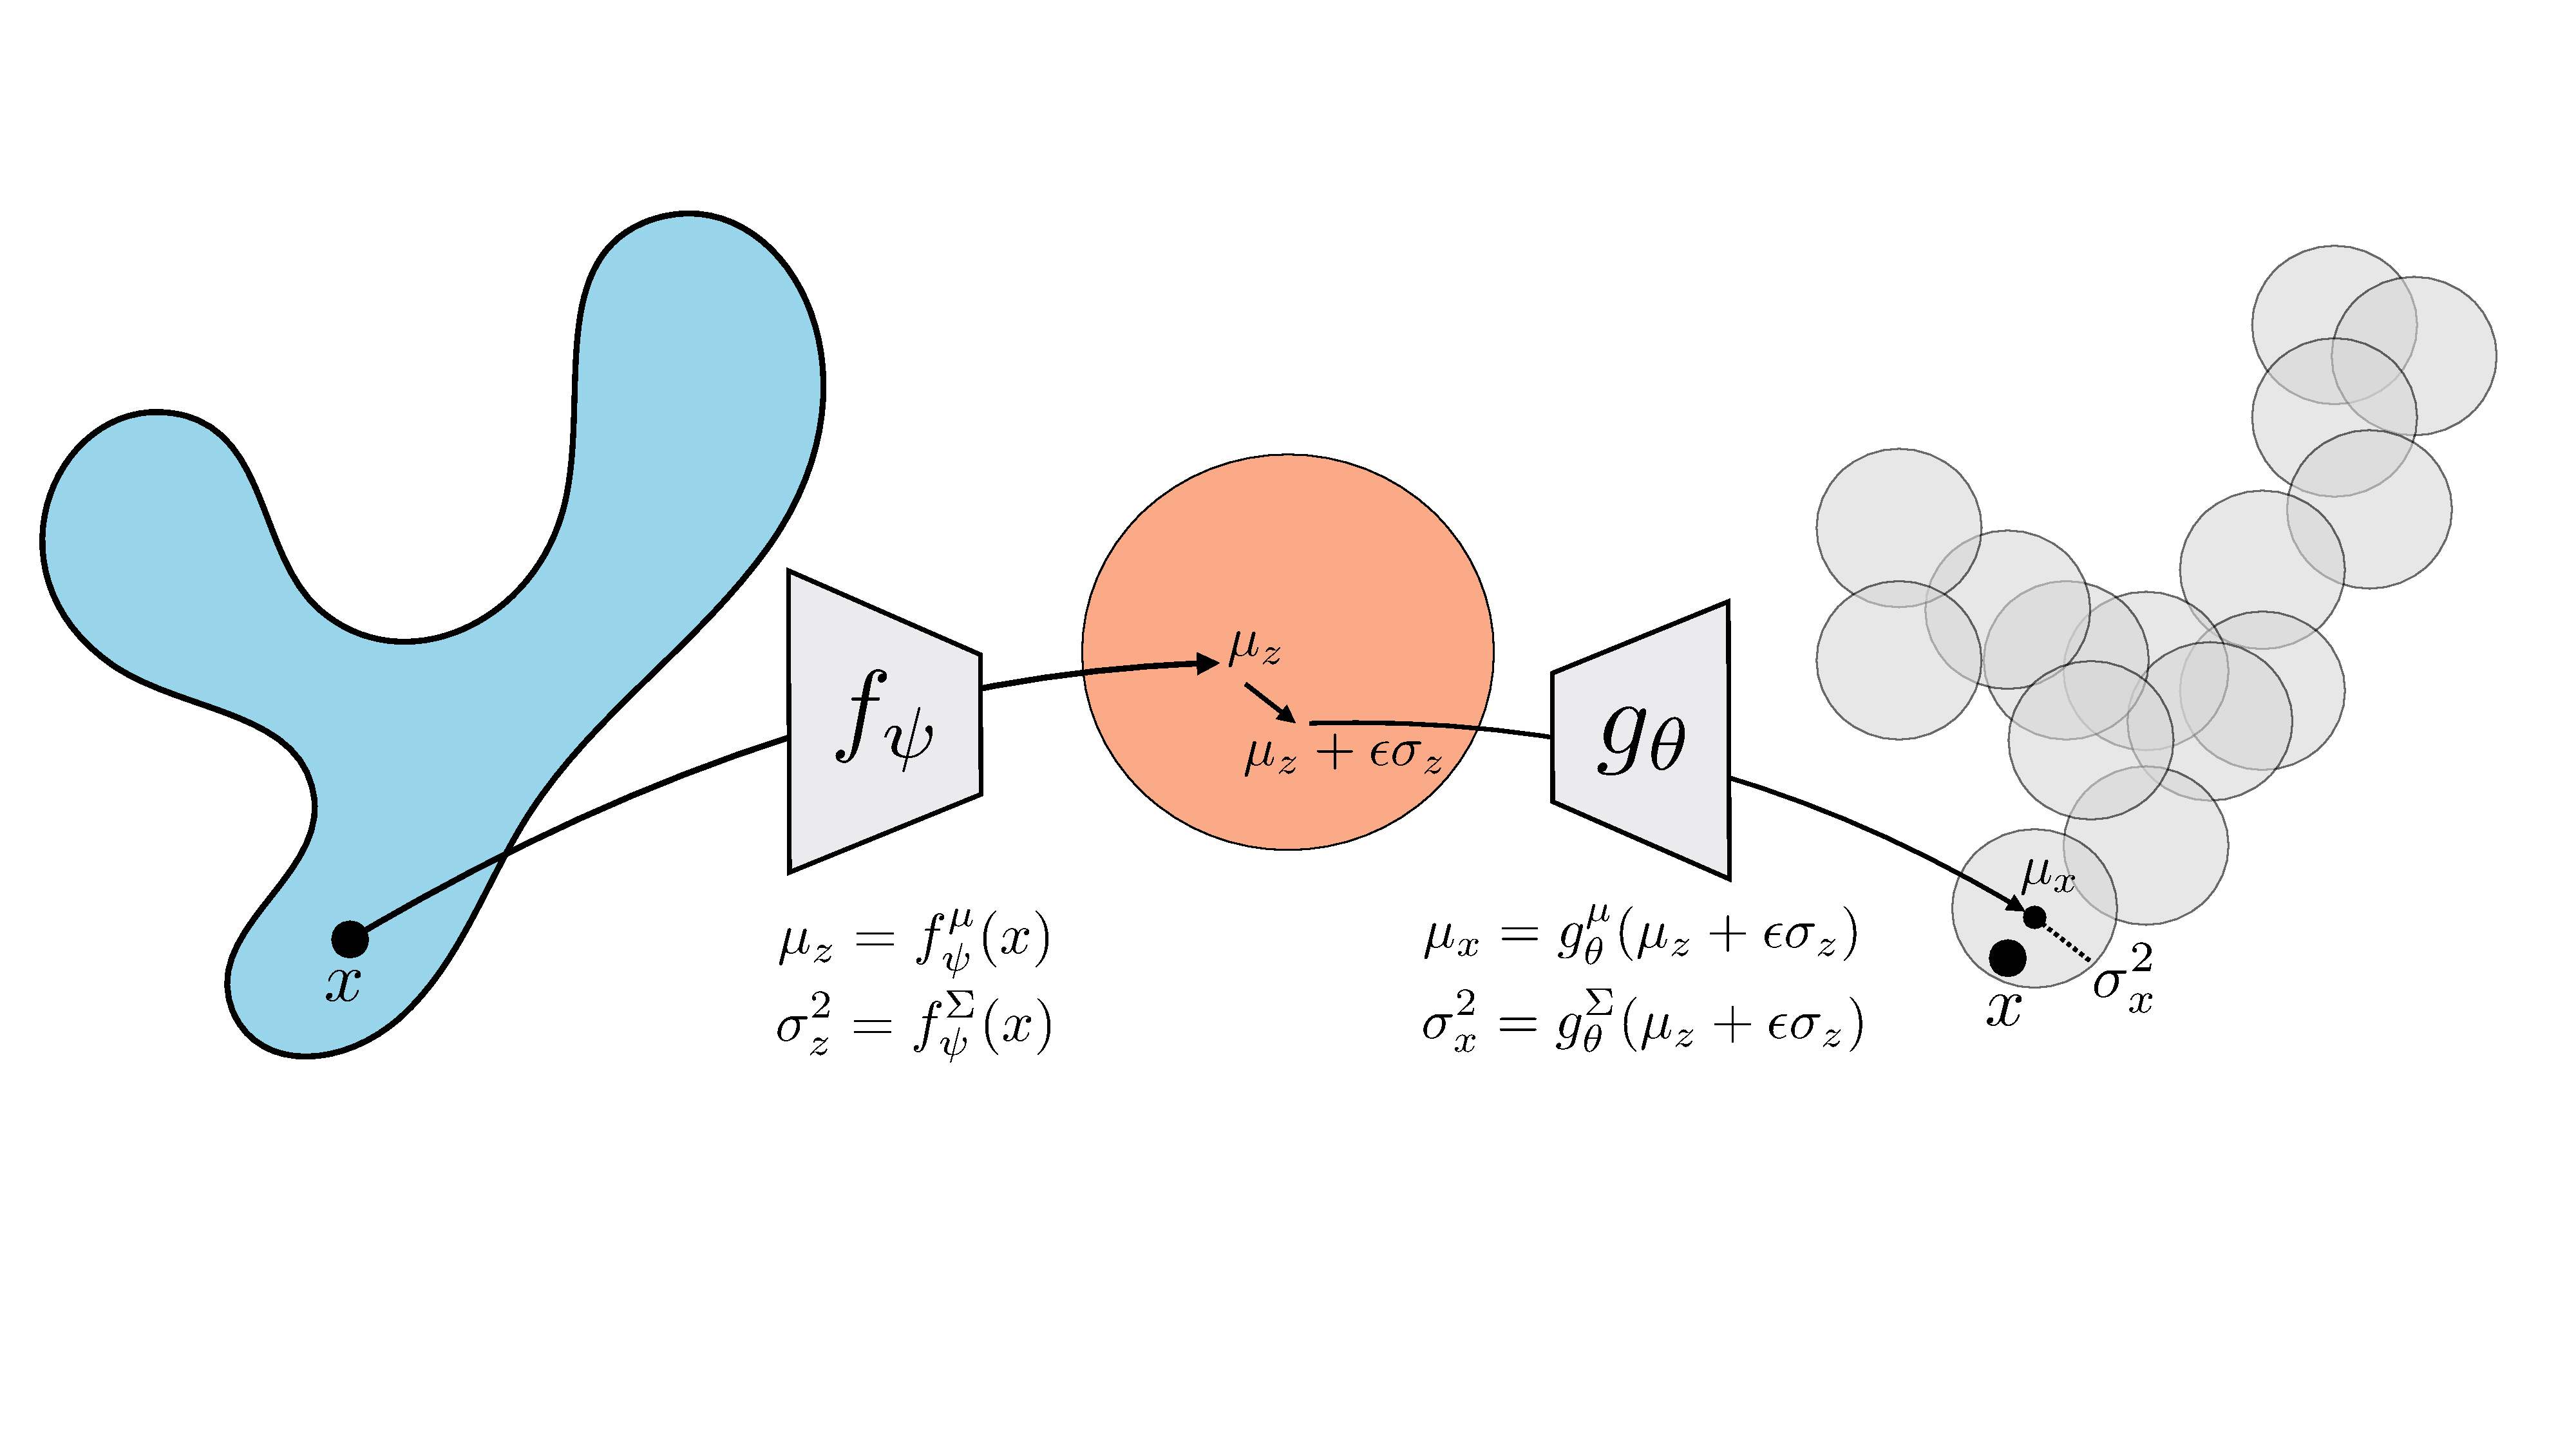
\includegraphics[width=0.8\linewidth]{./figures/generative_modeling_and_representation_learning/VAE_as_autoencoder.pdf}
    }
    \caption{To evaluate the likelihood a VAE places on a datapoint $x$, we encode $x$ into $z$-space and then decode back and compute the reconstruction error. This corresponds to one importance sample for approximating the likelihood function.}
\label{fig:generative_modeling_and_representation_learning:VAE_as_autoencoder}
\end{figure}

The only differences from an autoencoder are that 1) we sample a stochastic $z$ from the output of the encoder, 2) the reconstruction error is scaled and offset by the predicted variance of the Gaussian likelihood model, and 3) we add to this term the KL loss defined previously.

Difference \#1 is worth remarking on. To train the VAE, we need to backpropagate through the sampling step in \eqn{\ref{eqn:generative_modeling_meets_representation_learning:sampling_z_step}}. How can we backpropagate through the sampling operation? The way to do this turns out to be quite simple: we reparameterize sampling from $\mathcal{N}(\mu_z, \sigma^2_z)$ as follows:
\begin{align}
    \epsilon \sim \mathcal{N}(0,1)\\
    z = \mu_z + \epsilon \sigma_z
\end{align}
This step is known as the \index{Reparameterization trick}\textbf{reparameterization trick}, as it reparameterizes a stochastic function (sampling from a Gaussian parameterized by a neural net) to be a deterministic transformation of a fixed noise source (the unit Gaussian). To optimize the parameters for the encoder, we only need to backprogate through $\mu_z$ and $\sigma_z$, which are deterministic functions of $x$, and therefore we have sidestepped the need to handle backpropagation through a stochastic function.%This trick allows us to differentiate through the system we are building up; in particular we can compute $\frac{\partial z}{\partial \psi}$, which we will need in order to know how to update the parameters $\psi$ of the encoder to produce samples $z$ that place higher likelihood on our data.

Putting all the terms together, the objective we are maximizing can now be written as:
\begin{align}
     \frac{1}{N}\sum_{i=1}^N \Big( \log\frac{1}{\sigma_{x^{(i)}}\sqrt{2\pi}} - \frac{\overbrace{(x^{(i)} - \mu_{x^{(i)}})^2}^{\text{reconstruction error}}}{2\sigma_{x^{(i)}}^2} - \underbrace{\frac{1}{2}(\mu_{z^{(i)}}^2 + \sigma_{z^{(i)}}^2 - \log(\sigma_{z^{(i)}}^2) - 1)}_{\text{KL term}} \Big)
\end{align}
\marginnote{$x^{(i)}$ is the $i$-th datapoint in our training set and $z^{(i)}$ is its encoding.}
The KL term encourages the encodings $z^{(i)}$ to be near a unit Gaussian distribution. To get an intuition for the effect of this term, consider the case where we fix $\sigma_{z^{(i)}}$ to be 1; this is still a valid model for $q_{\psi}(Z|x)$, just with lower capacity because it has fewer free parameters. In this simple case, the KL term reduces to $\frac{1}{2}(\mu_{z^{(i)}}^2 - 1) \propto \mu_{z^{(i)}}^2$. The effect of this term is therefore to encourage the encodings $\mu_{z^{(i)}}$ to be \textit{as close to zero as possible}. In other words, the KL term squashes the distribution of latents ($q_{\psi}(Z)$) to be near the origin. Minimizing the reconstruction error, on the other hand, requires that the latents do not collapse to the origin; this term wants them to be as spread out as possible so as to preserve information about the inputs $x^{(i)}$ that they encode. The tension between these two terms is what causes the VAE to work. While a standard autoencoder may produce an arbitrary latent distribution, with gaps and tendrils of density (as we saw in \fig{\ref{fig:generative_modeling_and_representation_learning:autoencoder_complicated_latent_space}}), a VAE produces a tightly packed latent space which can be densely sampled from.


% In this section we will assume the following models for all the important distributions:


% As shorthand, we will use the following notation the output of the encoder and decoder:


% The KL-divergence between two Gaussians has a closed form:

% See XX for a derivation.

% For the other term, we will use importance sampling, as described previously. 

% For a given $\mathbf{x}^{(i)}$, we approximate the expectation via sampling z given x.

% Given a datapoint $x$, we wish to compute the probability of that datapoint under our model, $p_{\theta}(x)$. As discussed previously, this can be estimated by importance sampling where we measure $p_{\theta}(x | z)$ by sampling from the distribution $q_{\psi}(Z \given x)$:
% \begin{align}
% p_{\theta}(x) &= \mathbb{E}_{z\sim q_{\psi}(Z \given x)}\Big[\frac{p_{z}(z)}{q_{\psi}(z \given x)} p_{\theta}(x \given z)\Big]\label{eqn:generative_modeling_and_representation_learning:p_x_connection_to_autoencoders}
% \end{align}
% The way we will model $q_{\psi}(Z \given x)$ is as a Gaussian whose mean and variance are the output of an encoder $f_{\psi}$ applied to $x$:
% \begin{align}
%      \mu_z &= f^{\mu}_{\psi}(x), & \sigma_z &= f^{\Sigma}_{\psi}(x)
% \end{align}
% To draw one importance sample, we take a sample from this Gaussian:
% \begin{align}
%     z^\prime \sim \mathcal{N}(\mu_z, \sigma_z)
% \end{align}
% To draw this sample, we will reparameterize $z$ to be a transformation of a unit Gaussian sample:
% \begin{align}
%     \epsilon \sim \mathcal{N}(0,1)\\
%     z^\prime = \mu_z + \epsilon \sigma_z
% \end{align}
% This step is known as the \textbf{reparameterization trick} as it reparameterizes a stochastic function (sampling from a Gaussian parameterized by a neural net) to be a deterministic transformation of a fixed noise source (the unit Gaussian). This trick allows us to differentiate through the system we are building up; in particular we can compute $\frac{\partial z}{\partial \psi}$, which we will need in order to know how to update the parameters $\psi$ of the encoder to produce samples $z$ that place higher likelihood on our data.

% Now that we have our sample $z^\prime$, we use it to evaluate the expectation in \eqn{\ref{eqn:generative_modeling_and_representation_learning:p_x_connection_to_autoencoders}}:
% \begin{align}
%     p_{\theta}(x) \approx \frac{p_{z}(z^\prime)}{q_{\psi}(z^\prime \given x)}p_{\theta}(x \given z^\prime)
% \end{align}


% \begin{figure}[h!]
%     \centerline{
%     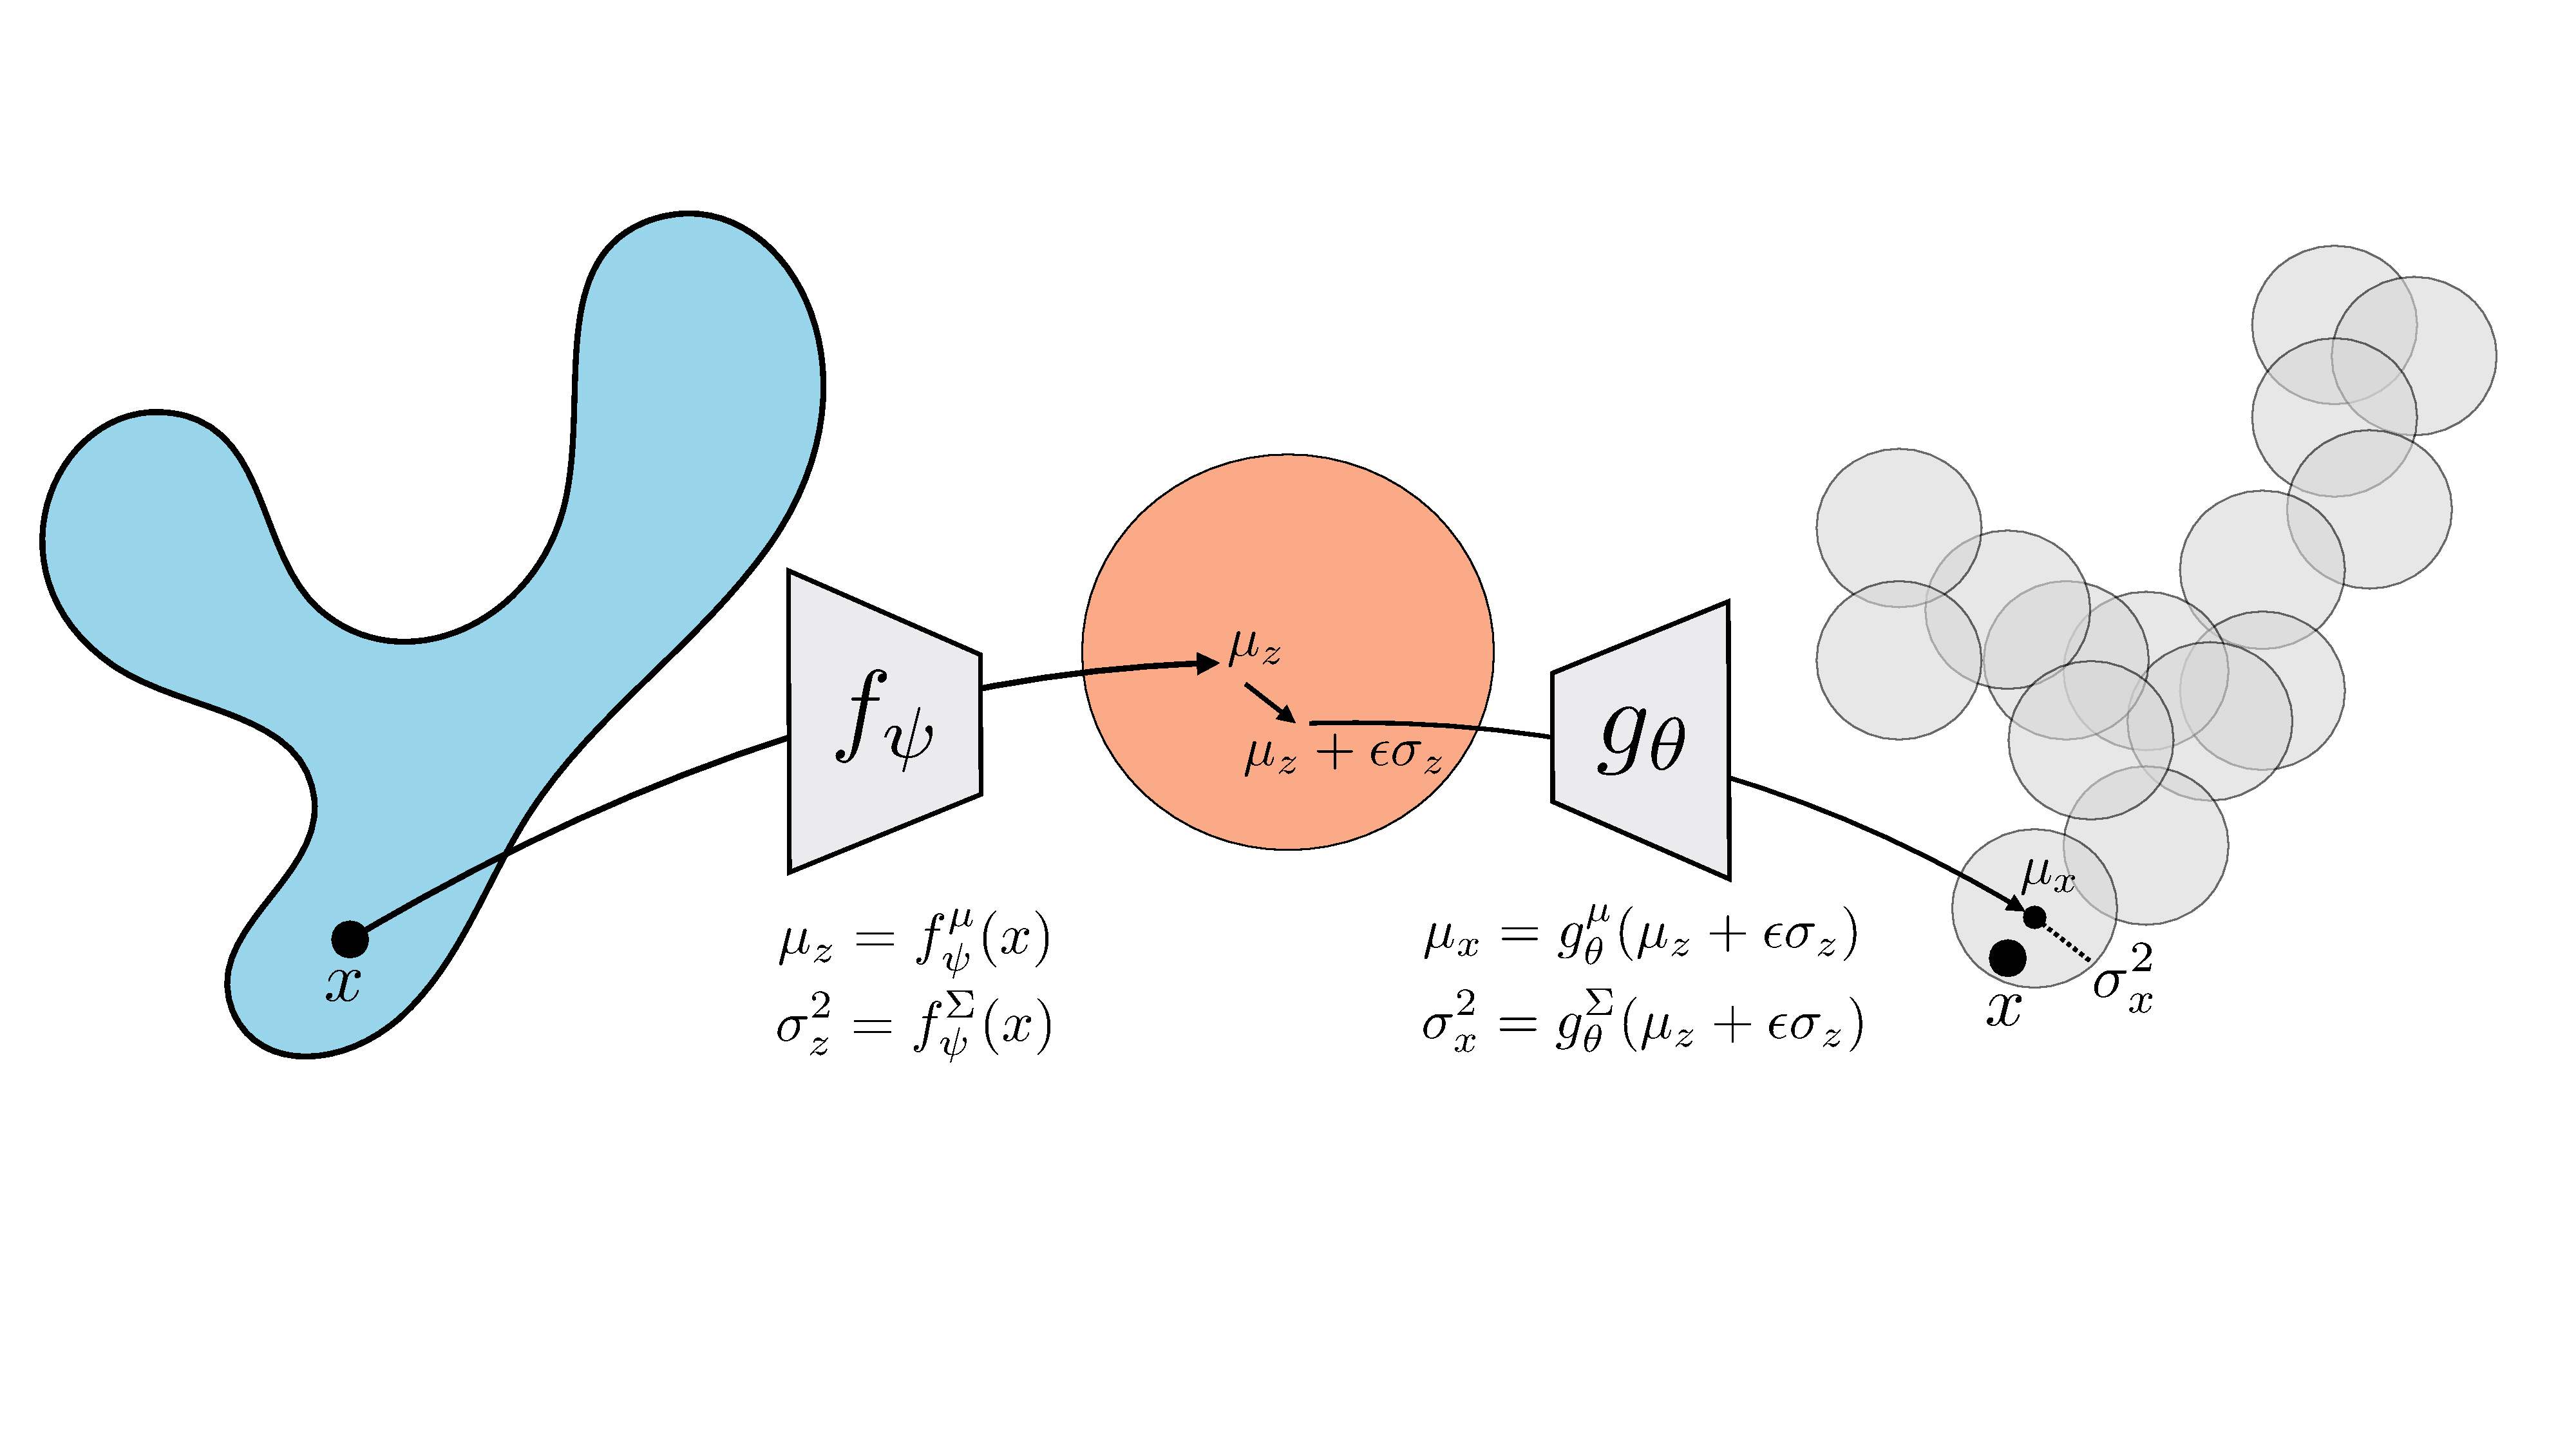
\includegraphics[width=0.8\linewidth]{./figures/generative_modeling_and_representation_learning/VAE_as_autoencoder.pdf}
%     }
%     \caption{To evaluate the likelihood a VAE places on a datapoint $\mathbf{x}$, we encode $\mathbf{x}$ into $z$-space and then decode back and compute the reconstruction error. This corresponds to one importance sample for approximating the likelihood function.}
%     \label{fig:generative_modeling_and_representation_learning:VAE_training_iters}
% \end{figure}

% This allows rewriting the expectation as:
% \begin{align}
%     J &= \mathbb{E}_{\epsilon \sim \mathcal{N}(0,1)}\Big[ - \log \mathcal{N}(x; g^{\mu}_{\theta}(z), g^{\sigma}_{\theta}(z)) \Big] - \KLdiv{q_{\psi}(Z \given x)}{\mathcal{N}(0,1)}\\
%     &= \mathbb{E}_{\epsilon \sim \mathcal{N}(0,1)}\Big[ - \log \mathcal{N}(x; g^{\mu}_{\theta}(f^{\mu}_{\psi}(x) + \epsilon f^{\sigma}_{\psi}(x)), g^{\sigma}_{\theta}(f^{\mu}_{\psi}(x) + \epsilon f^{\sigma}_{\psi}(x))) \Big] \nonumber \\ &\quad\quad - \KLdiv{q_{\psi}(Z \given \mathbf{x})}{\mathcal{N}(0,1)}\\
%     &= \mathbb{E}_{\epsilon \sim \mathcal{N}(0,1)}\Big[ \log\frac{1}{\sigma\sqrt{2\pi}} - \frac{\overbrace{(x - \mu)^2}^{\text{reconstruction error}}}{2\sigma^2} \Big] - \KLdiv{q_{\psi}(Z \given \mathbf{x})}{\mathcal{N}(0,1)}\\
%     & \quad\quad \mu = \underbrace{g^{\mu}_{\theta}(f^{\mu}_{\psi}(x) + \epsilon f^{\sigma}_{\psi}(x))}_{\text{noisy autoencoder}}, \quad\quad \sigma = g^{\sigma}_{\theta}(f^{\mu}_{\psi}(x) + \epsilon f^{\sigma}_{\psi}(x))) \nonumber
% \end{align}
% What this shows is that to compute the VAE's objective, you simply run an autoencoder with noise added to the bottleneck, as shown in \fig{\ref{}}:

% The cost function is then the reconstruction error (same as with regular autoencoders) weighted by a term related to the variance of the noise added and also with an additional KL divergence term to squish the latent distribution toward the unit Gaussian.

% To train a VAE we normally are not just fitting a single $\mathbf{x}$ but maximizing the likelihood of a dataset $\{\mathbf{x}^{(i)}\}_{i=1}^N$, so the cost we optimize is $\sum_i J(\mathbf{x}^{(i)}, \theta, \phi)$. Optimization of VAE proceeds as follows:
% \begin{itemize}
%     \item Sample one or more $\mathbf{x} \sim \{\mathbf{x}^{(i)}\}_{i=1}^N$.
%     \item \textit{Encode} the data with a forward pass through $f_{\psi}$.
%     \item For each datapoint, create one or more noisy latent codes using the distribution parameterized by the encoder.
%     \item \textit{Decode} the data by passing the noisy latent codes through the $g_{\theta}$.
%     \item Compute the losses and backprop to update $\theta$ and $\psi$.
% \end{itemize}
% In most implementations of VAEs, only a single sample from the latent distribution is used for each datapoint on each iteration of backpropagation.%\marginnote{VAE's are usually presented as maximizing a lower-bound (the ELBO: $-J$). But, when only a single latent sample is used to compute the gradient update, then there is no difference between the form of the gradient update for the lower-bound objective $-J$ and the update for the exact objective $-J_p$. If you prefer to consider VAE's as approximately maximizing data likelihood, rather than approximately maximizing a lower-bound on data likelihood, then that is perfectly consistent with practical implementations (but deviates from the formalisms in most literature on the subject).}[-0.4cm]

These effects can be seen in \fig{\ref{fig:generative_modeling_and_representation_learning:VAE_training_iters}}, where we show three checkpoints of optimizing a VAE. As in the infinite mixture of Gaussians example shown previously, we again assume an isotropic Gaussian model for the decoder, and here also assume that model for the encoder.
\begin{figure}[h!]
    \centerline{
    \includegraphics[width=1.0\linewidth]{./figures/generative_modeling_and_representation_learning/VAE_training_iters.pdf}
    }
    \caption{Training a VAE to model the blue distribution. The Gaussian components spread out to tile both the embedding space and the data space.}
    \label{fig:generative_modeling_and_representation_learning:VAE_training_iters}
\end{figure}


%We can alternate between updating p, then updating q. They help each other.

%We can simplify things a bit by noticing that the objective for q is a lower-bound on the objective for p. If we optimize it w.r.t. p then we are optimizing a lower-bound on likelihood and that still ends up maximizing likelihood. This is in fact how VAE's are defined, but note that you could instead optimize p with the exact objective and that would be a sound strategy that leads to the same answer.




%Remember, the only distributions for which we have so far defined simple forms are $p_{\theta}(\mathbf{x} | \mathbf{z})$ and $p_{\mathbf{z}}(\mathbf{z})$, which are both Gaussians. By Bayes' rule, we can write $p_{\theta}(\mathbf{z} | \mathbf{x})$ in terms of these distributions:
%\begin{align}
%    p_{\theta}(\mathbf{z} | \mathbf{x}) = \frac{p_{\theta}(\mathbf{x} | \mathbf{z})p_{\mathbf{z}}(\mathbf{z})}{\int_{\mathbf{z}} p_{\theta}(\mathbf{x} | \mathbf{z})p_{\mathbf{z}}(\mathbf{z})d\mathbf{z}}
%\end{align}
%Computing $p_{\theta}(\mathbf{z} | \mathbf{x})$ requires evaluating another intractable integral over $\mathbf{z}$!


%It's intractable -- another integral. What we will do is instead use a surrogate density q in a tractable family, i.e. one for which $q(\mathbf{z} | \mathbf{x})$ can be efficiently evaluated. What we will do is try to find a function $q_{\psi}$, within a parameterized family of densities, that is as close as possible to the optimal sampling density $p_{\theta}(\mathbf{z}|\mathbf{x})$.\marginnote{This idea is called \textbf{variational inference}: to model an intractable density $p$, use the nearest density in a tractable family $q$. This is where the V comes from in the VAE's name.} We will use $\texttt{KL}$-divergence to measure closeness and search for the $q_{\psi}(\mathbf{z}|\mathbf{x})$ that minimizes the $\texttt{KL}$-divergence from $p_{\theta}(\mathbf{z}|\mathbf{x})$:




% Alas, evaluating this KL-divergence requires evaluating $p_{\theta}(\mathbf{z}|\mathbf{x})$, which yields another intractable integral. Fortunately, something rather magical happens when we do a few algebraic manipulations:
% \begin{align}
%     \texttt{KL}(q_{\phi}(\mathbf{z}|\mathbf{x}), p_{\theta}(\mathbf{z}|\mathbf{x})) &= \mathbb{E}_{q_{\phi}(\mathbf{z}|\mathbf{x})}[\log q_{\phi}(\mathbf{z}|\mathbf{x}) - \log p_{\theta}(\mathbf{z}|\mathbf{x})]\\
%     &= \mathbb{E}_{q_{\phi}(\mathbf{z}|\mathbf{x})}[\log q_{\phi}(\mathbf{z}|\mathbf{x}) - \log p_{\theta}(\mathbf{z}, \mathbf{x})] + \log p_{\theta}(\mathbf{x})\\
%     &= -\mathcal{L}(\mathbf{x}, \theta, \phi) + \log p_{\theta}(\mathbf{x})\\
%     &= -\mathcal{L}(\mathbf{x}, \theta, \phi) + \log L(\mathbf{x}, \theta)\\
%     \mathcal{L}(\mathbf{x}, \theta, \phi) &= \log p_{\theta}(\mathbf(x)) - \texttt{KL}(q_{\phi}(\mathbf{z}|\mathbf{x}), p_{\theta}(\mathbf{z}|\mathbf{x}))\\
%     &\leq \log p_{\theta}(\mathbf(x))
% \end{align}

% Now $\mathcal{L}$ is something we can actually evaluate and therefore optimize over! Notice that $\mathcal{L}$ is a lower-bound on the log likelihood of the data (last line, because KL-divergence is always non-negative), and because of this $\mathcal{L}$ is referred to as the {\bf Evidence Lower-Bound} or {\bf ELBO}. Because $\mathcal{L}$ is a lower-bound, gradient ascent on $\mathcal{L}$, w.r.t. parameters $\theta$ and $\phi$ will produce a model $p_{\theta}$ that places maximum likelihood on the data. Interestingly, as $\mathcal{L}$ is being maximized, the gap between the $\mathcal{L}$ and $\log L$ will eventually have to decrease, as we approach the true max likelihood model in the family of functions we are optimizing over. That means that $\texttt{KL}(q_{\phi}(\mathbf{z}|\mathbf{x}), p_{\theta}(\mathbf{z}|\mathbf{x}))$ will have to decrease, since it equals the gap between $\mathcal{L}$ and $\log L$. Therefore something really neat has happened, we are getting better and better importance weights $q$ as the model $p$ also gets better and better, and the better the importance weights are, the better, in turn, is our ability to estimate likelihood from just a few samples. It turns out that in practice, one sample per $\mathbf{x}$ per step of gradient ascent is enough, because over the course of optimization this single sample becomes a better and better estimate of the likelihood we are trying to optimize.

% A longer treatment on VAEs is given in \cite{doersch2016tutorial}.



\section{Do VAEs Learn Good Representations?}

One perspective on VAEs is that they are a way to train a generative model $p_{\theta}$. From this perspective, the encoder is just scaffolding for learning a decoder. However, the encoder can also be useful as an end in itself, and we might instead think of the decoder as scaffolding for training an encoder. This was the perspective presented by autoencoders, after all, and the VAE encoder comes with the same useful properties: it maps data to a low-dimensional latent code that preserves information about the input. In fact, from a representation learning perspective, VAEs even go beyond autoencoders. Not only do VAEs learn a compressed embedding, the embeddings may also have other desirable properties depending on the prior $p_{\mathbf{z}}$. For example, if $p_{\mathbf{z}} = \mathcal{N}(0,1)$, as is common, then the loss encourages that the dimensions of the embedding are independent, a property called \index{Disentangled representation}\textbf{disentanglement}.%, 2) the embeddings are uniformly distributed near the surface of the unit hypersphere (this is a property of high-dimensional Gaussians).

Disentanglement means that we can vary one dimension of the embedding at time, and just one independent factor of variation in the generated images will change. For example, one dimension might control the direction of light in a scene and another dimension might control the intensity of light.

\subsection{Example: Learning a VAE for Rivers}
Suppose we have a dataset of aerial views of rivers. We wish to fit this data with a VAE so that (1) we can generate new rivers, and (2) we can identify the underlying latent variables that explain river appearance. In this example we will use data for which we know the true data generating process, which is simply a Python script that procedurally synthesizes cartoon images of rivers given input noise (this is a more elaborate version of the script we saw in \algref{\ref{alg:generative_models:simple_rivers_script}} of \chap{\ref{chapter:generative_models}
}). The script takes in random values that control the attributes of the scene (the grass color, the heading of the river, the number of trees, etc.) and generates an image with these attributes, as shown in \fig{\ref{fig:generative_modeling_and_representation_learning:rivers_dataset}}.
\begin{figure}[h!]
    \centerline{
    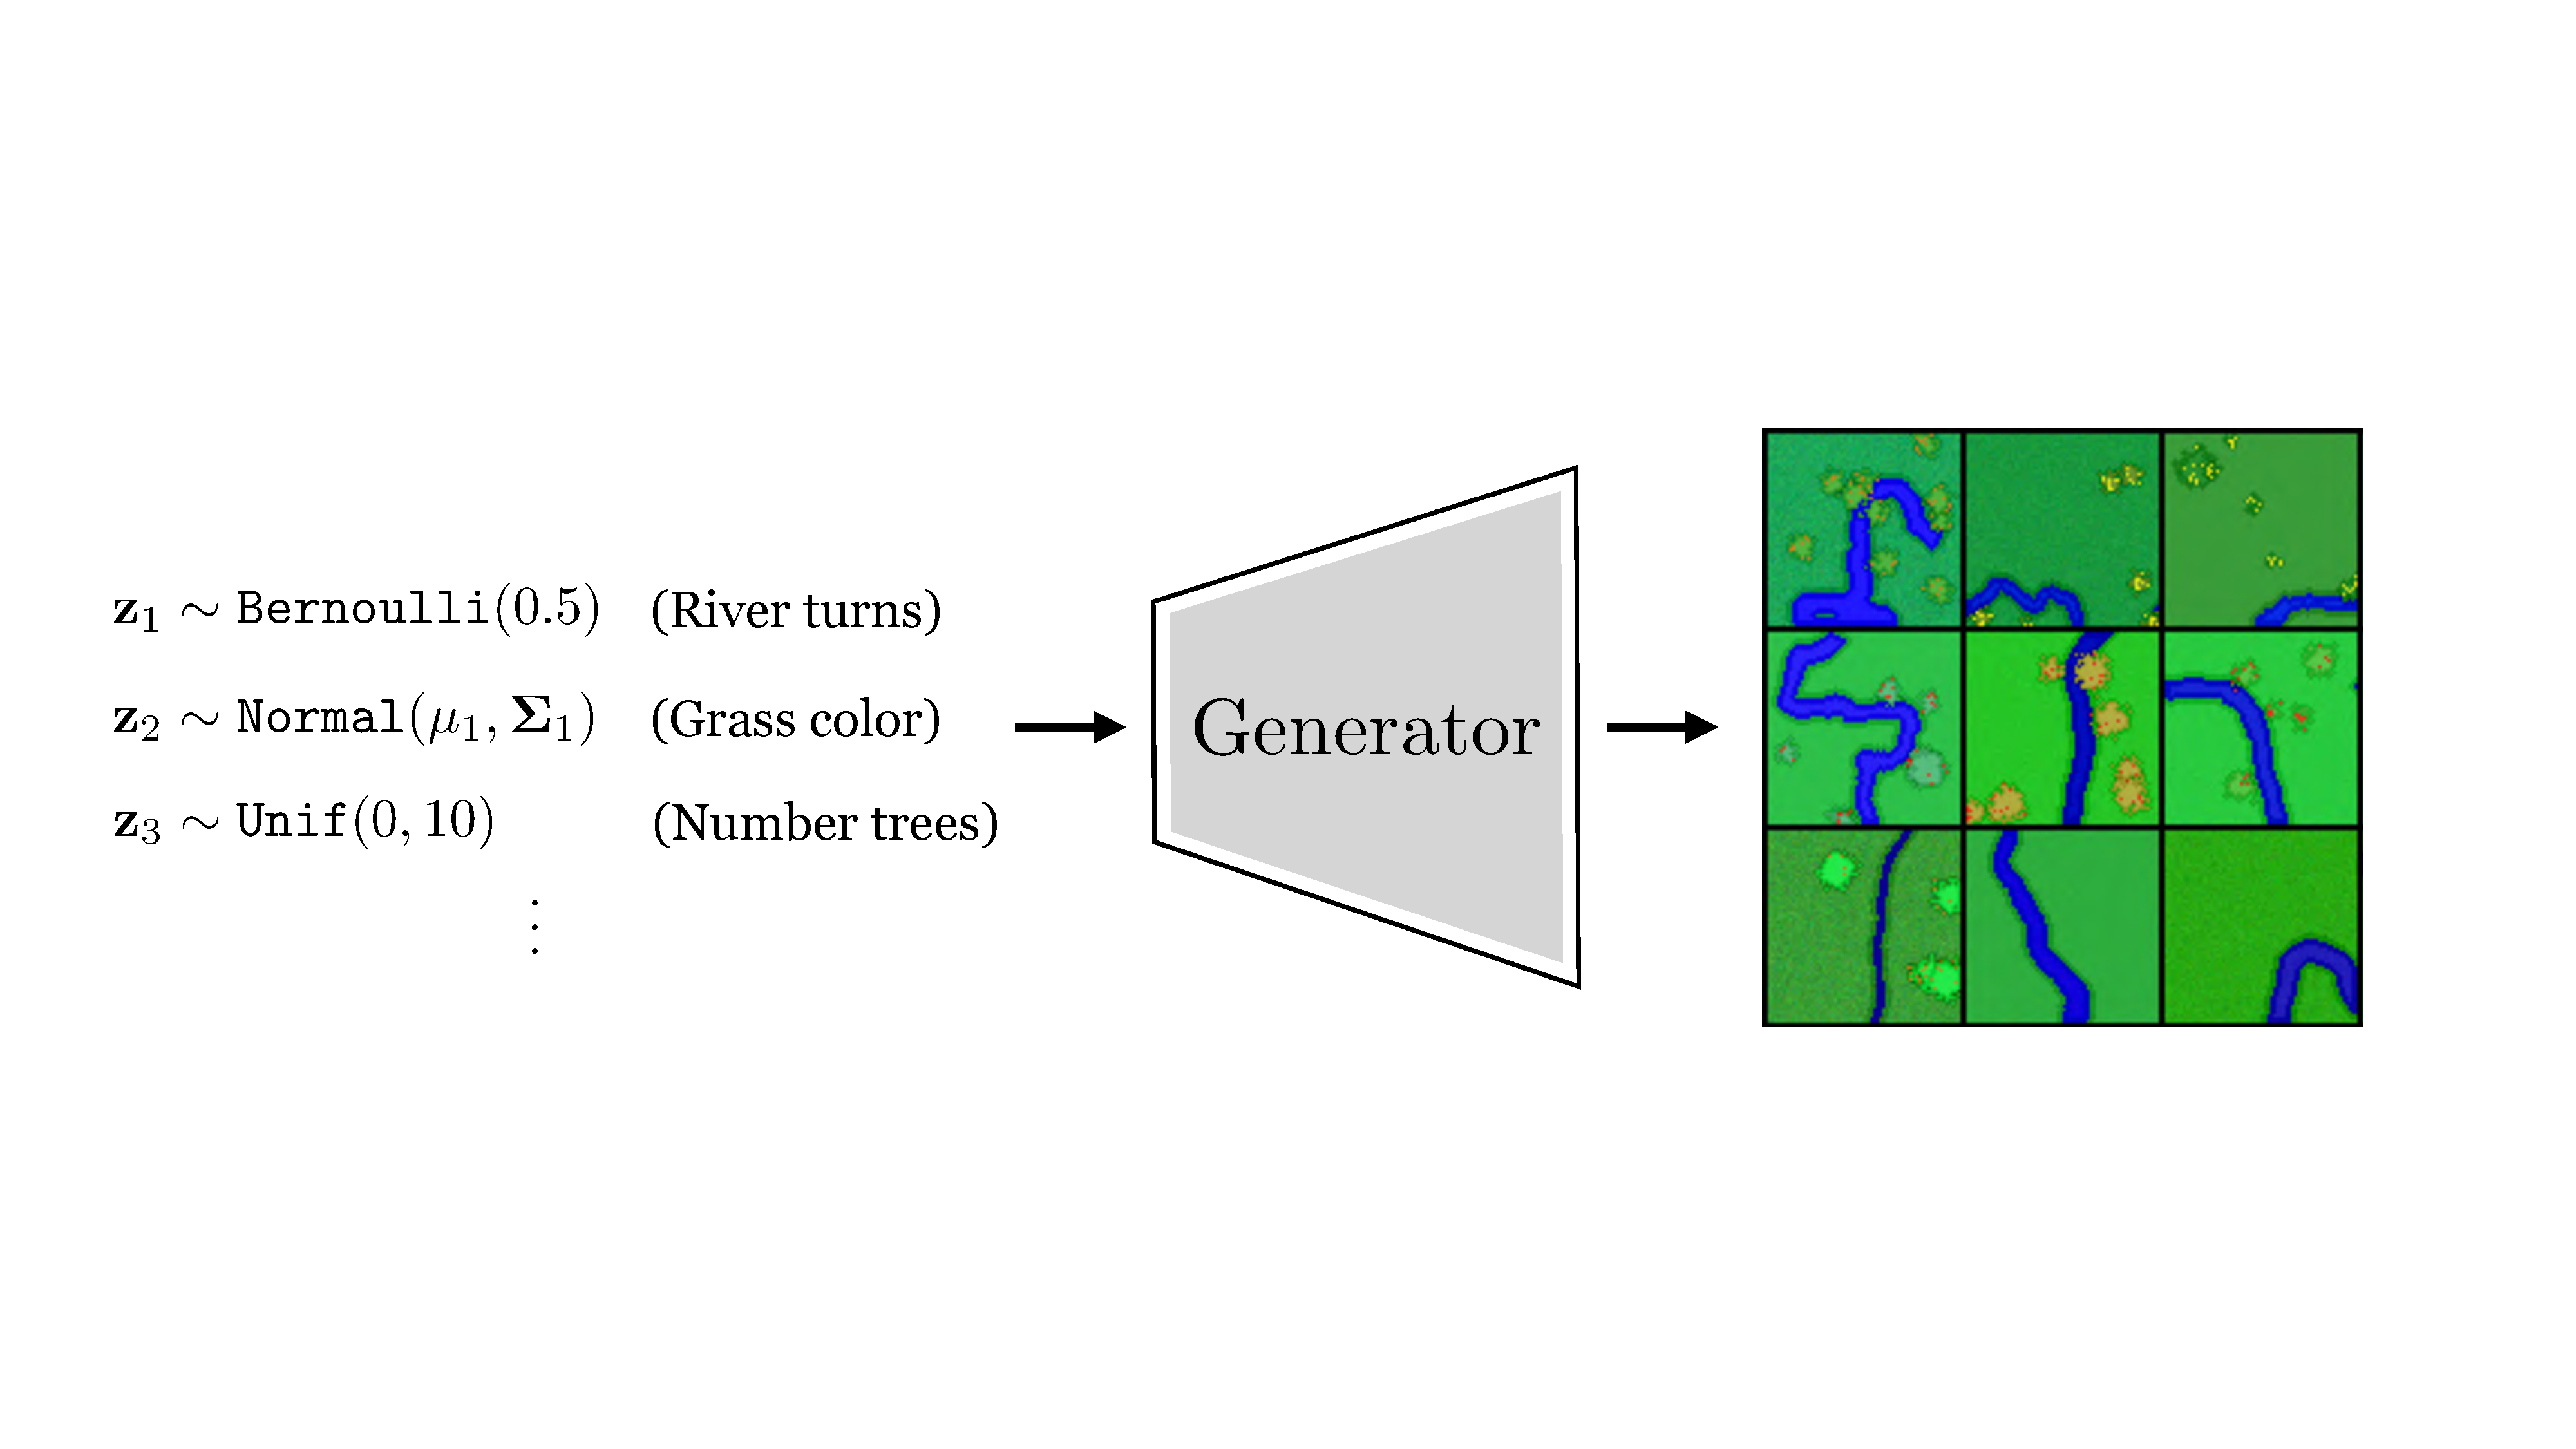
\includegraphics[width=0.8\linewidth]{./figures/generative_modeling_and_representation_learning/rivers_dataset.pdf}
    }
    \caption{A toy generative model hand-coded in Python.}
    \label{fig:generative_modeling_and_representation_learning:rivers_dataset}
\end{figure}

Training a VAE on this data (\fig{\ref{fig:generative_modeling_and_representation_learning:vae_rivers_samples}}) learns to recreate the generative process with a \textit{neural net} (rather than a Python script) and maps zero-mean unit-variance \textit{Gaussian noise} to images (rather than taking as input the noise types the script uses).
\begin{figure}[h!]
    \centerline{
    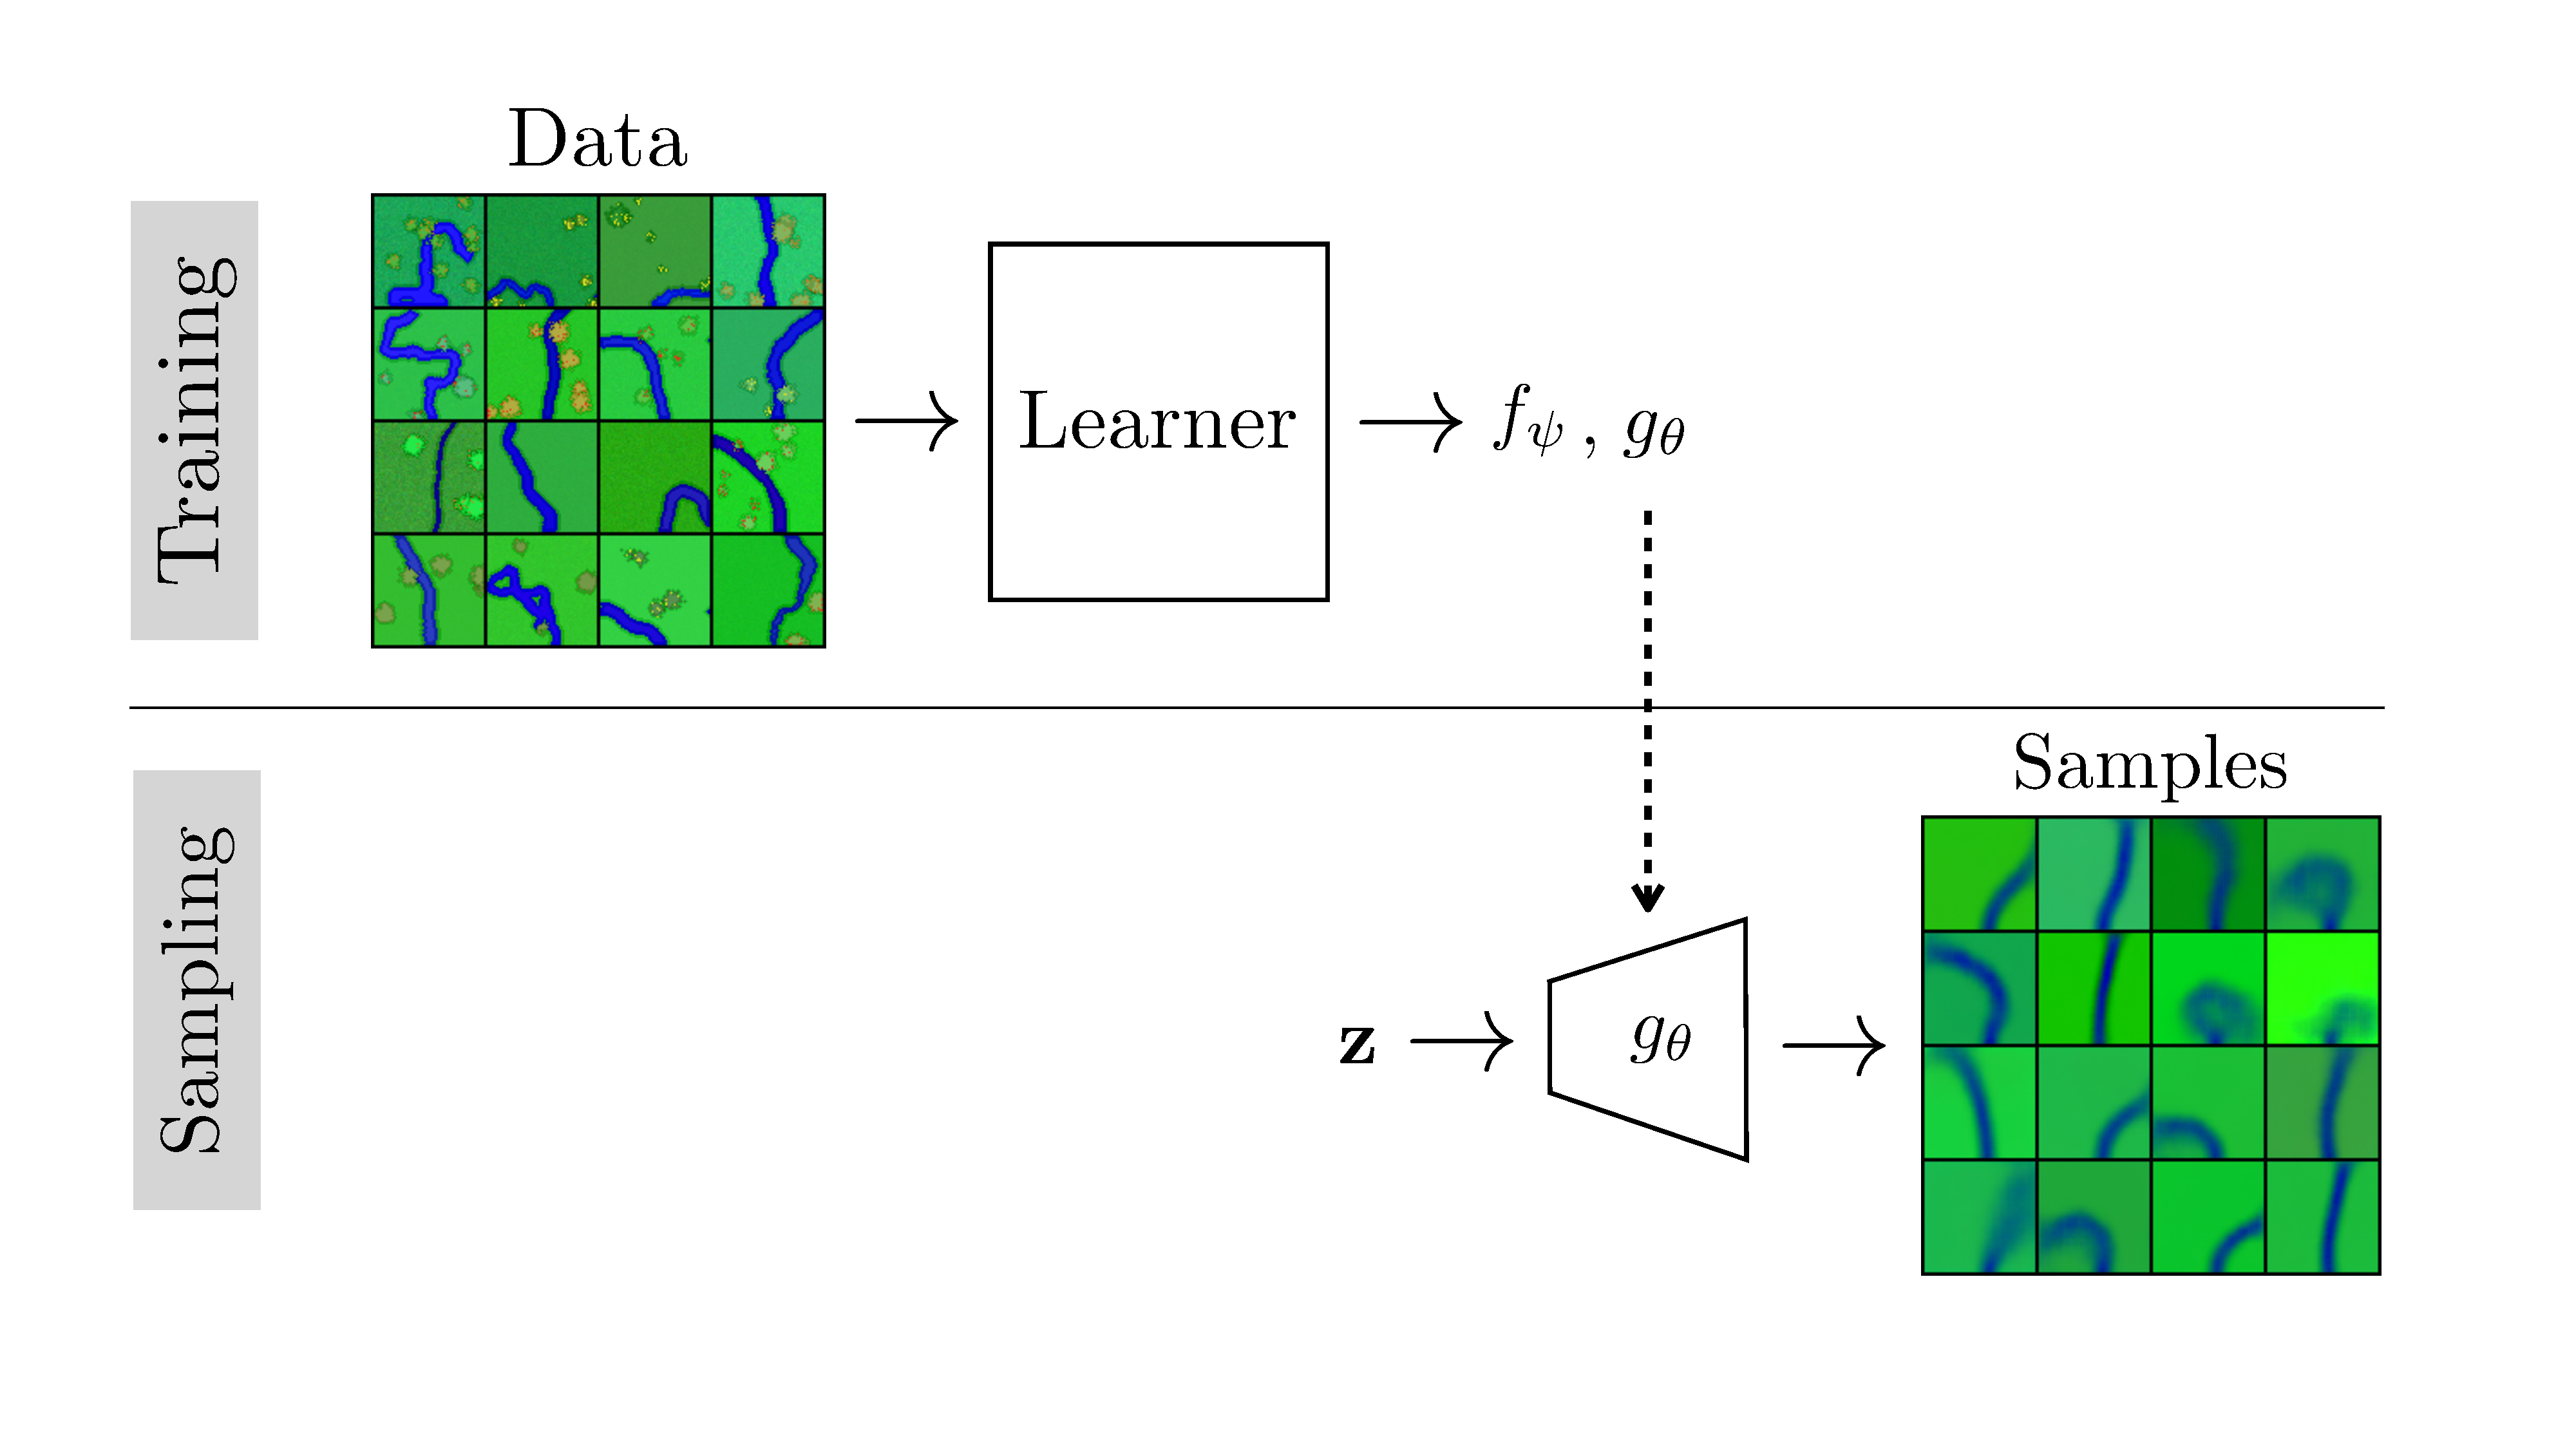
\includegraphics[width=1.0\linewidth]{./figures/generative_modeling_and_representation_learning/vae_rivers_samples.pdf}
    }
    \caption{Fitting a VAE to the rivers dataset}
    \label{fig:generative_modeling_and_representation_learning:vae_rivers_samples}
\end{figure}

Did the VAE uncover the \textit{true} latent variables that generated the data, that is, did it recover latent dimensions corresponding to the attribute values that were the inputs to the Python script? We can examine this by generating a set of images that walk along two latent dimensions of the VAE's $z$-space, shown in \fig{\ref{fig:generative_modeling_and_representation_learning:vae_rivers_latent_walk}}.
\begin{figure}[h!]
    \centerline{
    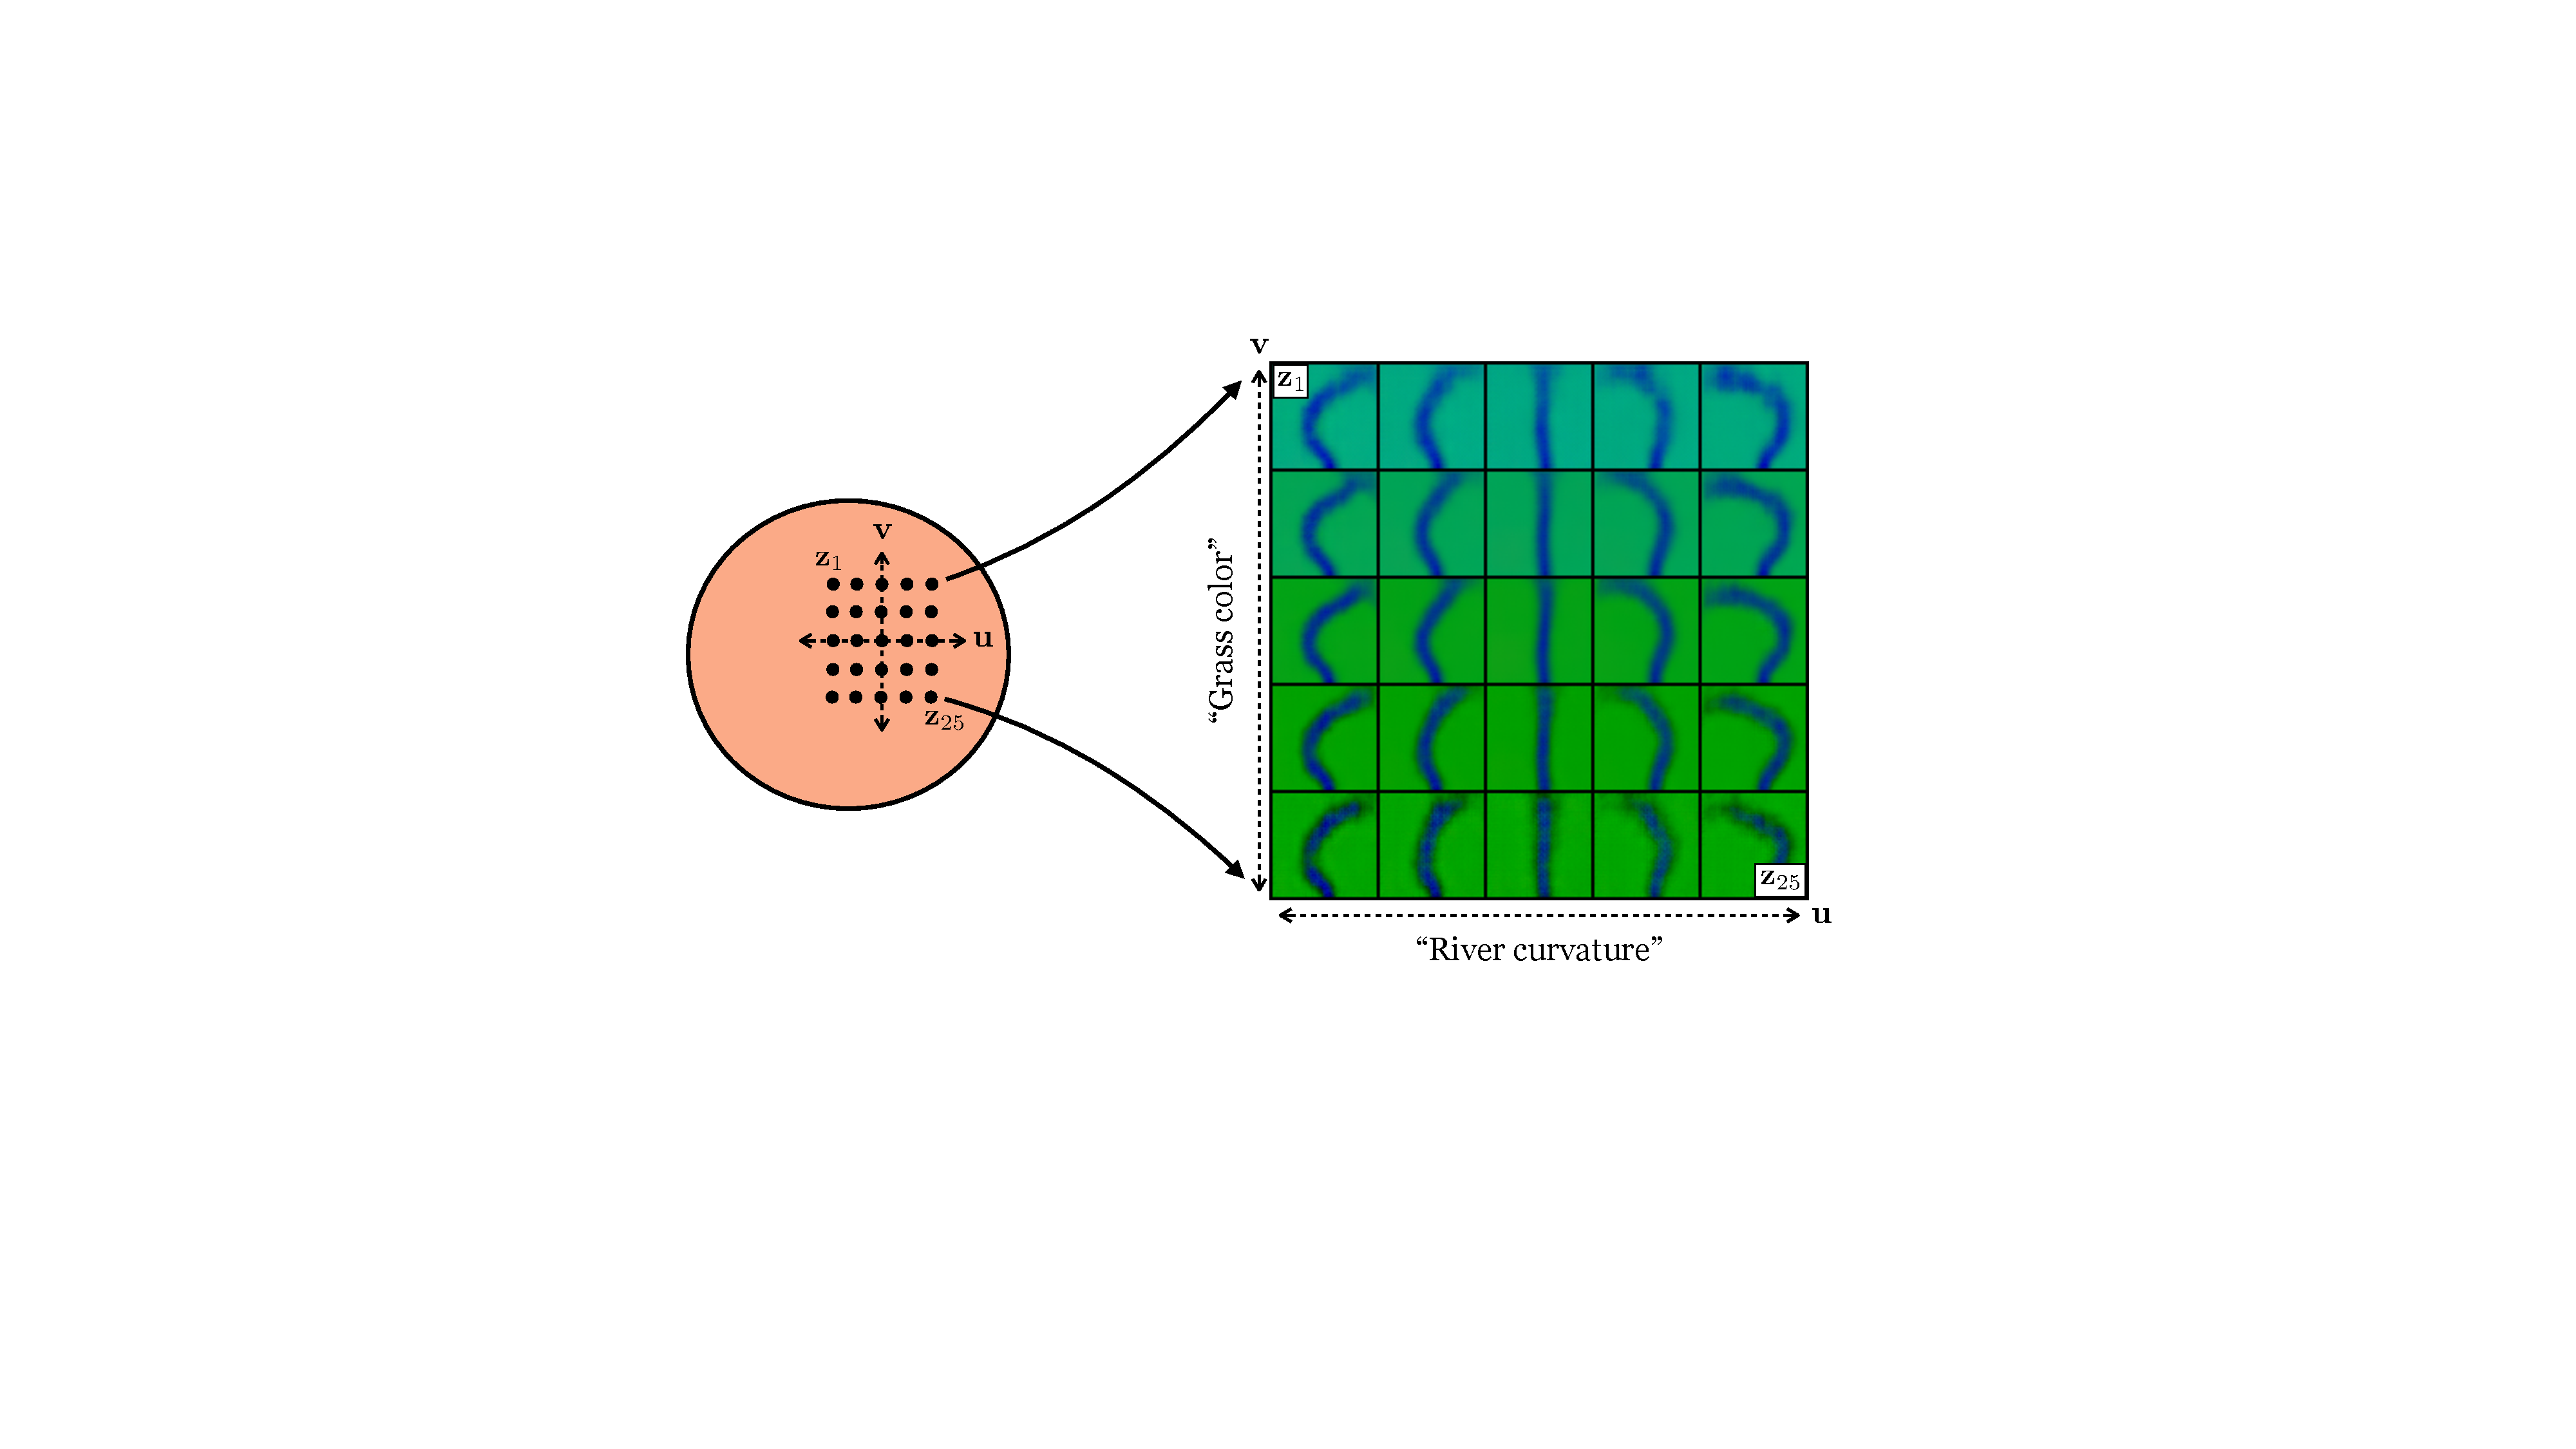
\includegraphics[width=0.75\linewidth]{./figures/generative_modeling_and_representation_learning/vae_rivers_latent_walk.pdf}
    }
    \caption{Walking along two axes of latent space generates images that show variation in two distinct attributes, demonstrating that this model is, to a degree, disentangled.}
    \label{fig:generative_modeling_and_representation_learning:vae_rivers_latent_walk}
\end{figure}

One of the latent dimensions seems to control the grass color, and another controls the river curvature! These two latent dimensions are disentangled in the sense that varying the latent dimension that controls color has little effect on curvature and varying the latent dimension that controls curvature has little effect on color. Indeed, grass color was one of the attributes of the true data generating process (the Python script), and the VAE recovered it. However, interestingly there was no single input to the script that controls the overall river curvature, instead the curves are generating by a vector of Bernoulli variables that rotate the heading left and right as the river extends (using the same algorithm as in \algref{\ref{alg:generative_models:simple_rivers_script}} of \chap{\ref{chapter:generative_models}}). The VAE has discovered a latent dimension that somehow summarizes a more global mode of behavior (i.e., bend left or bend right) than is explicit in the Python script. It is important to realize that VAEs, and most representation learning methods, do not necessarily recover the true causal mechanisms that generated the data but rather might find other mechanisms that can equivalently explain the data.\marginnote{A formal name for this issue is the \index{Nonidentifiability}\textbf{nonidentifiability} of the true parameters that generated a dataset.}[-0.2cm]

% \\
To summarize this section, we have seen that a VAE can be considered two things:
\begin{itemize}
    \item An efficient way to optimize an infinite mixture of Gaussians generative model.
    \item A way to learn a low-dimensional, disentangled representation that can reconstruct the data.
\end{itemize}



%\section{Generative adversarial networks}

%That means wiggling parameters to increase $\mathcal{L}$ will \textit{have to} 

%How should we measure the distance between $q_{\phi}$ and $p_{\theta}(\mathbf{z}|\mathbf{x})$? We will use the KL-divergence between the two distributions, i.e. $\texttt{KL}(q_{\phi}(\mathbf{z}|\mathbf{x}), p_{\theta}(\mathbf{z}|\mathbf{x}))$. Now we have two goals: 1) minimize this KL-divergence to get a good $q_{\phi}$ for importance sampling, and 2) maximize the data likelihood, using importance sampling to efficiently estimate it.

% In VAEs, rather than directly maximizing the likelihood function in Eqn. \ref{eqn:generative_models:vae_likelihood2}, we instead take the $\log$ of the term inside the expectation:
% \begin{align}
%     \mathcal{L}(\mathbf{x}, \theta) &= \mathbb{E}_{\mathbf{z}\sim p(\mathbf{z})}\Big[ \log p_{\theta}(\mathbf{x} | \mathbf{z})\Big]
% \end{align}
% By Jensen's inequality, this is a lower-bound on the data log likelihood ($\mathbb{E}[\log x] \leq \log \mathbb{E}[x]$). Hence under this transformation, we are maximizing a lower-bound on the data log likelihood. Now we can state the full VAE learning objective:
% \begin{align}
%     \argmin_{\theta,\phi} \texttt{KL}(q_{\phi}(\mathbf{z}|\mathbf{x}), p_{\theta}(\mathbf{z}|\mathbf{x})) + \mathcal{L}(\mathbf{x}, \theta)
% \end{align}

%The next question is then how to choose the best $q$ such that we can get a good approximation to the expectation with just a few samples?

%Here we can use the idea alluded to above, and try to sample $\mathbf{z}$'s such that $p_{\theta}(\mathbf{x} | \mathbf{z})$ is large. 

%We can set this up as an optimization problem. First, notice that:
%\begin{align}
%     \frac{1}{N} \sum_{i=1}^N \frac{p(\mathbf{z}_i)}{q(\mathbf{z}_i)} p_{\theta}(\mathbf{x} | \mathbf{z}_i), \quad \mathbf{z}_i \sim q(\mathbf{z}) < \mathbb{E}_{\mathbf{z}\sim p(\mathbf{z})}[p_{\theta}(\mathbf{x} | \mathbf{z})]
% \end{align}
% for any probability distribution $q$. This is because 

%{\bf Variational Autoencoders} ({\bf VAEs}) are one popular way to use importance sampling to approximate an infinite mixture model likelihood function. Originally they were motivated by the idea of variational inference, but we will go with the importance sampling view, since we feel it makes VAEs much simpler to understand.

%The goal of the VAE is to approximate the likelihood function $L(\mathbf{x}, \theta)$.


%\textit{approximate the integral via well-chosen samples from $p(\mathbf{z})$}. 

%we turn to the calculus of variations of approximate it. The calculus of variations deals with finding functions that maximize some functional. A functional is just a function of functions. Here, the functional we have is an integral and the function is a probability density: we are trying to find a probability density that maximizes an integral. That's really all that is meant by the fancy word ``variational calculus" -- why do we need a special name for this? We don't, for our present purposes, but it's a term you are likely to encounter so it's good to remember it. 

%Saying we are using ``variational inference" usually just means we are using a tractable density $q$ to approximate an intractable target density $p$.

%Here is how it works in {\bf Variational Autoencoders} ({\bf VAEs}). We want to approximate $p(\mathbf{x}) = \int_\mathbf{z} p_{\theta}(\mathbf{x} | \mathbf{z})p(\mathbf{z})d\mathbf{z}$ in a tractable manner. We use $\int_\mathbf{z} p_{\theta}(\mathbf{x} | \mathbf{z})p(\mathbf{z})d\mathbf{z} \approx \int_\mathbf{z} p_{\theta}(\mathbf{x} | \mathbf{z})q_{\phi}(\mathbf{z}|\mathbf{x})d\mathbf{z}$, for some well chosen $q_{\phi}$. Which $q_{\phi}$ should we use? We'd like a $q_{\phi}$ such that $q_{\phi}(\mathbf{z}|\mathbf{x})$ places high density on exactly those $\mathbf{z}$'s that have high $p_{\theta}(\mathbf{x}|\mathbf{z})$. Then a few samples from $q$ will suffice to be a good approximation to the full integral. We can jointly learn $q_{\phi}$ and $p_{\theta}$ to achieve this. A fuller treatment of how VAEs achieve this goal is given in \cite{doersch2016tutorial}.

%Other popular deep generative models include {\bf Generative adversarial networks}, {\bf Autoregressive models}, and {\bf Energy-based models}.

%In this case, the mapping either folds or tears the, or both. If it tears, then there are some $\mathbf{x}$'s that $g(z)$ cannot produce. To fill in the gaps, we can use the trick $\mathbf{x} = g(\mathbf{z}) + \epsilon$. This places non-zero density on all of $\mathbf{x}$.


%\subsection{Variational autoencoder}
%Variational autoencoders (VAEs) are infinite mixture models. A mixture model approximates a density by a sum of simple distributions. VAEs typically use an infinite sum of Gaussians. This infinite mixture can be described by an infinite number of means and variances of each Gaussian. How can we represent an infinite set of parameters with a finite number of parameters? The VAE's approach is to parameterize the 


\section{Generative Adversarial Networks Are Representation Learners Too}
In \chap{\ref{chapter:generative_models}} we covered generative adversarial networks (GANs), which, like VAEs, train a mapping from latent variables to synthesized data, $g: \mathbf{z} \rightarrow \mathbf{y}$. Do GANs also learn meaningful and disentangled latents?

To see, let us repeat the experiment of examining latent dimensions of a generative model, but this time with GANs. Here we will use a powerful GAN, called BigGAN~\cite{brock2018large}, that has been trained on the ImageNet dataset~\cite{russakovsky2015imagenet}. Here are images generated by walking along two latent dimensions of this GAN (\fig{\ref{fig:generative_modeling_and_representation_learning:biggan_latent_walk}}):
\begin{figure}[h!]
    \centerline{
    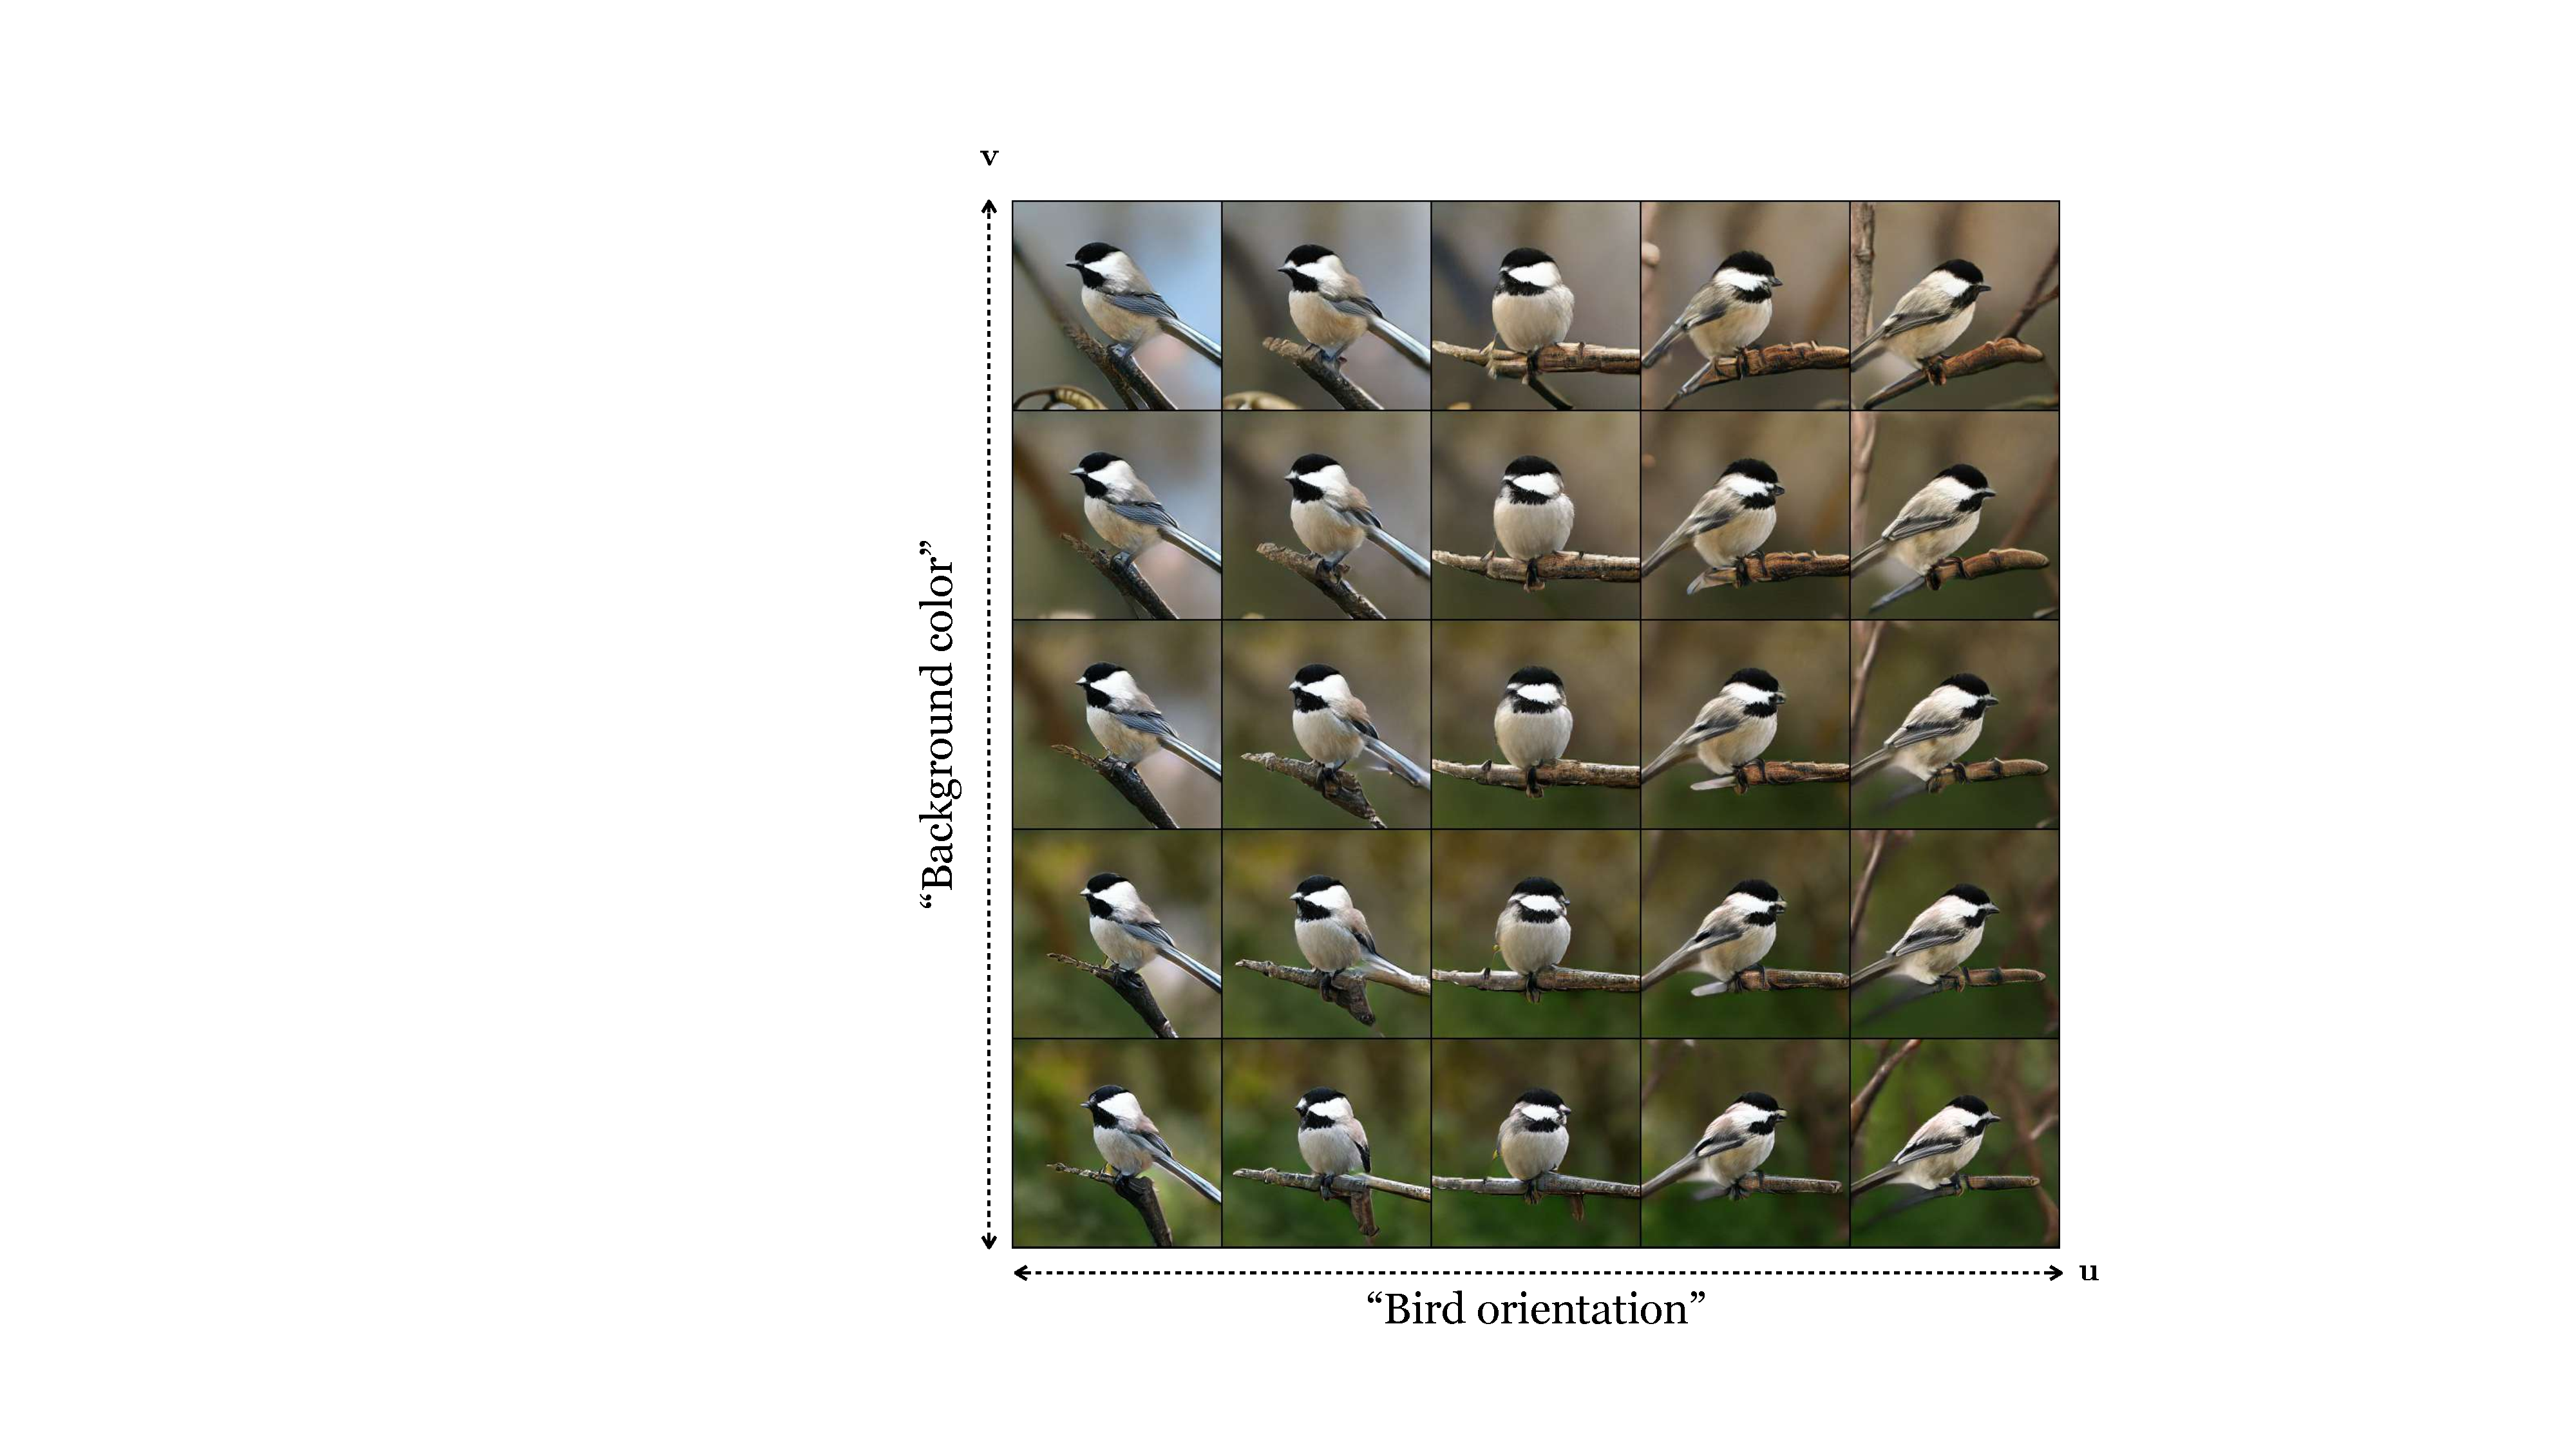
\includegraphics[width=0.6\linewidth]{./figures/generative_modeling_and_representation_learning/biggan_latent_walk.pdf}
    }
    \caption{Walking in in two orthogonal directions in BigGAN~\cite{brock2018large} latent space.}
    \label{fig:generative_modeling_and_representation_learning:biggan_latent_walk}
\end{figure}

Just like with the VAE trained on cartoon rivers, the GAN has also discovered disentangled latent variables; in this case they seem to control background color and the bird's orientation.

This makes sense: structurally, the GAN generator is very similar to the VAE decoder. In both cases, they map a low-dimensional random variable $\mathbf{z}$ to data, and typically $p_{\mathbf{z}} = \mathcal{N}(0,1)$. That means that the dimensions of $\mathbf{z}$ are a priori independent (disentangled). In both models the goal is roughly the same: create synthetic data that has all the properties of real data. It should therefore come as no surprise that both models learn latent representations with similar properties. Indeed, these are just two examples of a large class of models that map low-dimensional latents from a simple (high entropy) distribution to high-dimensional data from a more structured (low entropy) distribution, and we might expect all models in this family to lead to similarly useful representations of the data.

% \subsection{Deep energy-based models}
% One way to think about the discriminator in GANs is as an {\bf energy function} that we want to minimize. While in GANs this energy function changes to penalize whatever current errors the generator is making, would it be possible to learn a ``universal" discriminator that will properly score any type of real or fake imagery and doesn't have to be updated when $G$ changes? This is the idea of {\bf energy-based models}, or {\bf EBMs}.

% With energy-based model, the emphasis is on the energy function, $E$, rather than on the generator -- in fact, there usually is not generator. Instead we can use Markov Chain Monte Carlo (MCMC) to sample from $E$. The energy function is an unnormalized probability distribution, i.e. it is a function $E: \mathcal{X} \rightarrow \mathbb{R}$. We can parameterize $E$ as a neural net -- it's just a net that takes an image as input and produces a real-valued scalar as output.

% MCMC is a method for producing samples from an unnormalized probability distribution, and that's how you sample from an EBM. How do you learn an EBM? First, we definitely want to assign low energy (that is, high probability) to the training datapoints; the first part of the objective of an EBM is to maximize $E(\mathbf{x})$ when $\mathbf{x} \sim p_{data}$. Now, to prevent the energy to go to zero \textit{everywhere} we also need a negative term that will increase energy where there are no datapoints. One option is to just randomly sample ``noise" and increase the energy on this noise. But we can be much more efficient by increasing the energy on ``hard negatives" which are fake images sampled from the current energy function. In particular, it turns out that the gradient of the likelihood function corresponding to an energy-based model has a form that can be evaluated \textit{without normalizing the energies} just by calculating the difference between the energy assigned to real and fake sampled images [XX Turner 2005]:
% \begin{align}
%     \nabla_{\theta}L(\{\mathbf{x}^{(i)}\}_{i=1}^N, \theta) \approx \mathbb{E}_{\mathbf{x} \sim p_{\texttt{data}}}[\nabla_{\theta}E_{\theta(\mathbf{x})}] - \mathbb{E}_{\mathbf{x} \sim p_{E}}[\nabla_{\theta}E_{\theta(\mathbf{x})}]
% \end{align}
% where $p_{E}$ is the normalized energy function $E_{\theta}/Z$; note again that we do not need to compute $Z$ but can still draw samples from $p_{E}$ using MCMC.

% Notice that this objective is very similar to that of a GAN, except:
% \begin{enumerate}
%     \item GANs learn a generator $G$ rather than using MCMC as a sampler that implicitly draws samples from $\frac{E}{Z}$.
%     %\item The GAN discriminator models the \textit{gradient} of an energy function, rather than the energy function itself. Therefore $D$, unlike $E$ cannot be directly used to estimate (unnormalized) likelihoods. 
%     \item The GAN generator is where a lot of the magic of GANs occurs: it is a mapping from low-dimensional latent variables to images. The latent variables turn out to be a remarkably powerful representation of images, with numerous downstream applications. EBMs don't have these latent variables.
% \end{enumerate}



% \section{Normalizing flows}

% Next we will consider generative models with latent variables, $\mathbf{z}$. The models we will cover are implicit: they learn a generator which maps a base distribution over $\mathbf{z}$ to a transformed distribution over $\mathbf{x}$. Typically the base distribution is something simple like $p_{\mathbf{z}} = \mathcal{N}(0,1)$ and the mapping is a deep neural net. The difference between different methods is mainly in the learning objective, which encourages this mapping to fit the data distribution.

% We will start with two implicit max likelihood models, normalizing flows and variational autoencoders. These models share the same objective as autoregressive models -- assign maximum probability density to the training datapoints -- but differ in how they achieve this. For max likelihood models, we need to calculate or approximate the data likelihood function, $L(\{\mathbf{x}^{(i)}\}_{i=1}^N, \theta)$, but how we calculate likelihood can be done in a few ways. In explicit density models, like autoregressive models, we directly learn the likelihood function: $L(\{\mathbf{x}^{(i)}\}_{i=1}^N, \theta) = \prod_i p_{\theta}(\mathbf{x}^{(i)})$. Then we adjust the parameters to maximize this quantity.

% In implicit models, things are a bit harder since we don't have an explicit likelihood function. Instead we learn a generator $G_{\theta}$. If the sampler is bijective, so that $G^{-1}$ exists and can be computed, things are actually still easy. We can use the {\bf change of variables} formula to compute the likelihood of data implied by our sampler:
% \begin{equation*}
%     L(\mathbf{x}, \theta) = p_{\mathbf{z}}(G_{\theta}^{-1}(\mathbf{x}))|\det(\frac{\partial G_{\theta}^{-1}(\mathbf{x})}{\partial \mathbf{x}})| 
% \end{equation*}
% %where $p_{\mathbf{z}}$ is our prior (usually a Normal distribution or uniform distribution).

% Max likelihood learning corresponds to maximizing the log likelihood of the training data, $\{\mathbf{x}^{(i)}\}_{i=1}^N$, so here it looks like:
% \begin{equation}
%     \argmax_{G_{\theta}} \frac{1}{N} \sum_{i=1}^N \log p_{\mathbf{z}}(G_{\theta}^{-1}(\mathbf{x}^{(i)})) + \log |\det(\frac{\partial G_{\theta}^{-1}(\mathbf{x}^{(i)})}{\partial \mathbf{x}^{(i)}})|\label{eqn:generative_models:normalization_flows}
% \end{equation}
% {\bf Normalizing flows} are generative models learned using Equation \ref{eqn:generative_models:normalization_flows}. The name is a reference to the fact that the generator is bijective (a ``flow") and the latent variables have a known (``normalized") density they are drawn from.

% A shortcoming of normalizing flows is that the latent variables have to be of the same dimensionality as the data. Therefore they are not great at representation learning.

%{\bf Diffusion models} are a kind of normalizing flow. They define an invertible process that adds noise to an image in a series of steps. With enough steps, the image because completely random noise. Because each step is invertible, the process can be reversed: first sample random noise, then step by step ``congeal" it into an image. <-- this is wrong, diffusion models are not bijective


\section{Concluding Remarks}

In this chapter we have seen that representation learning and generative modeling are intimately connected; they can be viewed as inverses of each other. This view also reveals an important property of the latent variables in generative models. These variables are like noise in that they are random variables with simple prior distributions, but they are not like our common sense understanding of noise as an unimportant nuisance. In fact, the latent variables can act as a powerful \textit{representation} of the data. You may prefer to think of them as the underlying control knobs that generate the data. A user can spin these knobs randomly to get a random image, or they can tune the knobs navigate the natural image manifold in a systematic way, and arrive at the image they want.